\documentclass[review]{elsarticle}

\usepackage{amsmath}
\usepackage{booktabs}
\usepackage{dirtytalk}
\usepackage{subcaption}
\usepackage{tabularx}
\usepackage{nicefrac}
\usepackage[usenames]{xcolor}
\usepackage{lineno,hyperref}
\modulolinenumbers[5]

\journal{TBA}

%%%%%%%%%%%%%%%%%%%%%%%
%% Elsevier bibliography styles
%%%%%%%%%%%%%%%%%%%%%%%
%% To change the style, put a % in front of the second line of the current style and
%% remove the % from the second line of the style you would like to use.
%%%%%%%%%%%%%%%%%%%%%%%

%% Numbered
%\bibliographystyle{model1-num-names}

%% Numbered without titles
%\bibliographystyle{model1a-num-names}

%% Harvard
%\bibliographystyle{model2-names.bst}\biboptions{authoryear}

%% Vancouver numbered
%\usepackage{numcompress}\bibliographystyle{model3-num-names}

%% Vancouver name/year
%\usepackage{numcompress}\bibliographystyle{model4-names}\biboptions{authoryear}

%% APA style
%\bibliographystyle{model5-names}\biboptions{authoryear}

%% AMA style
%\usepackage{numcompress}\bibliographystyle{model6-num-names}

%% `Elsevier LaTeX' style
\bibliographystyle{elsarticle-num}
%%%%%%%%%%%%%%%%%%%%%%%

\begin{document}

\begin{frontmatter}

\title{Effect of uniform distributions of bonded and debonded fibers on the growth of the fiber/matrix interface crack in thin UD laminates with different fiber contents under transverse loading}
%\tnotetext[mytitlenote]{Fully documented templates are available in the elsarticle package on \href{http://www.ctan.org/tex-archive/macros/latex/contrib/elsarticle}{CTAN}.}

%% Group authors per affiliation:
%\author{Luca Di Stasio\fnref{myfootnote}}
%\address{Radarweg 29, Amsterdam}
%\fntext[myfootnote]{Since 1880.}

%% or include affiliations in footnotes:
\author[nancy,lulea]{Luca Di Stasio}
\author[lulea]{Janis Varna}
\author[nancy]{Zoubir Ayadi}
%\ead[url]{www.elsevier.com}

%\author[mysecondaryaddress]{Global Customer Service\corref{mycorrespondingauthor}}
%\cortext[mycorrespondingauthor]{Corresponding author}
%\ead{support@elsevier.com}

\address[nancy]{Universit\'e de Lorraine, EEIGM, IJL, 6 Rue Bastien Lepage, F-54010 Nancy, France}
\address[lulea]{Lule\aa\ University of Technology, University Campus, SE-97187 Lule\aa, Sweden}

\begin{abstract}
\noindent
\textcolor{purple}{{\em Priority}: 1}\\
\textcolor{purple}{{\em Target journal(s)}: Composites Part B: Engineering, Composites Part A: Applied Science and Manufacturing, Composite Structures, Journal of Composite Materials, Composite Communications}\\

\end{abstract}

%\begin{keyword}
%\texttt{elsarticle.cls}\sep \LaTeX\sep Elsevier \sep template
%\MSC[2010] 00-01\sep  99-00
%\end{keyword}

\end{frontmatter}

\linenumbers

\section{Introduction}

\textcolor{blue}{
\begin{enumerate}
\item We start with a few lines devoted to the spread tow technology and thin plies: what they are, what can be done, what are the possible applications.
\item By quoting the relevant references, we report on the observation that one of the main beneficial mechanisms in thin ply is the retardation of transverse crack propagation. We then enlarge by reporting the microscopical observations by Saito, in which debonds where also observed. We observe that available microscopic observations are just a few and mainly in 2D.
\item Propagation of transverse cracks has been widely investigated both analytically and numerically
\item Initiation at the level of fiber/matrix interface is instead a less researched subject.
\item cohesive elements are a possible choice, but have some drawbacks, which makes a LEFM approach valuable
\item With regard to LEFM studies of laminates under transverse loading, models can be found in the literature about: the single fiber in infinite matrix under different mode of loading, the effect of adjacent fibers on a fiber in infinite matrix under different mode of loading, the single fiber in an equivalent composite in transverse tension, the effect of adjacent fibers on a fiber in an equivalent composite in transverse tension.
\item For initiation of transverse cracking at the fiber/matrix interface in UD laminates under transverse tension, there is thus a gap regarding: the effect of fiber volume fraction; the interaction of debonded and bonded fibers in micro-structured assemblies, i.e. no homogenization. This article addresses these two points.
\item We conclude the introduction with a summary of the article's structure.
\end{enumerate}
}

%%%%%%%%%%%%%%%%%%%%%%%%%%%%%%%%%%%%%%%%%%%%%%%%%%%%%%%%%%%%%%%%%%%
%%%%%%%%%%%%%%%%%%%%%%%%%%%%%%%%%%%%%%%%%%%%%%%%%%%%%%%%%%%%%%%%%%%
\section{RVE models \& FE discretization}

\subsection{Introduction \& Nomenclature}\label{subsec:names}

In this paper, we analyze debond development in unidirectional (UD) composites subjected to in-plane transverse tensile loading.  The interaction between debonds in UD composites is studied developing models of different Repeating Unit Cells (RUC) of laminates where only the central fiber in the cell has a damage in the form of a fiber/matrix interface crack (debond). The composite RUC may be repeating in the transverse direction only (representing an ultra-thin composite) or repeating also in the composite thickness direction, representing an infinite composite in a limiting case. Thus, the conditions at the UD composite's upper and lower boundaries are one of the parameters for the investigation.  The used RUCs allow for the consideration of the composite with debonds as a sequence of damaged and undamaged \say{rows}, each \say{row} with only one fiber in the thickness direction. Since all of these RUCs feature regular microstructures with fibers placed according to a square-packing tiling, they are Representative Volume Elements (RVE) of composites with a certain distribution of debonds. Introducing in-plane coordinates x and y, where x is in the transverse direction of the UD composite under consideration, the strain in the y-direction due to a load in the x-direction is small, due to the very small minor Poisson’s ratio of the UD composite. Additionally, debonds are considered to be significantly longer in the fiber direction than in the arc direction. Therefore, we use 2D models under the assumption of plane strain, defined in the $x-z$ section of the composite.  Thus, the analysis presented applies to long debonds, with a focus on understanding the mechanisms of growth along its arc direction. The composites are subjected to transverse tensile strain, applied as a constant displacement in the $x$-direction along the vertical boundary of the RUC as shown in  Figure~\ref{fig:laminateModelsA} to~\ref{fig:FEmodel}. As the models are differentiated by the number of layers of fibers and by the spacing between debonds along the vertical and horizontal directions, the corresponding RUCs can be distinguished from each other based on the number n of fibers in the horizontal direction and k in the vertical direction. Furthermore, the horizontal surfaces can be either free or vertical displacement coupling can be applied. We thus introduce the common notation$n\times k-free$  and $n\times k-coupling$ to denote a RUC with $n\times k$ fibers and, respectively, a free upper surface or kinematic coupling applied to it. The specific combinations of particular choices of $n$, $k$, and boundary conditions are detailed in Section~\ref{subsec:rve}, together with the corresponding models of damaged composite they are representing.

\subsection{Models of Representative Volume Element (RVE)}\label{subsec:rve}

The first two models feature, as shown in Fig.~\ref{fig:laminateModelsA}, an ultra-thin UD laminate with only one \say{row} of fibers across its thickness, $k=1$. This is quite an extreme model from the microstructural point of view; however, it allows to focus the analysis on the interaction between debonded fibers placed along the x-direction. Furthermore, as the horizontal surfaces are considered free, the interaction is stronger in this case than in any other, making the predictions of this model rather conservative. In retrospective, if only 20 years ago such a model would have been considered too abstracted from the physical reality, the recent advancements in the spread tow technology make this approach appealing also as a limiting case for practical considerations.

\begin{figure}[!h]
\centering
    \begin{subfigure}[b]{\textwidth}
        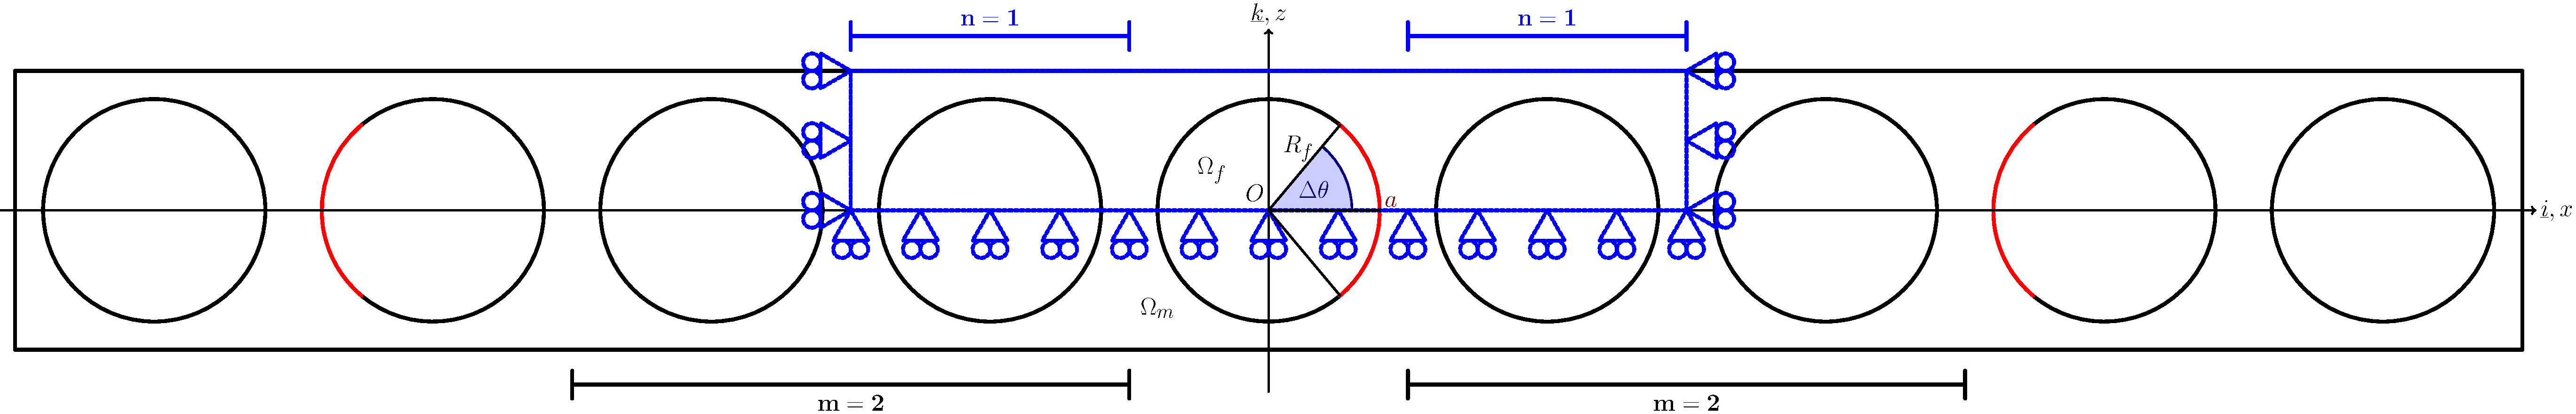
\includegraphics[width=\textwidth]{freeThinPly.pdf}
        \caption{Single \say{row} of fibers with a debond appearing every $m$ fibers.}\label{subfig:freethinply}
    \end{subfigure}

    \begin{subfigure}[b]{\textwidth}
        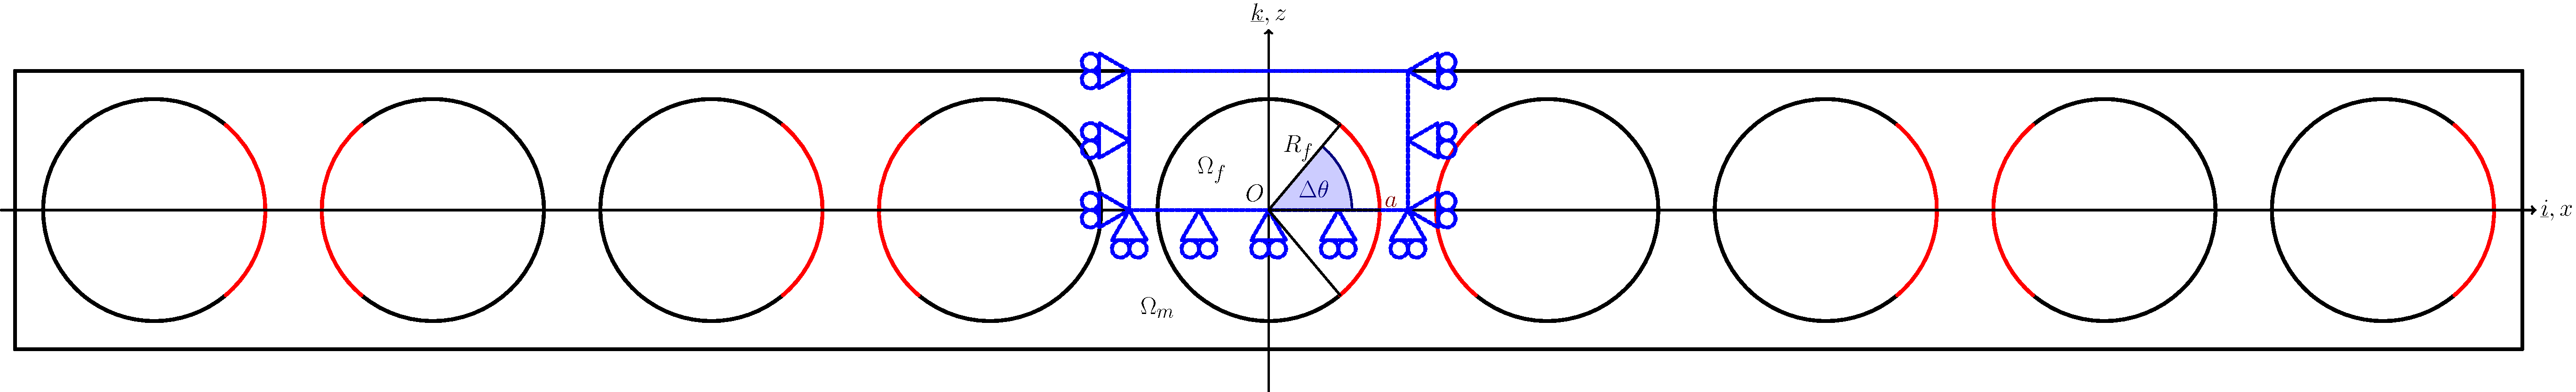
\includegraphics[width=\textwidth]{freeThinPlyAllDebonds.pdf}
        \caption{Single \say{row} of fibers with debonds appearing on each fiber.}\label{subfig:freethinplyalldebonds}
    \end{subfigure}

\caption{Models of ultra-thin UD composites with a single ``row'' of fibers and debonds repeating at different distances. The corresponding repeating element (RUC) is highlighted in blue, while debonds are represented in red.}\label{fig:laminateModelsA}
\end{figure}

In the first sub-model, Fig.~\ref{subfig:freethinply}, every $n^{th}$ fiber in the composite is partially debonded on alternating sides of the fiber. The symmetries of the model allow the use of the upper part of the RUC. It is highlighted by blue lines in Fig.~\ref{fig:laminateModelsA} to~\ref{fig:thickplyalldebonds}. Following the notation introduced in Section~\ref{subsec:names}, we will refer to this model as $n\times 1-free$. In the second sub-model $n=1$, Fig.~\ref{subfig:freethinplyalldebonds}, and a debond appears on each fiber on alternating sides and the corresponding RUC contains only one fiber. We will refer to this model as $1\times 1-free$.

\begin{figure}[!h]
\centering
    \begin{subfigure}[b]{\textwidth}
    \centering
        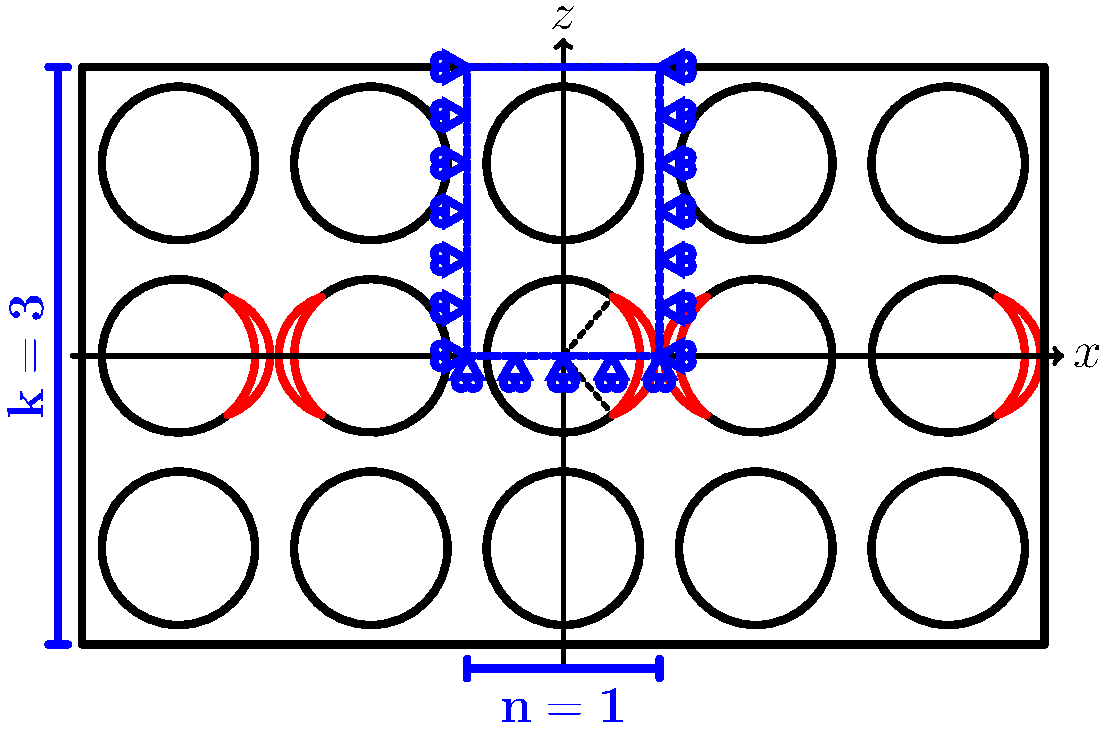
\includegraphics[height=0.3\textheight]{thickPlycentraldebondsline.pdf}
        \caption{Multiple \say{rows} of fibers with debonds appearing on each fiber beloging to the central \say{row}.}\label{subfig:thickplycentraldebonds}
    \end{subfigure}

    \begin{subfigure}[b]{\textwidth}
        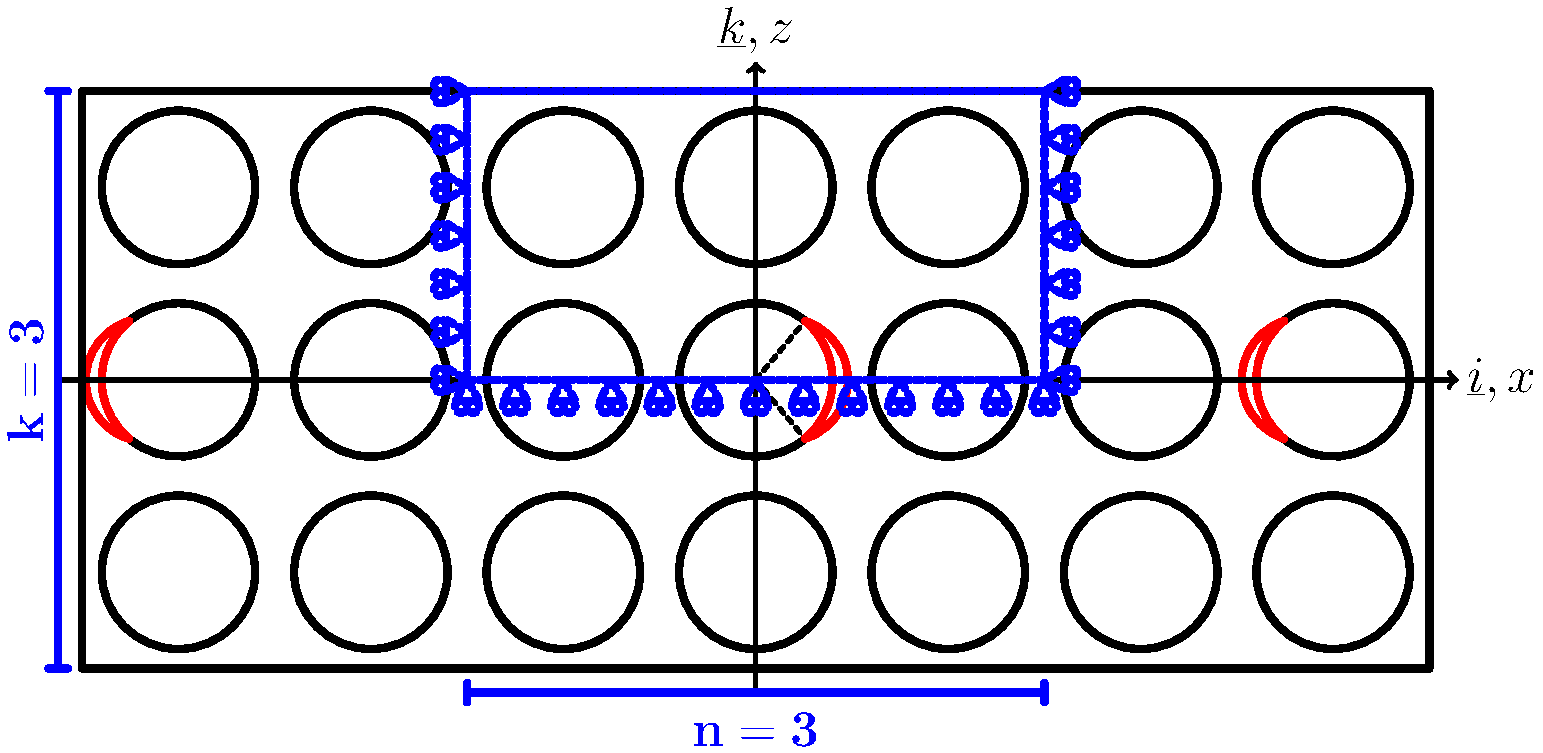
\includegraphics[width=\textwidth]{thickPly.pdf}
        \caption{Mutiple \say{rows} of fibers with a debond appearing every $m$ fibers within the central \say{row}.}\label{subfig:thickply}
    \end{subfigure}

\caption{Models of UD composites with different ``rows'' of fibers and debonds repeating at different distances. The corresponding repeating element (RUC) is highlighted in blue, while debonds are represented in red.}\label{fig:laminateModelsB}
\end{figure}

The second set of models in Fig.~\ref{fig:laminateModelsB} and Fig.~\ref{fig:thickplyalldebonds} considers laminates with multiple \say{rows} of fibers across the thickness: a finite number of rows in the first two sub-models in Fig.~\ref{fig:laminateModelsB}; an infinite number in the model of Fig.~\ref{fig:thickplyalldebonds}. In Fig. ~\ref{subfig:thickplycentraldebonds}, the RUC contains $n=1$ fiber in the x-direction, $k$ fibers across the thickness and the central fiber is debonded. This model will be referred to in the following as $1\times k-free$. Thinking in terms of \say{rows}, in this model we have a central \say{row} where each fiber is debonded. This \say{rows} is surrounded from each side by $\nicefrac{\left(k-1\right)}{2}$ \say{rows} with perfectly bonded fibers. In the sub-model in Fig.~\ref{subfig:thickply}, each $n^{th}$ fiber in the central \say{row} is debonded and this \say{row} is surrounded by $\nicefrac{\left(k-1\right)}{2}$ \say{rows} of undamaged fibers from each side. We will refer to this model as $n\times k-free$ (because the horizontal boundary of the RUC is free of any constraint).

\begin{figure}[!h]
\centering
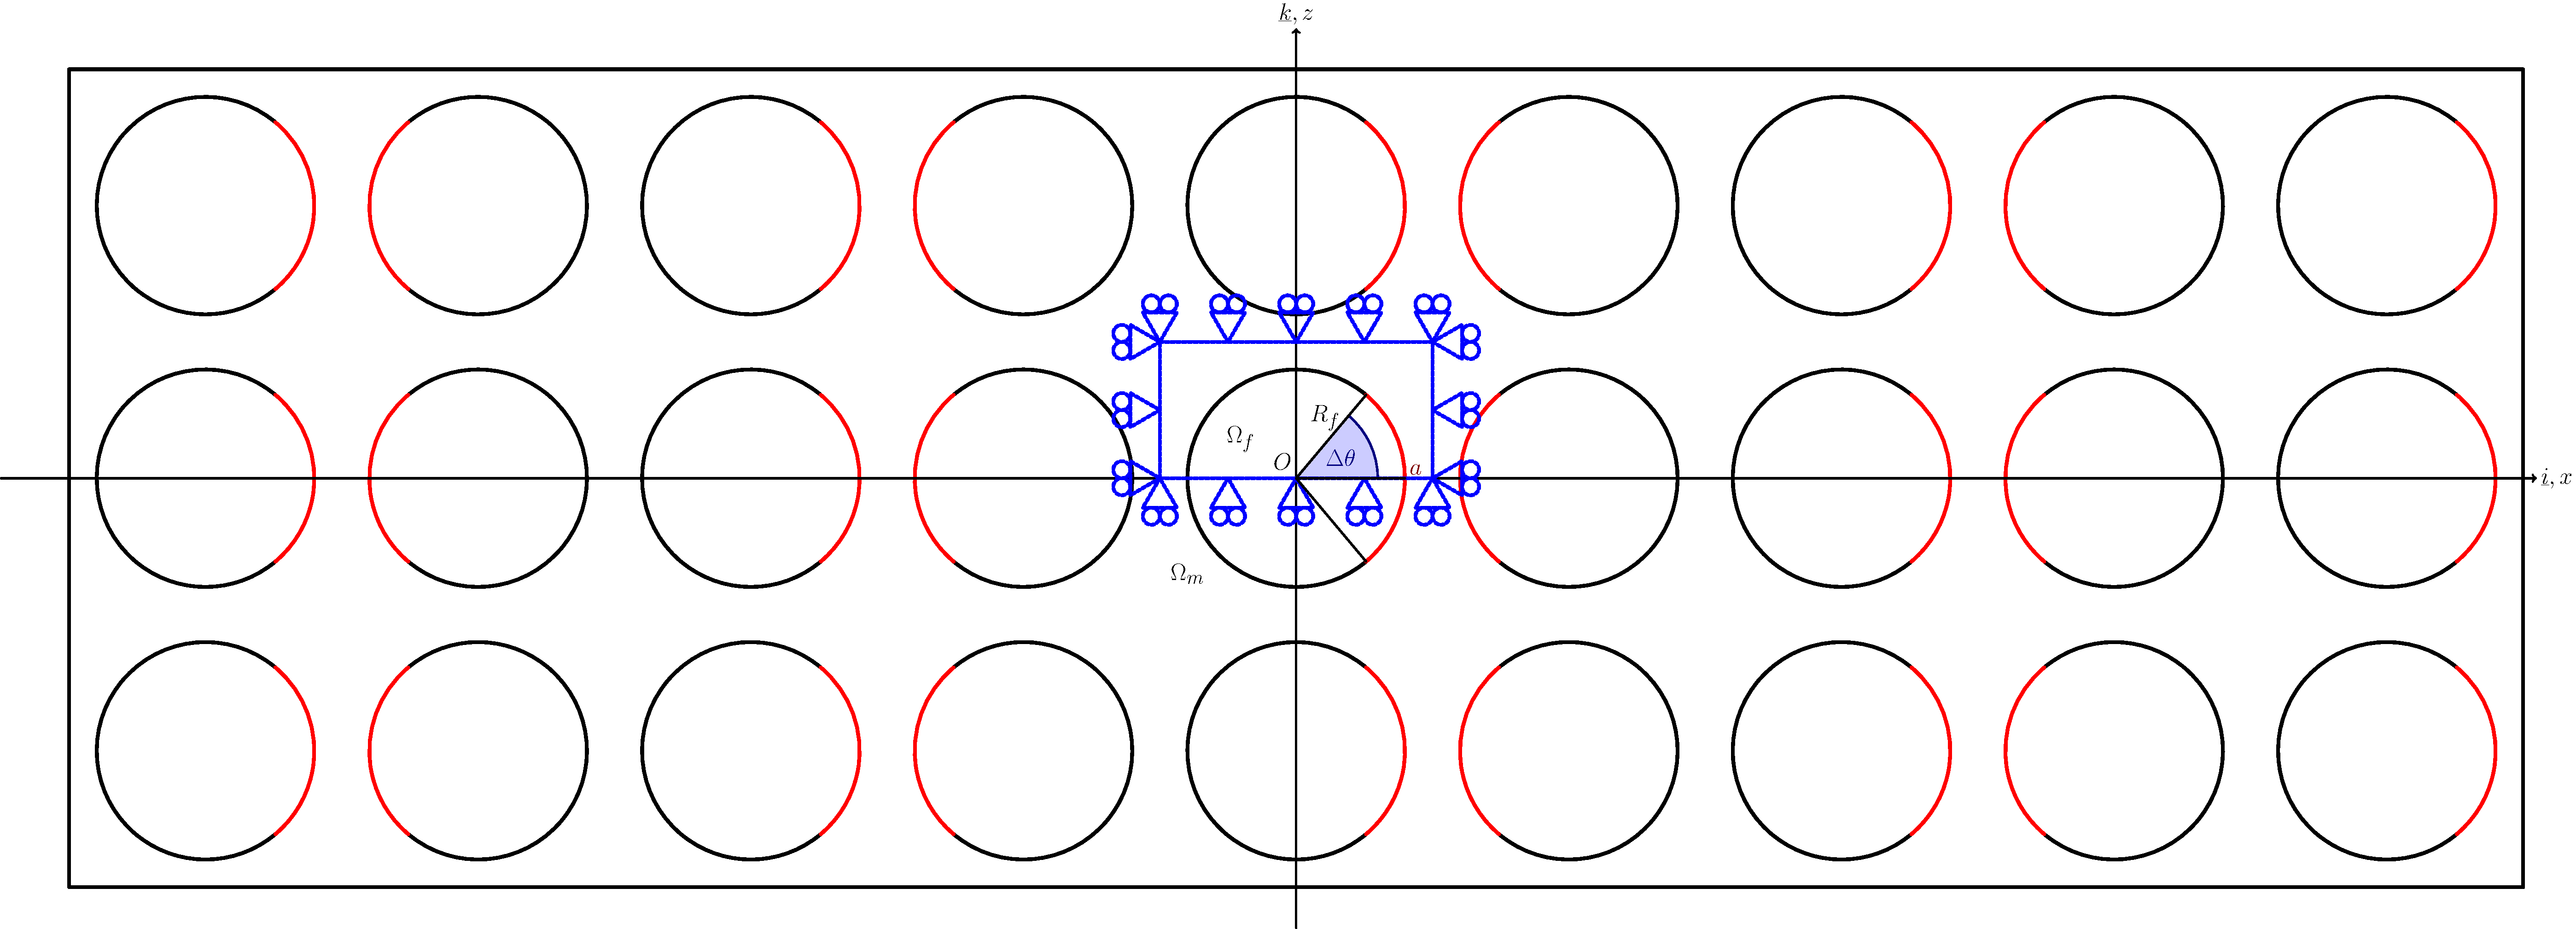
\includegraphics[width=\textwidth]{thickPlyAllDebonds.pdf}
\caption{Model of UD composites with an infinite number of  ``rows'' of fibers and debonds appearing on each fiber. The corresponding repeating element (RUC) is highlighted in blue, while debonds are represented in red.}\label{fig:thickplyalldebonds}
\end{figure}

Finally, the model in Fig.~\ref{fig:thickplyalldebonds} considers an UD composite with an infinite number of \say{rows}; all of them with partially debonded fibers. As all fibers have debonds, the corresponding RUC is made of a single partially debonded fiber with kinematic coupling conditions applied to the upper boundary to assure periodicity. This model is referred to as $1\times 1-coupling$.

%\begin{table}[!h]
% \centering
% \caption{Summary of the models and their characteristics.}
% \begin{tabularx}{\textwidth}{p{0.05\textwidth}ccccc}
%\multicolumn{2}{c}{\textbf{Name}} & \multicolumn{4}{c}{\textbf{Boundary conditions}}\\
%                                                         &  & Up & Down & Right & Left \\
%\toprule
%\midrule
%\multicolumn{2}{c}{$\mathbf{D\left(m+1\right)H0V1L}$} &x-symmetry&free&coupling,&coupling,\\
%                                                         &  &  &  & $\bar{\varepsilon}_{x}=1\%$ & $\bar{\varepsilon}_{x}=1\%$ \\
%&\multicolumn{5}{X}{\small A debond every $\left(m+1\right)^{th}$ fiber in the horizontal direction, in a UD composites with 1 layer of fibers, Fig.~\ref{subfig:freethinply}.}\\
%\midrule
%\multicolumn{2}{c}{$\mathbf{D1H0V1L}$} &x-symmetry&free&coupling,&coupling,\\
%                                                         &  &  &  & $\bar{\varepsilon}_{x}=1\%$ & $\bar{\varepsilon}_{x}=1\%$ \\
%&\multicolumn{5}{X}{\small A debond every $1^{st}$ fiber in the horizontal direction, in a UD composites with 1 layer of fibers, Fig.~\ref{subfig:freethinplyalldebonds}.}\\
%\midrule
%\multicolumn{2}{c}{$\mathbf{D1H0V\left(2p+1\right)L}$} &x-symmetry&free&coupling,&coupling,\\
%                                                         &  &  &  & $\bar{\varepsilon}_{x}=1\%$ & $\bar{\varepsilon}_{x}=1\%$ \\
%&\multicolumn{5}{X}{\small A debond every $1^{st}$ fiber in the horizontal direction, in a UD composites with $\left(2p+1\right)$ layer of fibers, Fig.~\ref{subfig:thickplycentraldebonds}.}\\
%\midrule
%\multicolumn{2}{c}{$\mathbf{D\left(m+1\right)H0V\left(2p+1\right)L}$} &x-symmetry&free&coupling,&coupling,\\
%                                                         &  &  &  & $\bar{\varepsilon}_{x}=1\%$ & $\bar{\varepsilon}_{x}=1\%$ \\
%&\multicolumn{5}{X}{\small A debond every $\left(m+1\right)^{th}$ fiber in the horizontal direction, in a UD composites with $\left(2p+1\right)$ layers of fibers, Fig.~\ref{subfig:thickply}.}\\
%\midrule
%\multicolumn{2}{c}{$\mathbf{D1H1V\infty L}$} &x-symmetry&coupling&coupling,&coupling,\\
%                                                         &  &  &  & $\bar{\varepsilon}_{x}=1\%$ & $\bar{\varepsilon}_{x}=1\%$ \\
%&\multicolumn{5}{X}{\small A debond every $1^{st}$ fiber in the horizontal direction and every $1^{st}$ fiber in the vertical direction, in a UD composites with an infinite number of  layers of fibers, Fig.~\ref{fig:thickplyalldebonds}.}\\
%\bottomrule
%\end{tabularx}
%\label{tab:modelcharacteristics}
%\end{table}
%
%A summary of models' names and characteristics is reported in Table~\ref{tab:modelcharacteristics}

\subsection{Finite Element (FE) discretization}

Each RUC is discretized using the Finite Element Method (FEM) within the Abaqus environment, a commercial FEM package~\cite{abq12}. The length $l$ and height $h$ of the model are determined by number of fibers $n$ in the horizontal direction and $k$ across the thickness (see~\ref{subsec:rve}) according to Eq.~\ref{eq:lengthheight}:

\begin{equation}\label{eq:lengthheight}
l=2nL\qquad h=2kL;
\end{equation}

where the reference length $L$, see Fig.~\ref{subfig:modelschem}, is defined as a function of the fiber volume fraction $V_{f}$ and the fibers' radius according to

\begin{equation}\label{eq:LVf}
L=\frac{R_{f}}{2}\sqrt{\frac{\pi}{V_{f}}}.
\end{equation}

The fibers' radius $R_{f}$ is assumed to be the same for each fiber present in the model and equal to $1\ \mu m$. The latter value is not physical and it has been chosen for simplicity. It is worth to note at this point that, in a linear elastic solution as the one presented here, the ERR is proportional to the geometrical dimensions and recalculation of the ERR for fibers of any size thus requires a simple multiplication. Furthermore, notice that the relationships in Eqs.~\ref{eq:lengthheight} and~\ref{eq:LVf} ensure that the local and global $V_{f}$ are everywhere equal.

\begin{figure}[!h]
\centering
    \begin{subfigure}[b]{0.55\textwidth}
        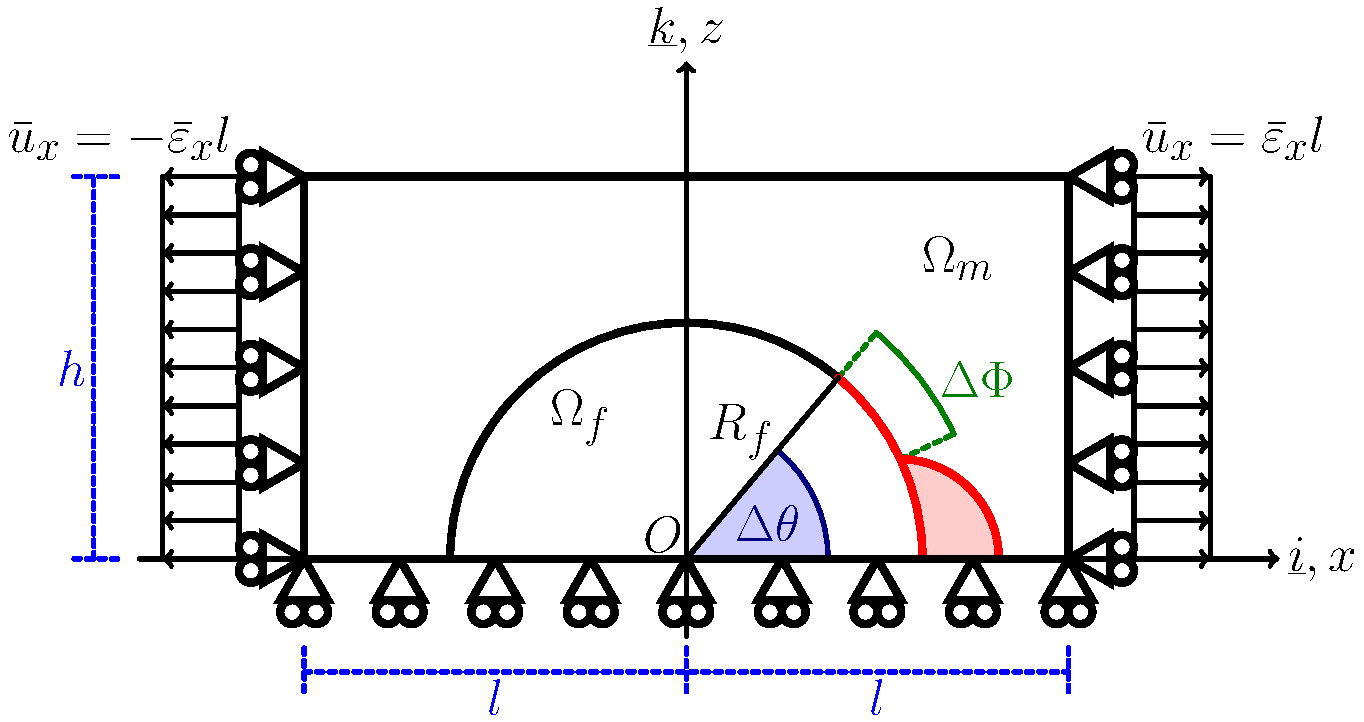
\includegraphics[width=\textwidth]{RUC.pdf}
        \caption{Schematic of the model with its main parameters.}\label{subfig:modelschem}
    \end{subfigure} ~
    \begin{subfigure}[b]{0.4\textwidth}
        \includegraphics[width=\textwidth]{mesh-detail.eps}
        \caption{Mesh near the crack tip. Crack's faces shown in red.}\label{subfig:meshdetail}
    \end{subfigure}

\caption{Details and main parameters of the Finite Element model.}\label{fig:FEmodel}
\end{figure}

The debond is placed symmetrically with respect to the $x$ axis (in red in~\ref{subfig:modelschem}) and has an angular size of $\Delta\theta$ (the full debond's size is thus $2\Delta\theta$). For large debond's sizes ($\geq 60^{\circ}-80^{\circ}$), a region of variable size $\Delta\Phi$ appears at the crack tip in which the crack's faces are in contact and slide on each other. Due to its appearance, frictionless contact is considered between the two crack's faces to allow free sliding and avoid interpenetration. Symmetry with respect to the $x$ axis is applied on the lower boundary and kinematic coupling on the $x$-displacement along the left and right sides. The upper boundary is in general free, except for the model $1\times 1-coupling$ (Fig.~\ref{fig:thickplyalldebonds}) which requires kinematic coupling of vertical displacements also on the upper side. Constant transverse strain $\bar{\varepsilon}$ equal to $1\%$ is applied to the right and left sides by means of an imposed $x$-displacement of, respectively, $\pm\bar{\varepsilon}l$.

\begin{table}[!htbp]
 \centering
 \caption{Summary of the mechanical properties of fiber and matrix.}
 \begin{tabular}{cccc}
\textbf{Material} & \textbf{$E\left[GPa\right]$}\ & \textbf{$G\left[GPa\right]$} & \textbf{$\nu\left[-\right]$} \\
\midrule
Glass fiber    & 70.0  & 29.2   & 0.2  \\
Epoxy    & 3.5    & 1.25   & 0.4
\end{tabular}
\label{tab:phaseprop}
\end{table}

The model is meshed using second order, 2D, plane strain triangular (CPE6) and rectangular (CPE8) elements. A regular mesh of quadrilateral elements with an almost unitary aspect ratio is required at the crack tip, as shown in Fig.~\ref{subfig:meshdetail}. The angular size $\delta$ of an element in the crack tip region is always equal to $0.05^{\circ}$. The Mode I, Mode II and total Energy Release Rates (ERRs) (respectively referred to as $G_{I}$, $G_{II}$ and $G_{TOT}$) represent the main output of the FEM analysis; they are evaluated using the VCCT technique~\cite{Krueger2004} implemented in a custom Python routine and, for the total ERR, the J-integral~\cite{Rice1968} by application of the Abaqus built-in functionality. A glass fiber-epoxy system is considered in every model, and it is assumed that their response lies always in the linear elastic domain. The properties used are listed in Table~\ref{tab:phaseprop}.

\subsection{Validation of the model}

The model is validated in Fig.~\ref{fig:validation} against the results reported in~\cite{Sandino2016}, obtained with the Boundary Element Method (BEM) for a single fiber with a symmetric debond placed in an infinite matrix. This situation is modeled using the \textit{free} RVE with $V_{f}=0.0079\%$, which corresponds to a RUC's length and height of $\sim 100$.

\begin{figure}[!h]
\centering
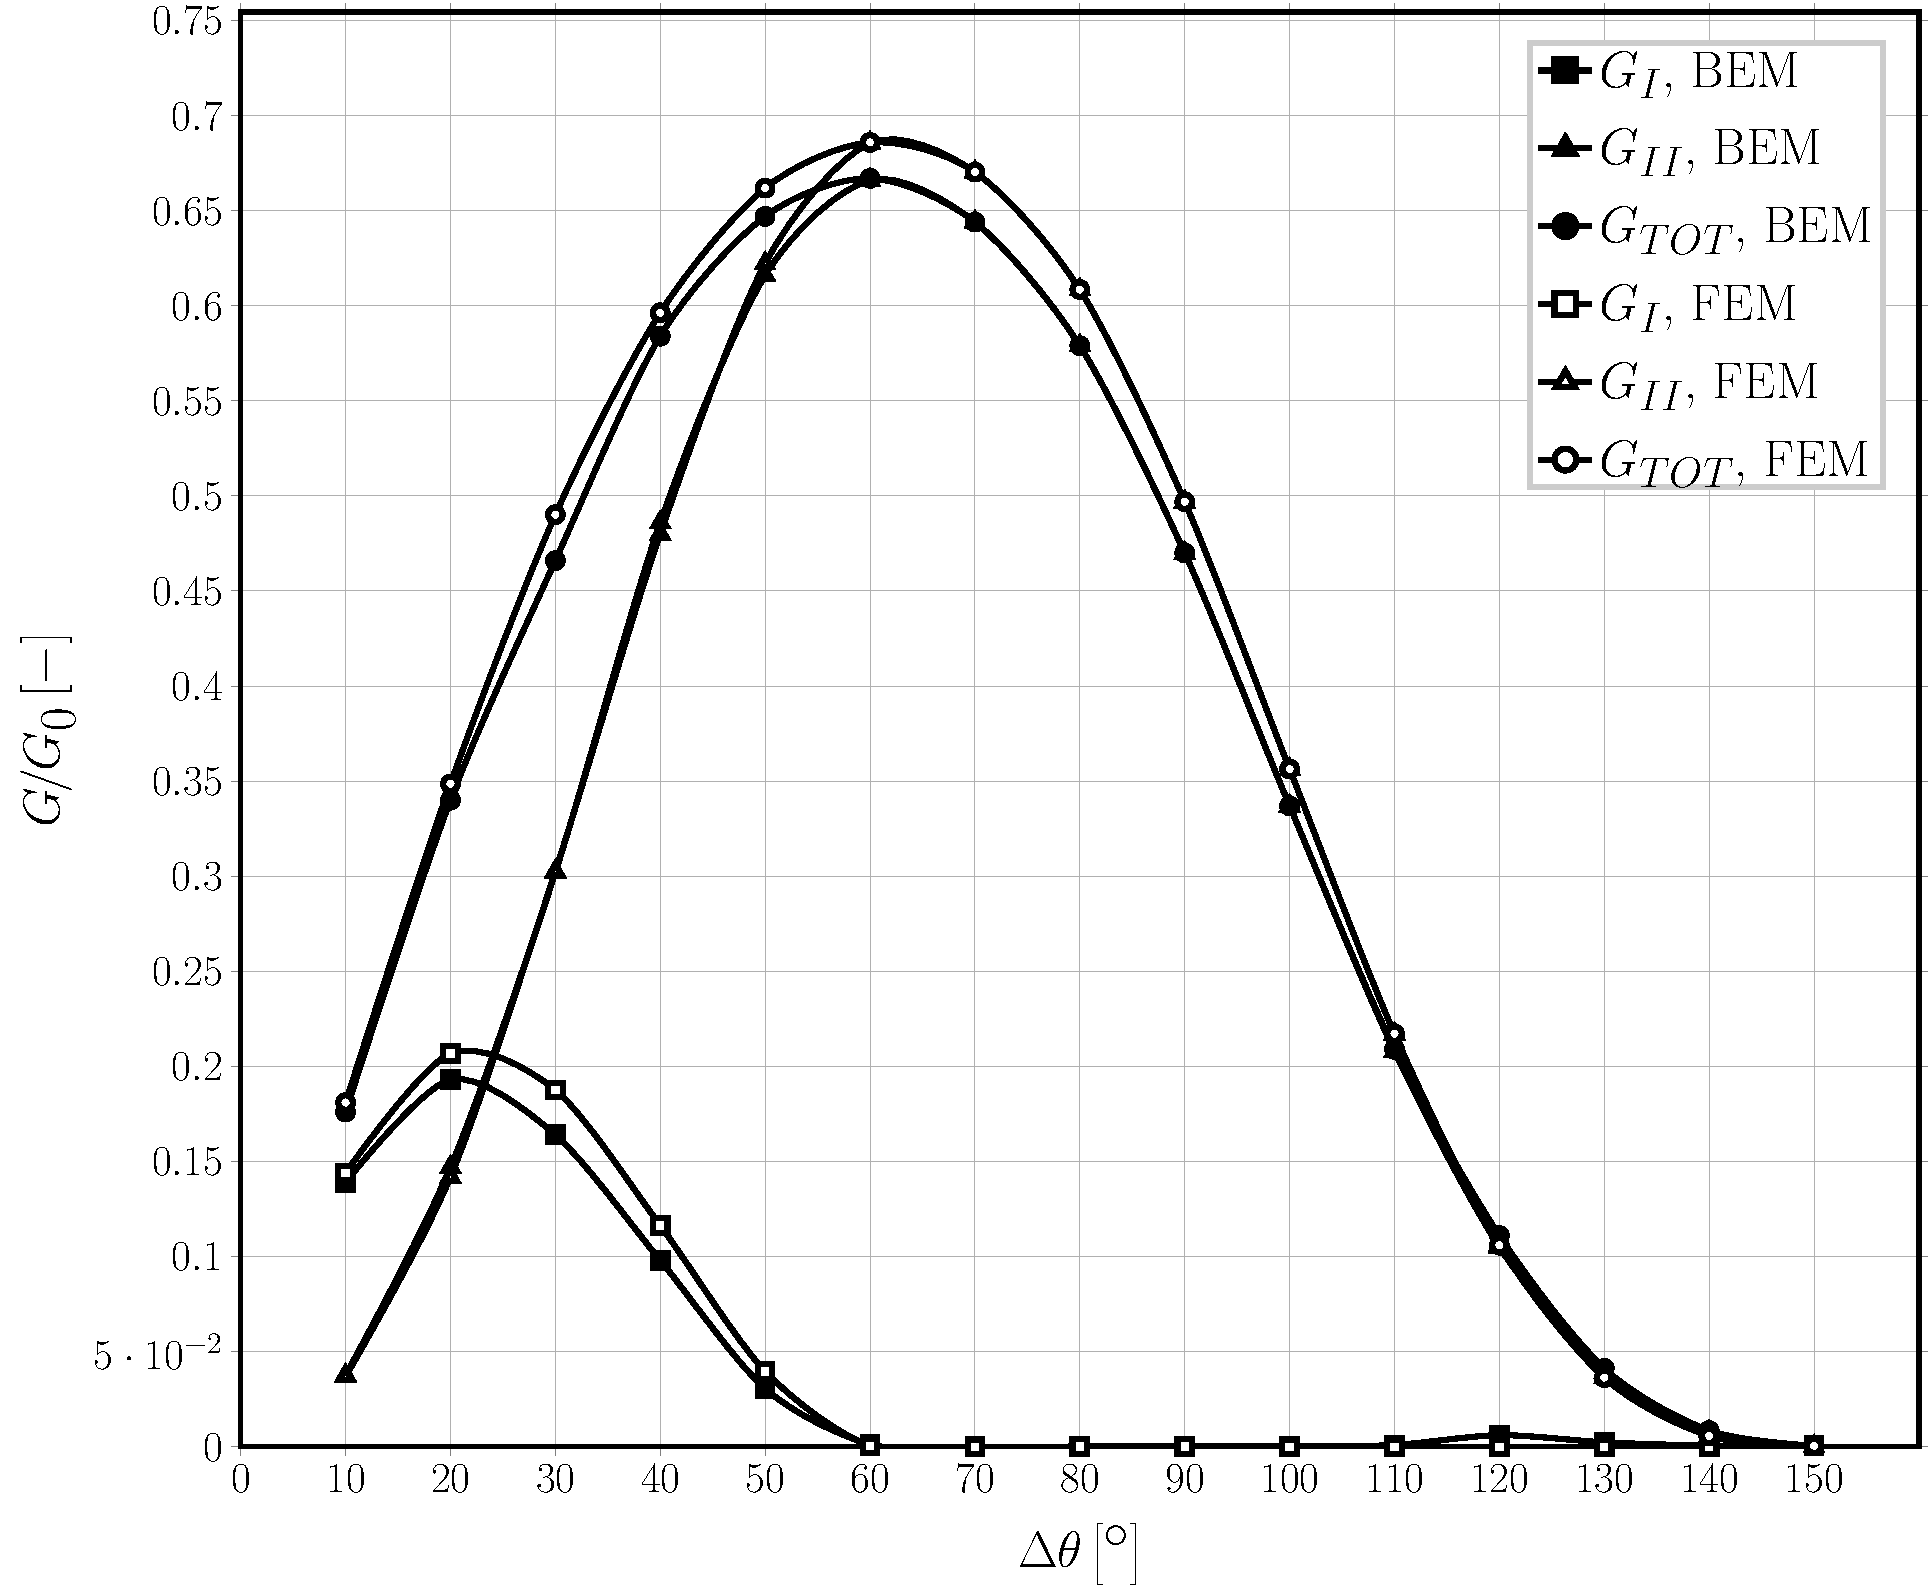
\includegraphics[width=\textwidth]{validation-VCCT.pdf}
\caption{Validation of the single fiber model for the infinite matrix case with respect to the BEM solution in \cite{Sandino2016}.}\label{fig:validation}
\end{figure}

To allow for a comparison, the results are normalized following~\cite{Sandino2016} with respect to a reference Energy Release Rate $G_{0}$ defined as

\begin{equation}
G_{0}=\frac{1+k_{m}}{8\mu_{m}}\sigma_{0}^{2}\pi R_{f}
\end{equation}

where $\mu$ is the shear modulus, $k$ is the Kolosov's constant defined as $3-4\nu$ for plane strain conditions, $R_{f}$ is the fiber radius and the index $m$ refers to the properties of the matrix. $\sigma_{0}$ is the stress at the boundary, computed as the average of the stress extracted at each boundary node along the right side (arithmetic average as nodes are equispaced by design along both the left and right sides). The agreement is good: the difference between the BEM solution, which is considered more accurate, and the FEM solution does not exceed $5\%$. The ERRs' maxima are in the same positions and the size of the contact zone is the same.  Nevertheless, an analysis of phenomena leading to less than $5\%$ differences in ERR would not be reliable and, therefore, it is not recommended.

%%%%%%%%%%%%%%%%%%%%%%%%%%%%%%%%%%%%%%%%%%%%%%%%%%%%%%%%%%%%%%%%%%%
%%%%%%%%%%%%%%%%%%%%%%%%%%%%%%%%%%%%%%%%%%%%%%%%%%%%%%%%%%%%%%%%%%%

\section{Results \& Discussion}

\subsection{Effect of Fiber Volume Fraction}\label{subsec:volfrac}

As shown in Figs.~\ref{fig:volumefractionMI} and~\ref{fig:volumefractionMII}, respectively for Mode I and Mode II, the fiber content has a drastic effect on the Energy Release Rate at the tip of the fibre/matrix interface crack. The effect of four levels of fiber volume fraction are compared, $30\%$, $50\%$, $60\%$ and $65\%$, on two microstructural models: a $11\times 11-free$ (every $11^{th}$ fiber in the central fiber \say{row} is partially debonded and, on the top of this \say{row}, we have 5 undamaged fiber \say{rows}), Figs.~\ref{subfig:volfracsmallerMI} and~\ref{subfig:volfracsmallerMII}, and a $21\times 21-free$ (every $21^{th}$ fiber in the central fiber \say{row} is partially debonded and, on the top of this \say{row}, we have 10 undamaged fiber \say{rows}), Figs.~\ref{subfig:volfracbiggerMI} and~\ref{subfig:volfracbiggerMII}.

\begin{figure}[!h]
\centering
    \begin{subfigure}[b]{0.475\textwidth}
        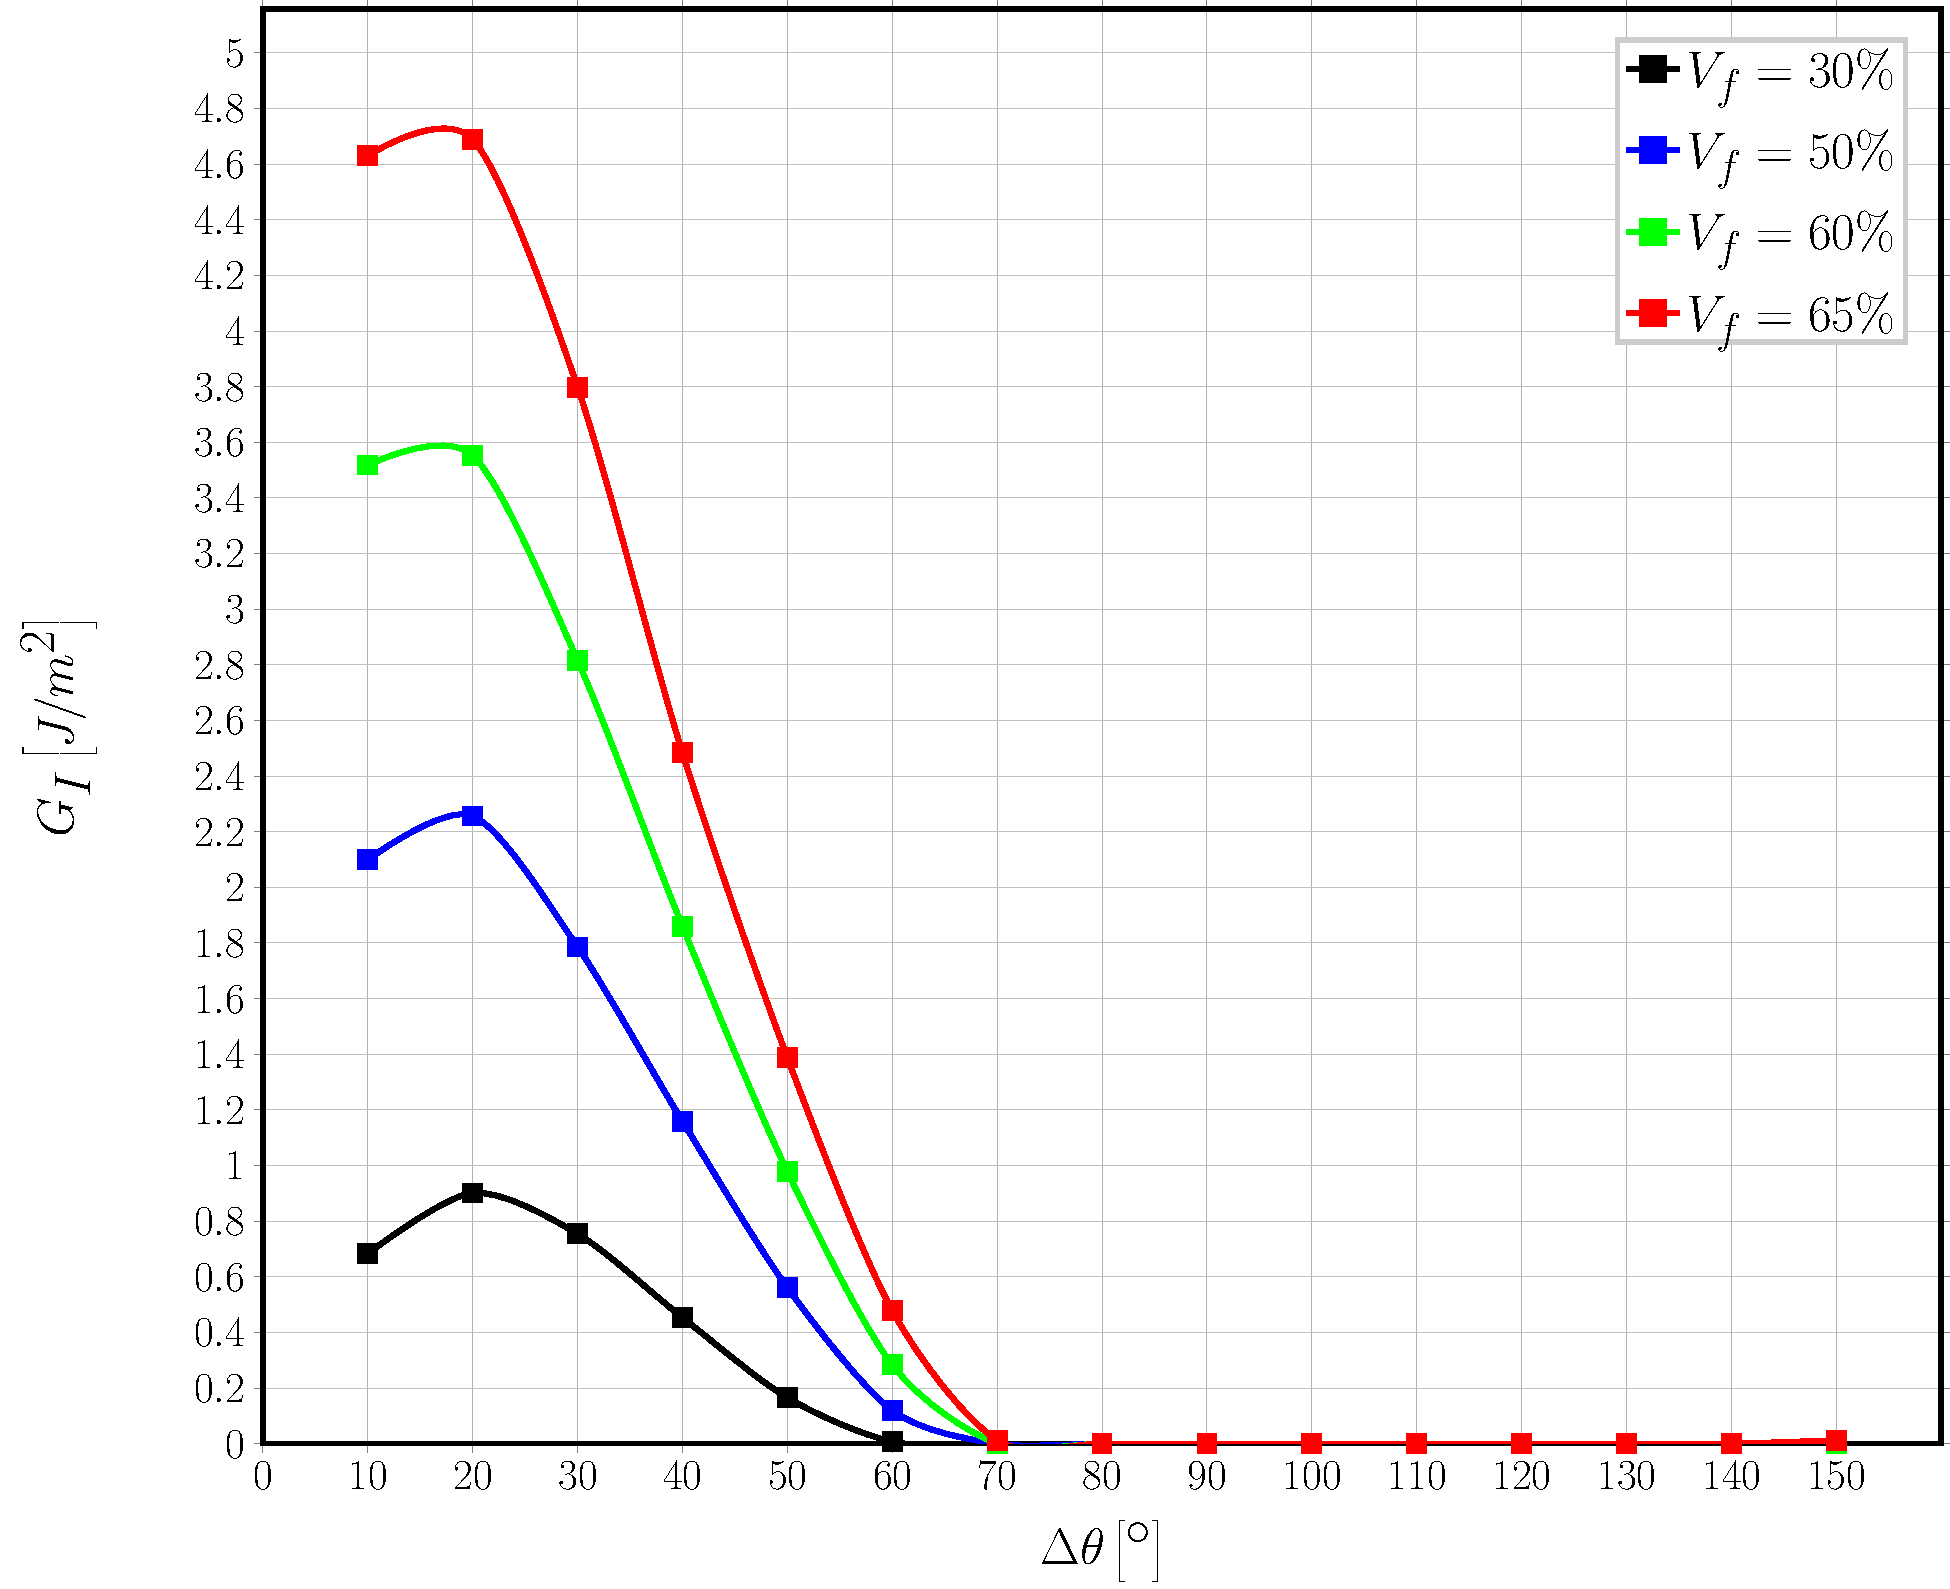
\includegraphics[width=\textwidth]{vf-smallermodel-GI.pdf}
        \caption{5 fibers each side, 5 above.}\label{subfig:volfracsmallerMI}
    \end{subfigure} ~
    \begin{subfigure}[b]{0.475\textwidth}
        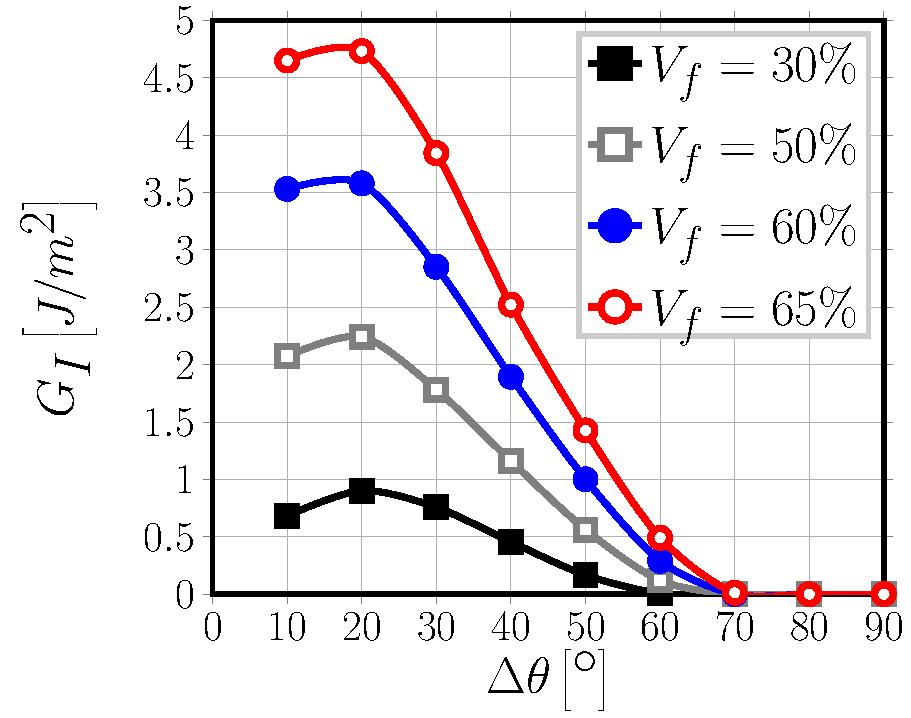
\includegraphics[width=\textwidth]{vf-biggermodel-GI.pdf}
        \caption{10 fibers each side, 10 above.}\label{subfig:volfracbiggerMI}
    \end{subfigure}

\caption{A view of the effect of fiber volume fraction on Mode I ERR in two exemplificative models.}\label{fig:volumefractionMI}
\end{figure}

Comparison of Fig.~\ref{subfig:volfracsmallerMI} with~\ref{subfig:volfracbiggerMI}, and of Fig.~\ref{subfig:volfracsmallerMII} with~\ref{subfig:volfracbiggerMII}, indicates that there exists a specific effect of the fiber content, independent of the microstructure. For Mode I, Fig.~\ref{fig:volumefractionMI}, the maximum value of the ERR is increased by $\sim 5.2$ times when $V_{f}$ changes from $30\%$ to $65\%$ in both models. The debond's size for which the peak value occurs remains unchanged at $20^{\circ}$, but for $60\%$ and $65\%$ the value at $10^{\circ}$ and at $20^{\circ}$ are almost identical, approximately creating a plateau and thus making the growth of small debonds ($\leq 20^{\circ}$) in Mode I unstable. Furthermore, increasing the fiber volume fraction delays the onset of the contact zone, which corresponds in~\ref{fig:volumefractionMI} to the first value of $\Delta\theta$ for which $G_{I}$ is equal to zero. For $V_{f}=30\%$, the contact zone first appears for a debond of $60^{\circ}$, similarly to what happens in the single fiber in infinite matrix model (Fig.~\ref{fig:validation}). For higher fiber contents, the contact zone's onset is delayed to a debond's size equal to $70^{\circ}$.

\begin{figure}[!h]
\centering
    \begin{subfigure}[b]{0.475\textwidth}
        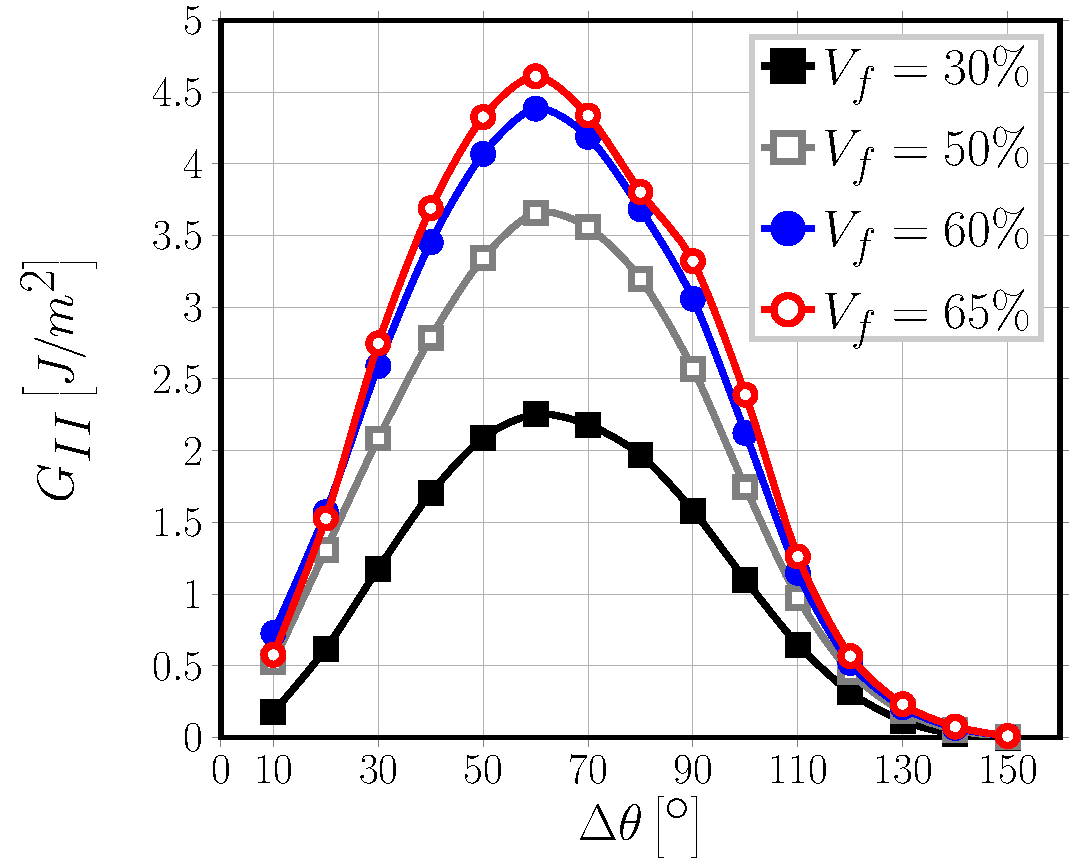
\includegraphics[width=\textwidth]{vf-smallermodel-GII.pdf}
        \caption{5 fibers each side, 5 above.}\label{subfig:volfracsmallerMII}
    \end{subfigure} ~
    \begin{subfigure}[b]{0.475\textwidth}
        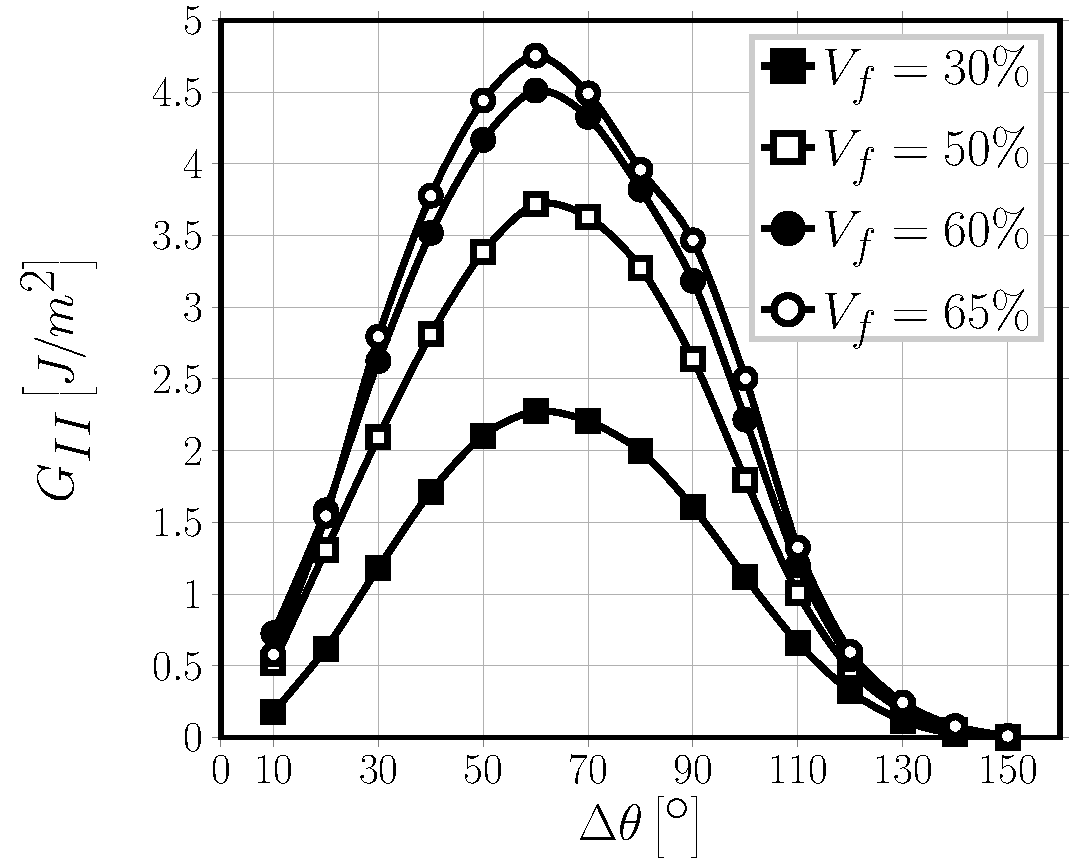
\includegraphics[width=\textwidth]{vf-biggermodel-GII.pdf}
        \caption{10 fibers each side, 10 above.}\label{subfig:volfracbiggerMII}
    \end{subfigure}

\caption{A view of the effect of fiber volume fraction on Mode II ERR in two exemplificative models.}\label{fig:volumefractionMII}
\end{figure}

For Mode II, Fig.~\ref{fig:volumefractionMI}, the maximum value of the ERR is increased by $\sim 2.1$ times when $V_{f}$ changes from $30\%$ to $65\%$ in both models. The effect is thus similar to Mode I, but with a significantly lower magnitude. As for Mode I, the debond's size for which the peak value occurs remains unchanged, at $60^{\circ}$ for Mode II. The shape of the curve remains instead unchanged, thus no effect on the stability of Mode II with respect to debond's size can be observed. It is worthwhile to notice, however, that the ratio of Mode II to Mode I peak values is $\frac{max\left(G_{II}\right)}{max\left(G_{I}\right)}\sim\frac{2.2}{0.9}\sim 2.4$ for $V_{f}=30\%$, while it is $\sim\frac{4.7}{4.7}\sim 1$ for $V_{f}=65\%$ in both models. Given that the peaks occur at different debond's sizes, for which the value of the other ERR is very small or even close to zero, this means that the increase in fiber content creates a long range of very close values of total ERR, and thus has a global destabilizing effect on the debond's growth.\\
The general incresing trends observed in Figs.~\ref{fig:volumefractionMI} and~\ref{fig:volumefractionMII} are related to the fact that, given that the global and local $V_{f}$ are everywhere identical in the models presented, an increase in fiber content corresponds to a decrease in the average distance between fibers. Thus, the relaxation of the stress and strain fields in the matrix domain occurs over smaller lengths causing higher values at the crack tip. The difference in relative magnification between Mode I and Mode II and the delay in the contact zone's onset are instead due to the interplay between two different mechanisms, both caused by the ordered microstructural arrangement of the model. In the models considered, a fully bonded fiber is always placed along the horizontal direction, aligned with the partially debonded fiber and exactly in front of the debond. By increasing $V_{f}$, the former moves closer to the latter and this causes a magnification of the x-strain at the crack tip. For small debonds ($\leq 20^{\circ}-30^{\circ}$), the crack tip is approximately normal to the x-direction and thus an increase in $\varepsilon_{x}$ causes an increase in $G_{I}$. On the other hand, for large debonds ($\geq 70^{\circ}-80^{\circ}$) the crack growth is almost aligned with the x-axis, thus a magnification in the x-strain translates into an increase of Mode II ERR. However, this increasing effect on $G_{II}$ is counteracted by the presence of a fully bonded fiber along the vertical direction, aligned with the partially debonded one. As fibers are more rigid than the sourrounding matrix, the presence of the former will restrain horizontal displacements, thus hampering strong increases in $G_{II}$ for large debonds. Furthermore, due to the mismatch in the Poisson's ratios, the fully bonded fiber placed above generates an upward-directed component of the vertical displacement field in the matrix, which tends to open the debond and causes the delay in the contact zone's onset. The interplay between these mechanisms is governed by the average inter-fiber distance and, in turn, by the fiber volume fraction.

\subsection{Interaction between debonds in UD laminates with a single layer of fibers}\label{subsec:singlefiberud}

The interaction of debonds appearing at regular intervals in UD composites with a single layer of fibers is studied for Mode I (Fig.~\ref{fig:sidefibersMI}) and Mode II (Fig.~\ref{fig:sidefibersMII}) and fiber content equal to $30\%$ (Figs.~\ref{subfig:sidefiber30MI} and~\ref{subfig:sidefiber30MII}) and $60\%$ (Figs.~\ref{subfig:sidefiber60MI} and~\ref{subfig:sidefiber60MII}). The models treated are $3\times 1-free$, $5\times 1-free$, $7\times 1-free$, $11\times 1-free$, $21\times 1-free$, $101\times 1-free$ and $201\times 1-free$, corresponding respectively to a debond every $3^{rd}$, $5^{th}$, $7^{th}$, $11^{th}$, $21^{st}$, $101^{st}$ and $201^{st}$ fiber (Fig.~\ref{subfig:freethinply}). Given that the upper surface of the UD is left free, the interaction is stronger than in any other case and the results of this section are thus the most conservative in terms of debond's growth. From both~\ref{fig:sidefibersMI} and~\ref{fig:sidefibersMII}, it can be seen that the presence of a debond decreases the strain magnification effect discussed in Sec.~\ref{subsec:volfrac} and thus reduces the value of the ERR.

\begin{figure}[!h]
\centering
    \begin{subfigure}[b]{0.475\textwidth}
        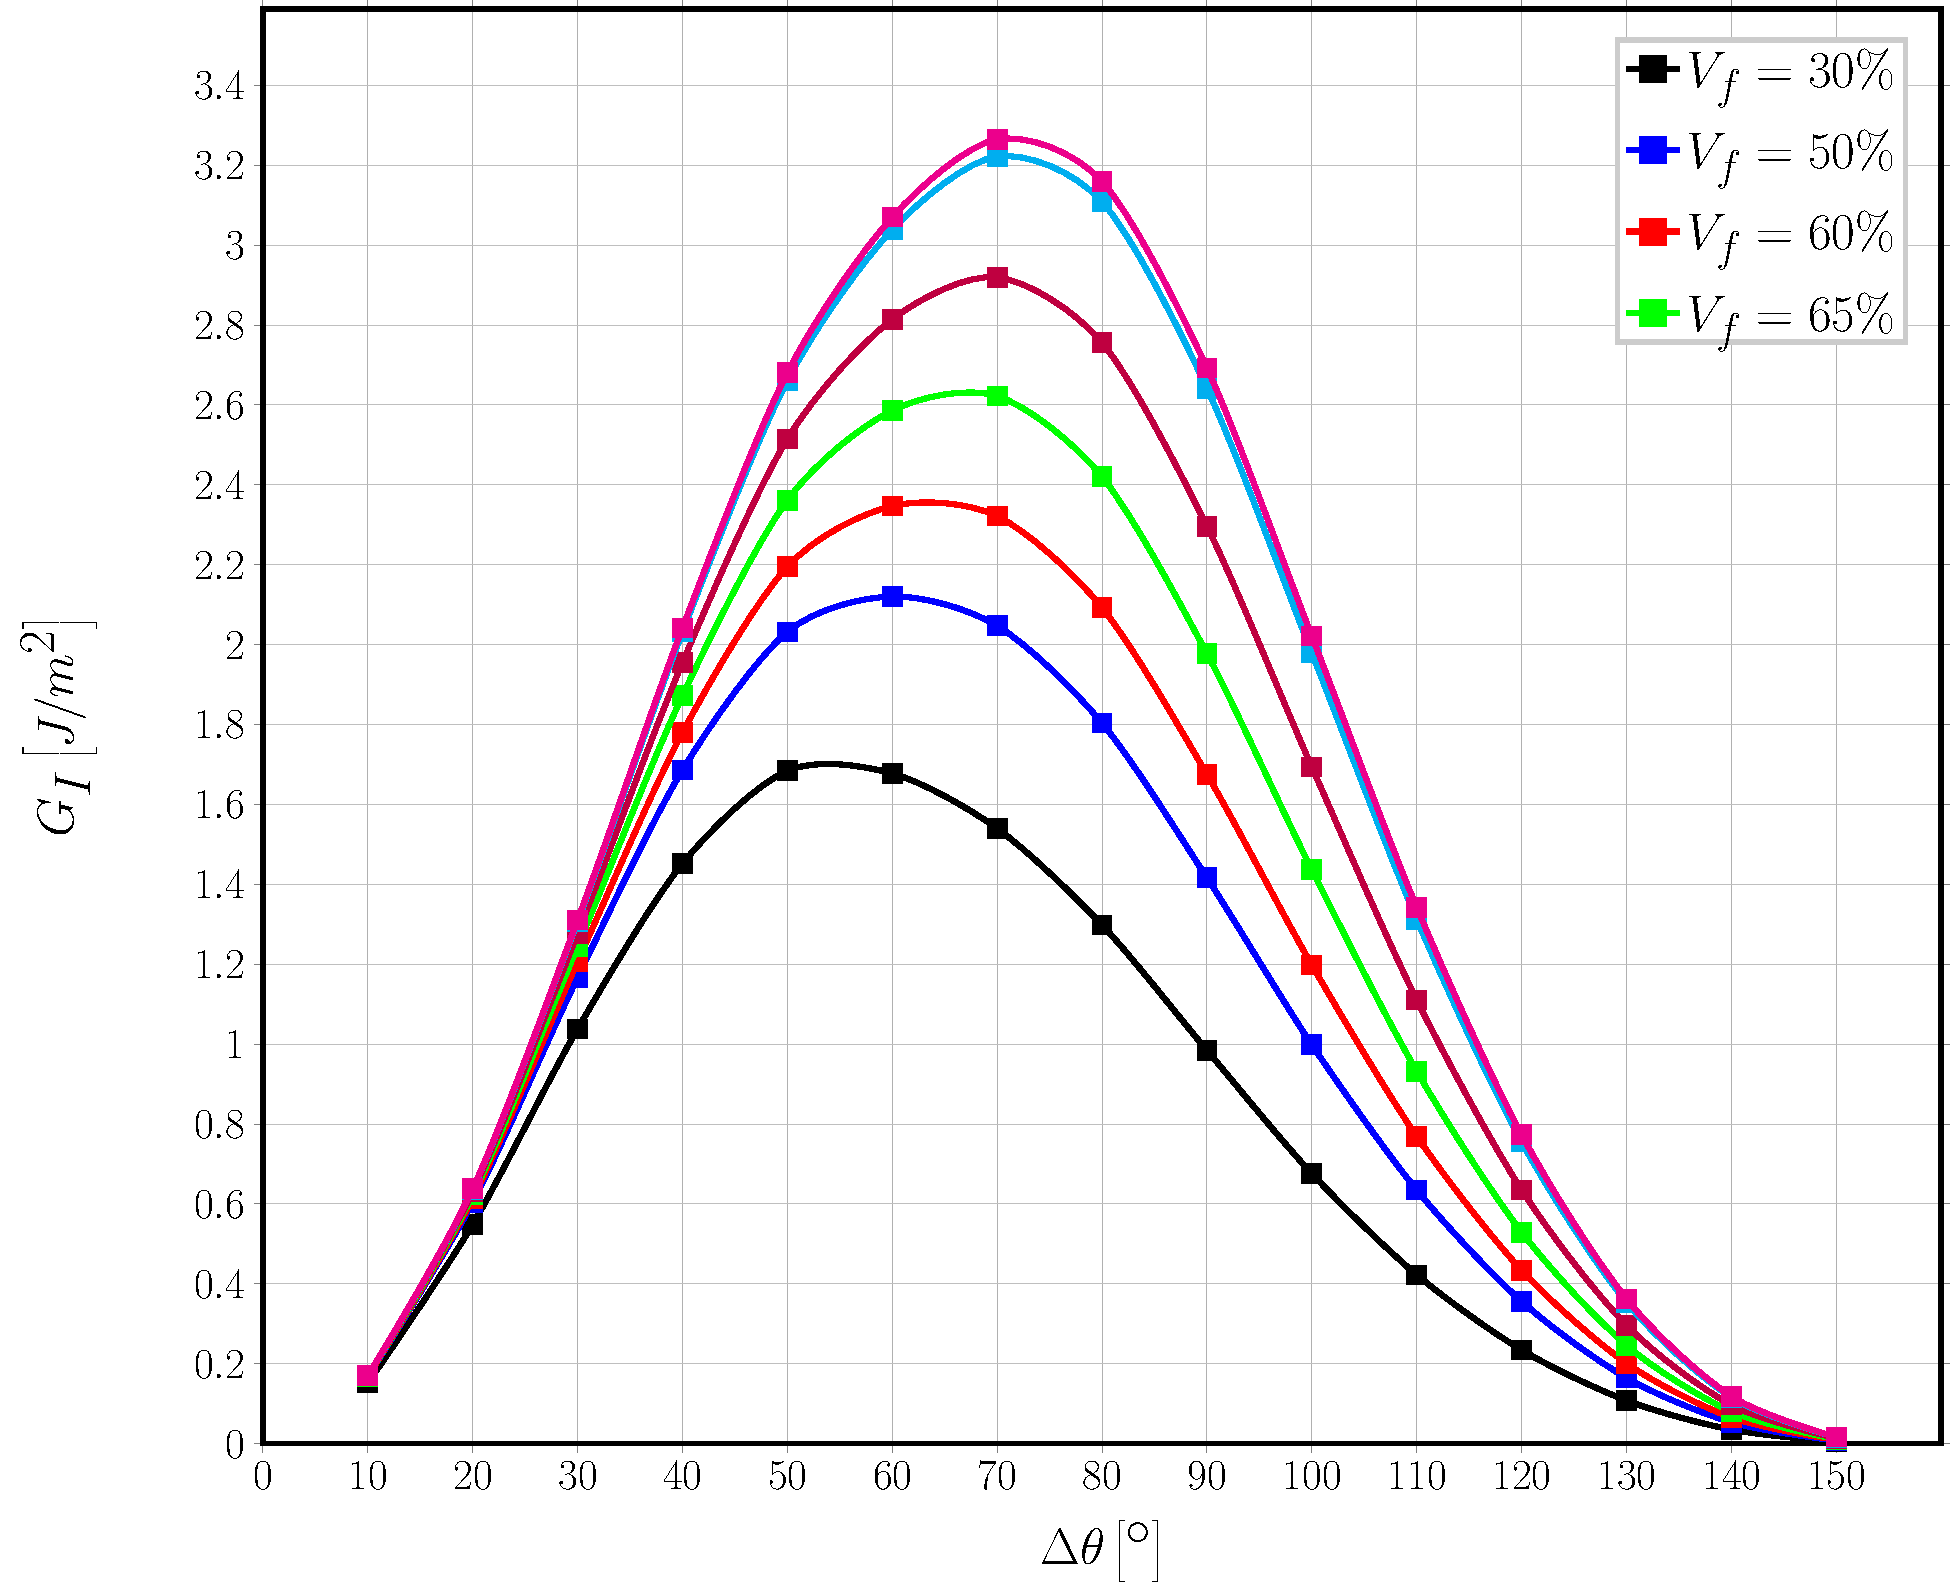
\includegraphics[width=\textwidth]{sidefibers-vf30-GI.pdf}
        \caption{$V_{f}=30\%$.}\label{subfig:sidefiber30MI}
    \end{subfigure} ~
    \begin{subfigure}[b]{0.475\textwidth}
        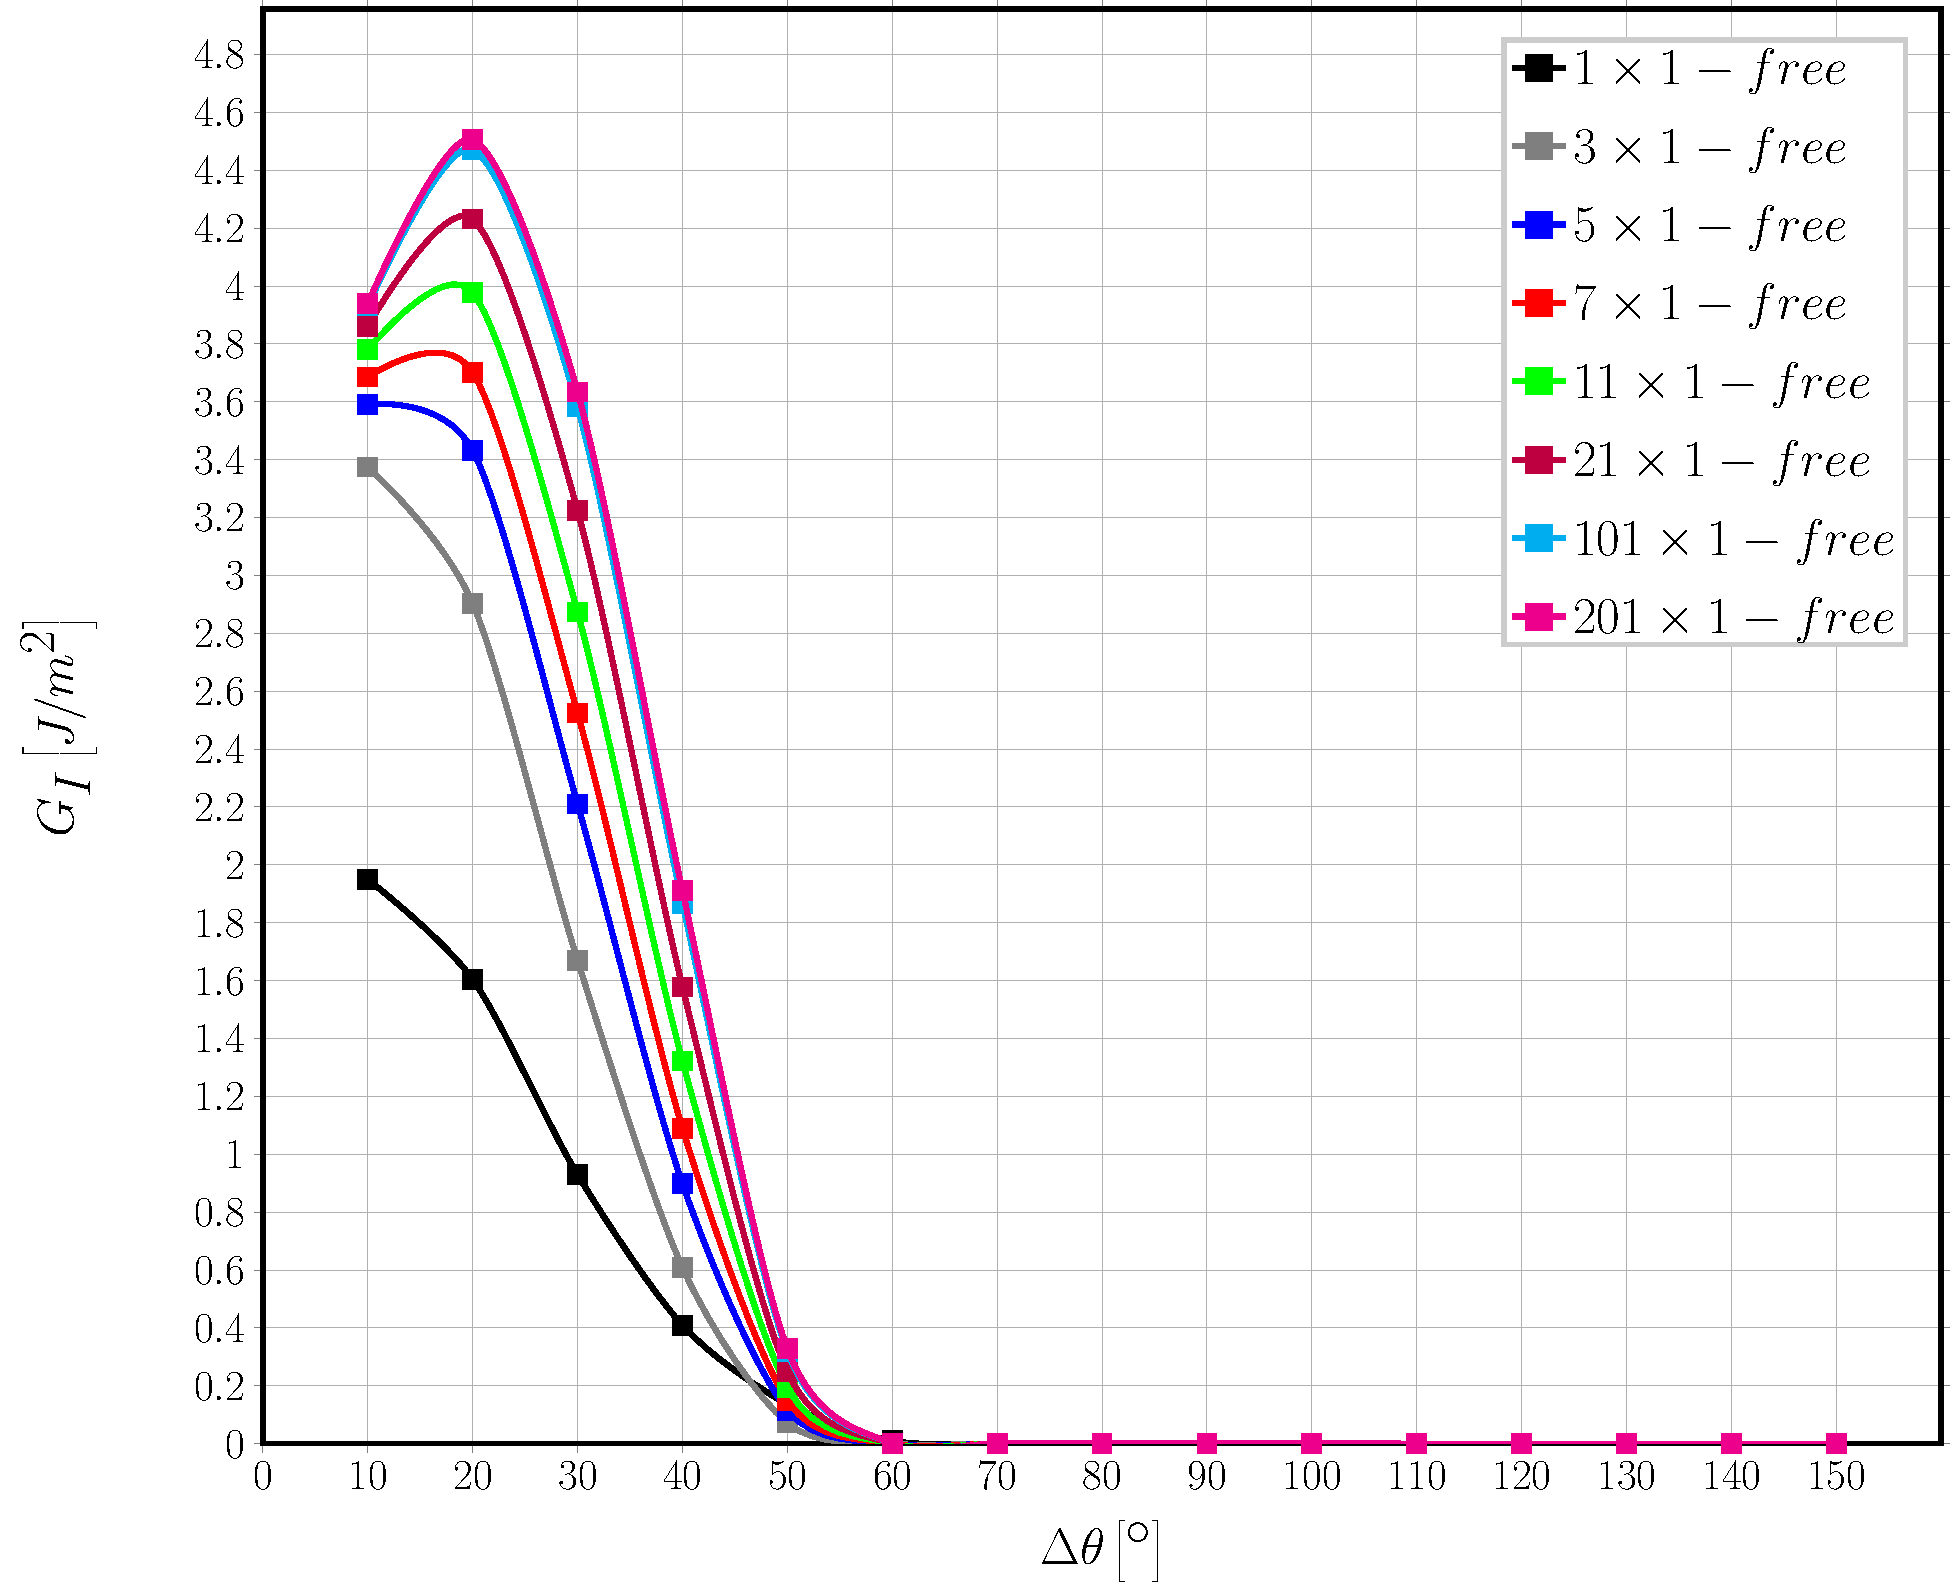
\includegraphics[width=\textwidth]{sidefibers-vf60-GI.pdf}
        \caption{$V_{f}=60\%$.}\label{subfig:sidefiber60MI}
    \end{subfigure}

\caption{Effect of the interaction between debonds appearing at regular intervals on Mode I ERR in an UD with a single layer of fibers at different levels of fiber volume fraction $V_{f}$.}\label{fig:sidefibersMI}
\end{figure}

For Mode I, the presence of a free surface, and inversely the absence of a fully bonded fiber along the vertical direction, implies the absence of the counteracting upward-oriented vertical component of the displacement field due to the mismatch in Poisson's ratios. This in turn translates into the constancy of the value of $\Delta\theta$ corresponding to contact zone's onset, always equal to $60^{\circ}$. For $V_{f}=30\%$, Mode I is reduced going from a debond placed every $5^{th}$ fiber to every $3^{th}$ fiber. Larger spacing does not seem to have a sizable effect. Similarly, at $60\%$ no difference can be seen between the case of a debond placed every $101^{th}$ and every $201^{th}$ fiber. These observations suggest the existence of characteristic distance dependent on the fiber volume fraction which governs the interaction between debonds.

\begin{figure}[!h]
\centering
    \begin{subfigure}[b]{0.475\textwidth}
        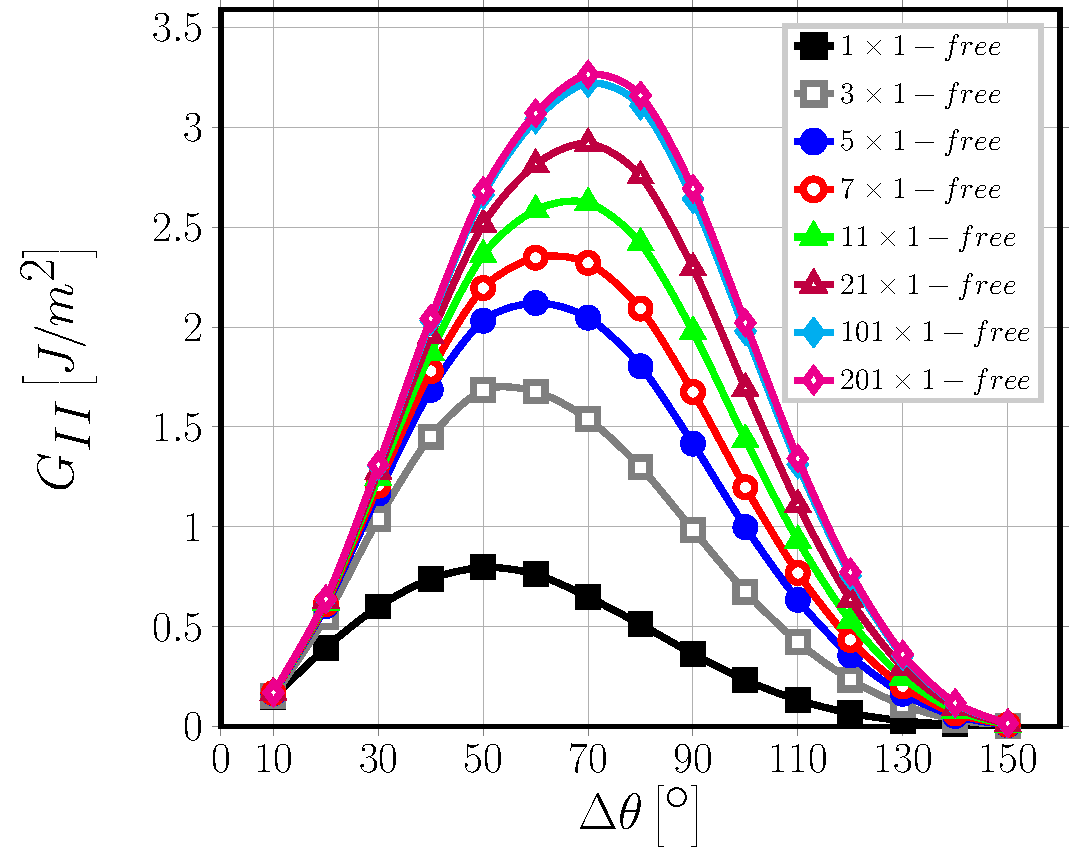
\includegraphics[width=\textwidth]{sidefibers-vf30-GII.pdf}
        \caption{$V_{f}=30\%$.}\label{subfig:sidefiber30MII}
    \end{subfigure} ~
    \begin{subfigure}[b]{0.475\textwidth}
        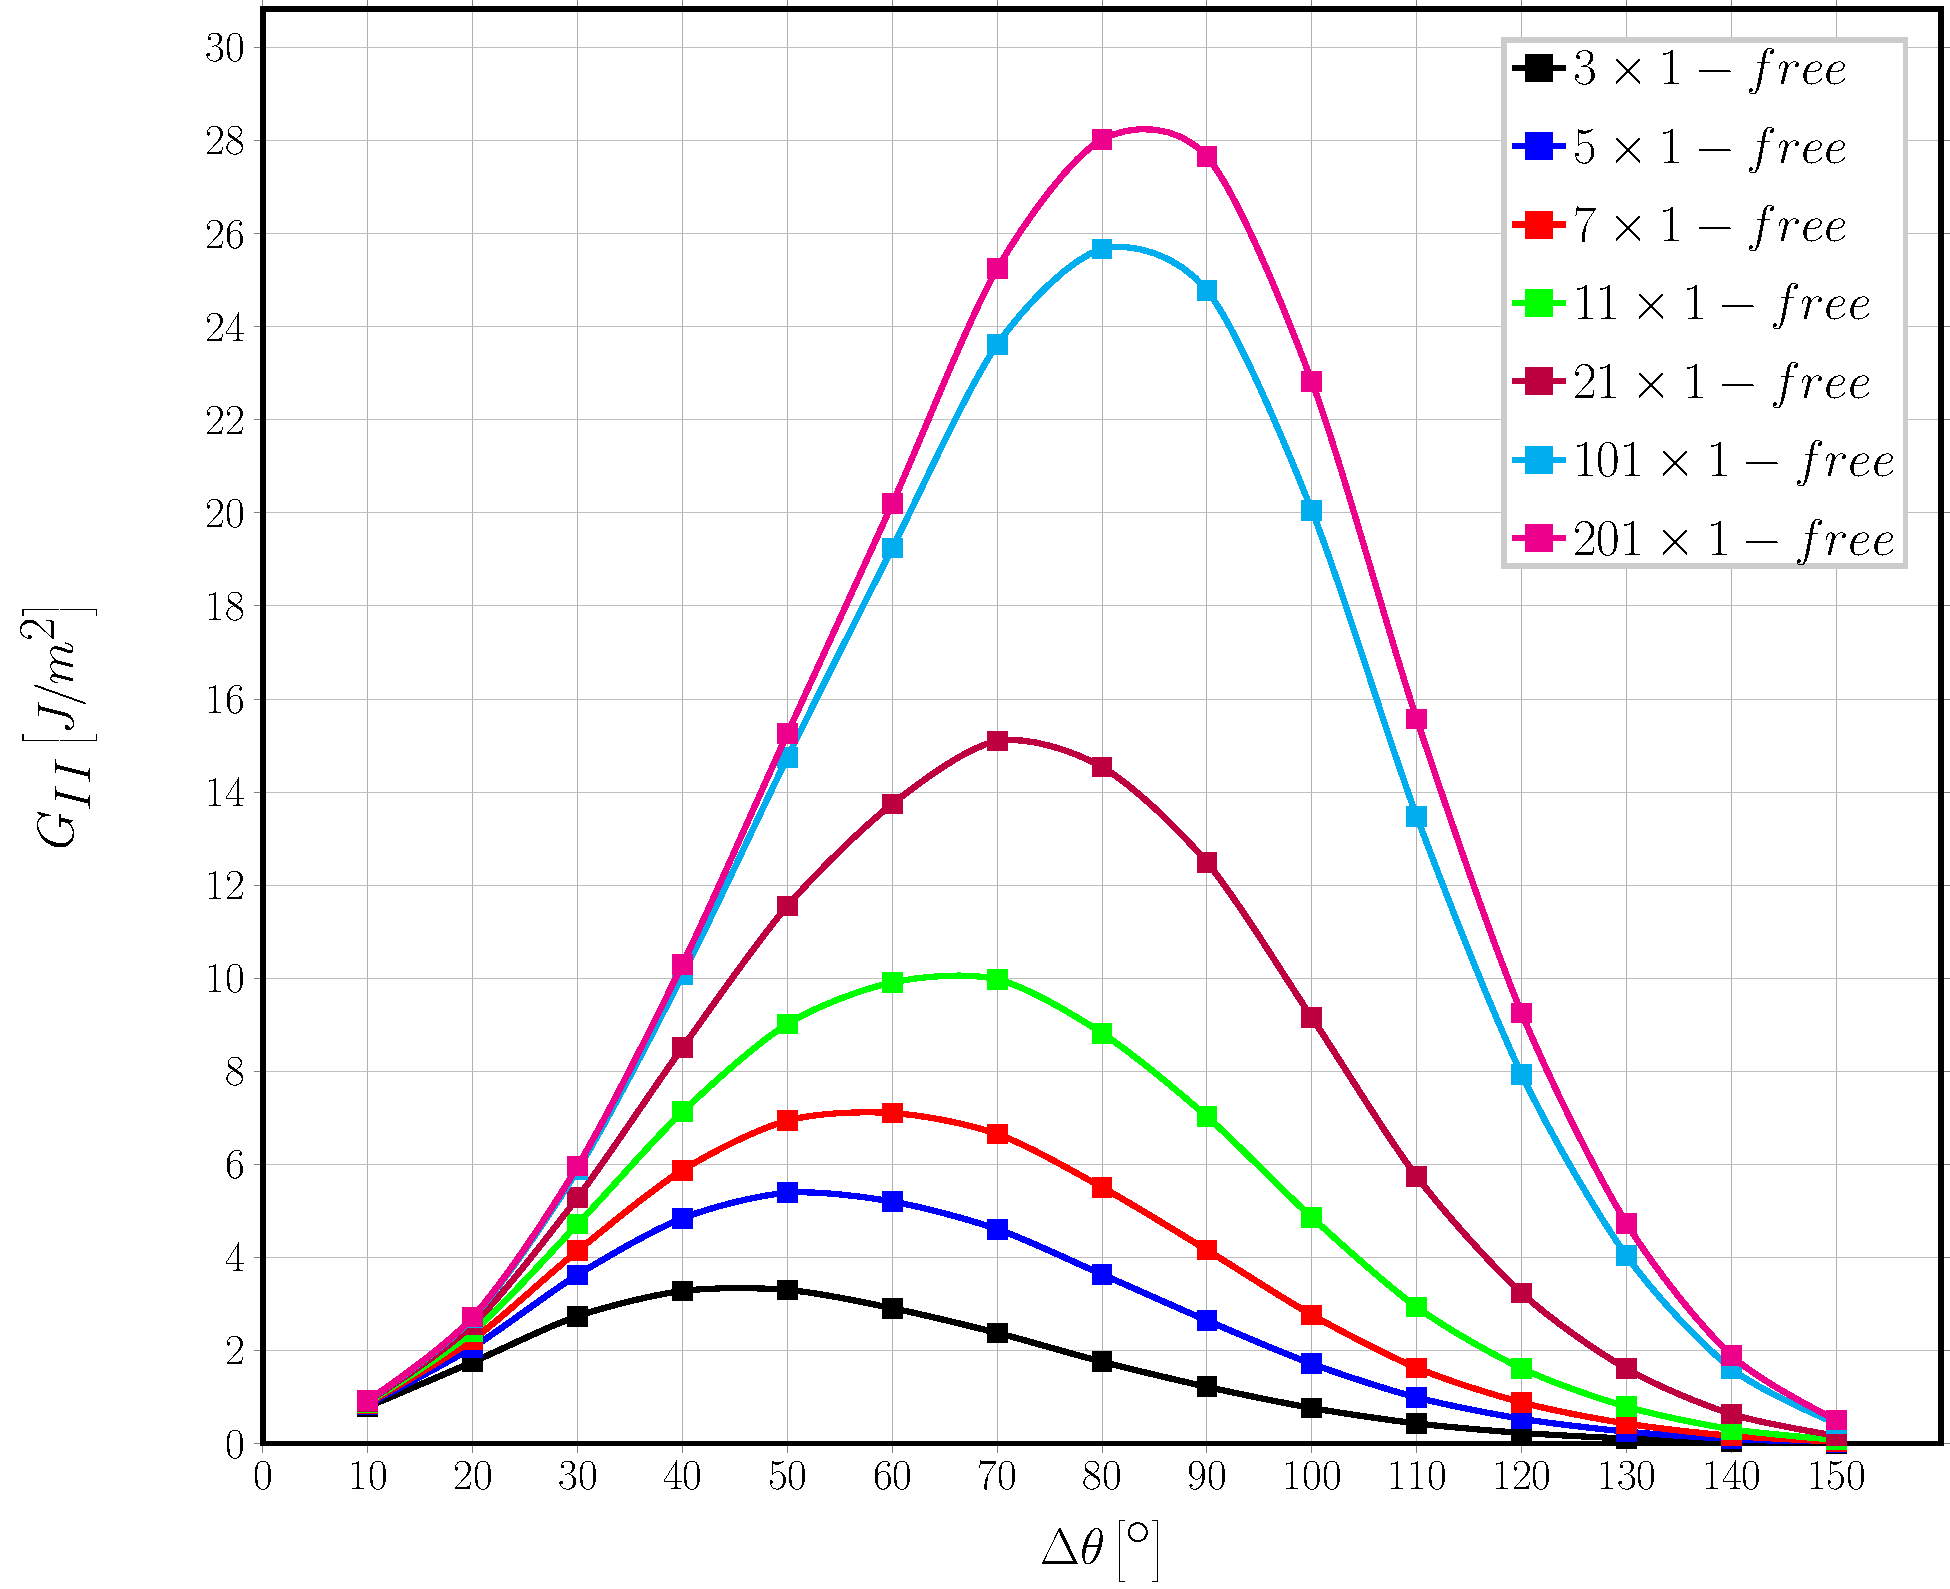
\includegraphics[width=\textwidth]{sidefibers-vf60-GII.pdf}
        \caption{$V_{f}=60\%$.}\label{subfig:sidefiber60MII}
    \end{subfigure}

\caption{Effect of the interaction between debonds appearing at regular intervals on Mode II ERR in a single-ply laminate with a single layer of fibers at different levels of fiber volume fraction $V_{f}$.}\label{fig:sidefibersMII}
\end{figure}

Without costraint on the upper surface, the strain magnification effect creates larger displacements in the x-direction, which increase Mode II for larger debonds. When debonds are far apart, the series of rigid elements (constituted by fully bonded fibers and their sorronding matrix) creates higher x-strains, which in turn generates higher tangential displacements at the crack tip for larger debonds. Conversely, when debonds are closer, the strain concentration is reduced and the tangential component at the crack tip decreases for large $\Delta\theta$. This is the mechanism behind the change in the value of $\Delta\theta$ for which the peak of $G_{II}$ occurs: from $70^{\circ}$ to $50^{\circ}$ at $30\%$, and from $80^{\circ}$ to $40^{\circ}$ at $60\%$ going from the higher to the smaller spacing of debonds. Differently from Mode I, the presence of a characteristic distance is harder to establish. For $V_{f}=30\%$ (Fig.~\ref{subfig:sidefiber30MII}), it seems reasonable to establish it at around 100 fully bonded fibers between each debond. For $V_{f}=60\%$ (Fig.~\ref{subfig:sidefiber60MII}), the difference between models $101\times 1-free$ and $201\times 1-free$ is still sizable, thus preventing the establishment of such characteristic distance. It is possible to observe, however, that the change between $101\times 1-free$ and $201\times 1-free$ is significantly smaller than between $21\times 1-free$ and $101\times 1-free$ ($2\left[\frac{J}{m^{2}}\right]$ vs $11\left[\frac{J}{m^{2}}\right]$), thus suggesting the existence of the characteristic distance outside the range studied.

\subsection{Influence of layers of fully bonded fibers on debond's growth in a line of debonded fibers located at mid-thickness}

The effect of the presence of layers of fully bonded fibers on debond's growth in a line of partially debonded fibers located at mid-thickness in UD composites is studied for Mode I (Fig.~\ref{fig:abovefibersMI}) and Mode II (Fig.~\ref{fig:abovefibersMII}) and fiber content equal to $30\%$ (Figs.~\ref{subfig:abovefiber30MI} and~\ref{subfig:abovefiber30MII}) and $60\%$ (Figs.~\ref{subfig:abovefiber60MI} and~\ref{subfig:abovefiber60MII}). The models treated are $1\times2-free$, $1\times3-free$, $1\times4-free$, $1\times6-free$, $1\times11-free$, $1\times51-free$ and $1\times101-free$, corresponding to a UD composite with respectively $3$, $5$, $7$, $11$, $21$, $101$ and $201$ layers of fibers (Fig.~\ref{subfig:thickplycentraldebonds}).

\begin{figure}[!h]
\centering
    \begin{subfigure}[b]{0.45\textwidth}
        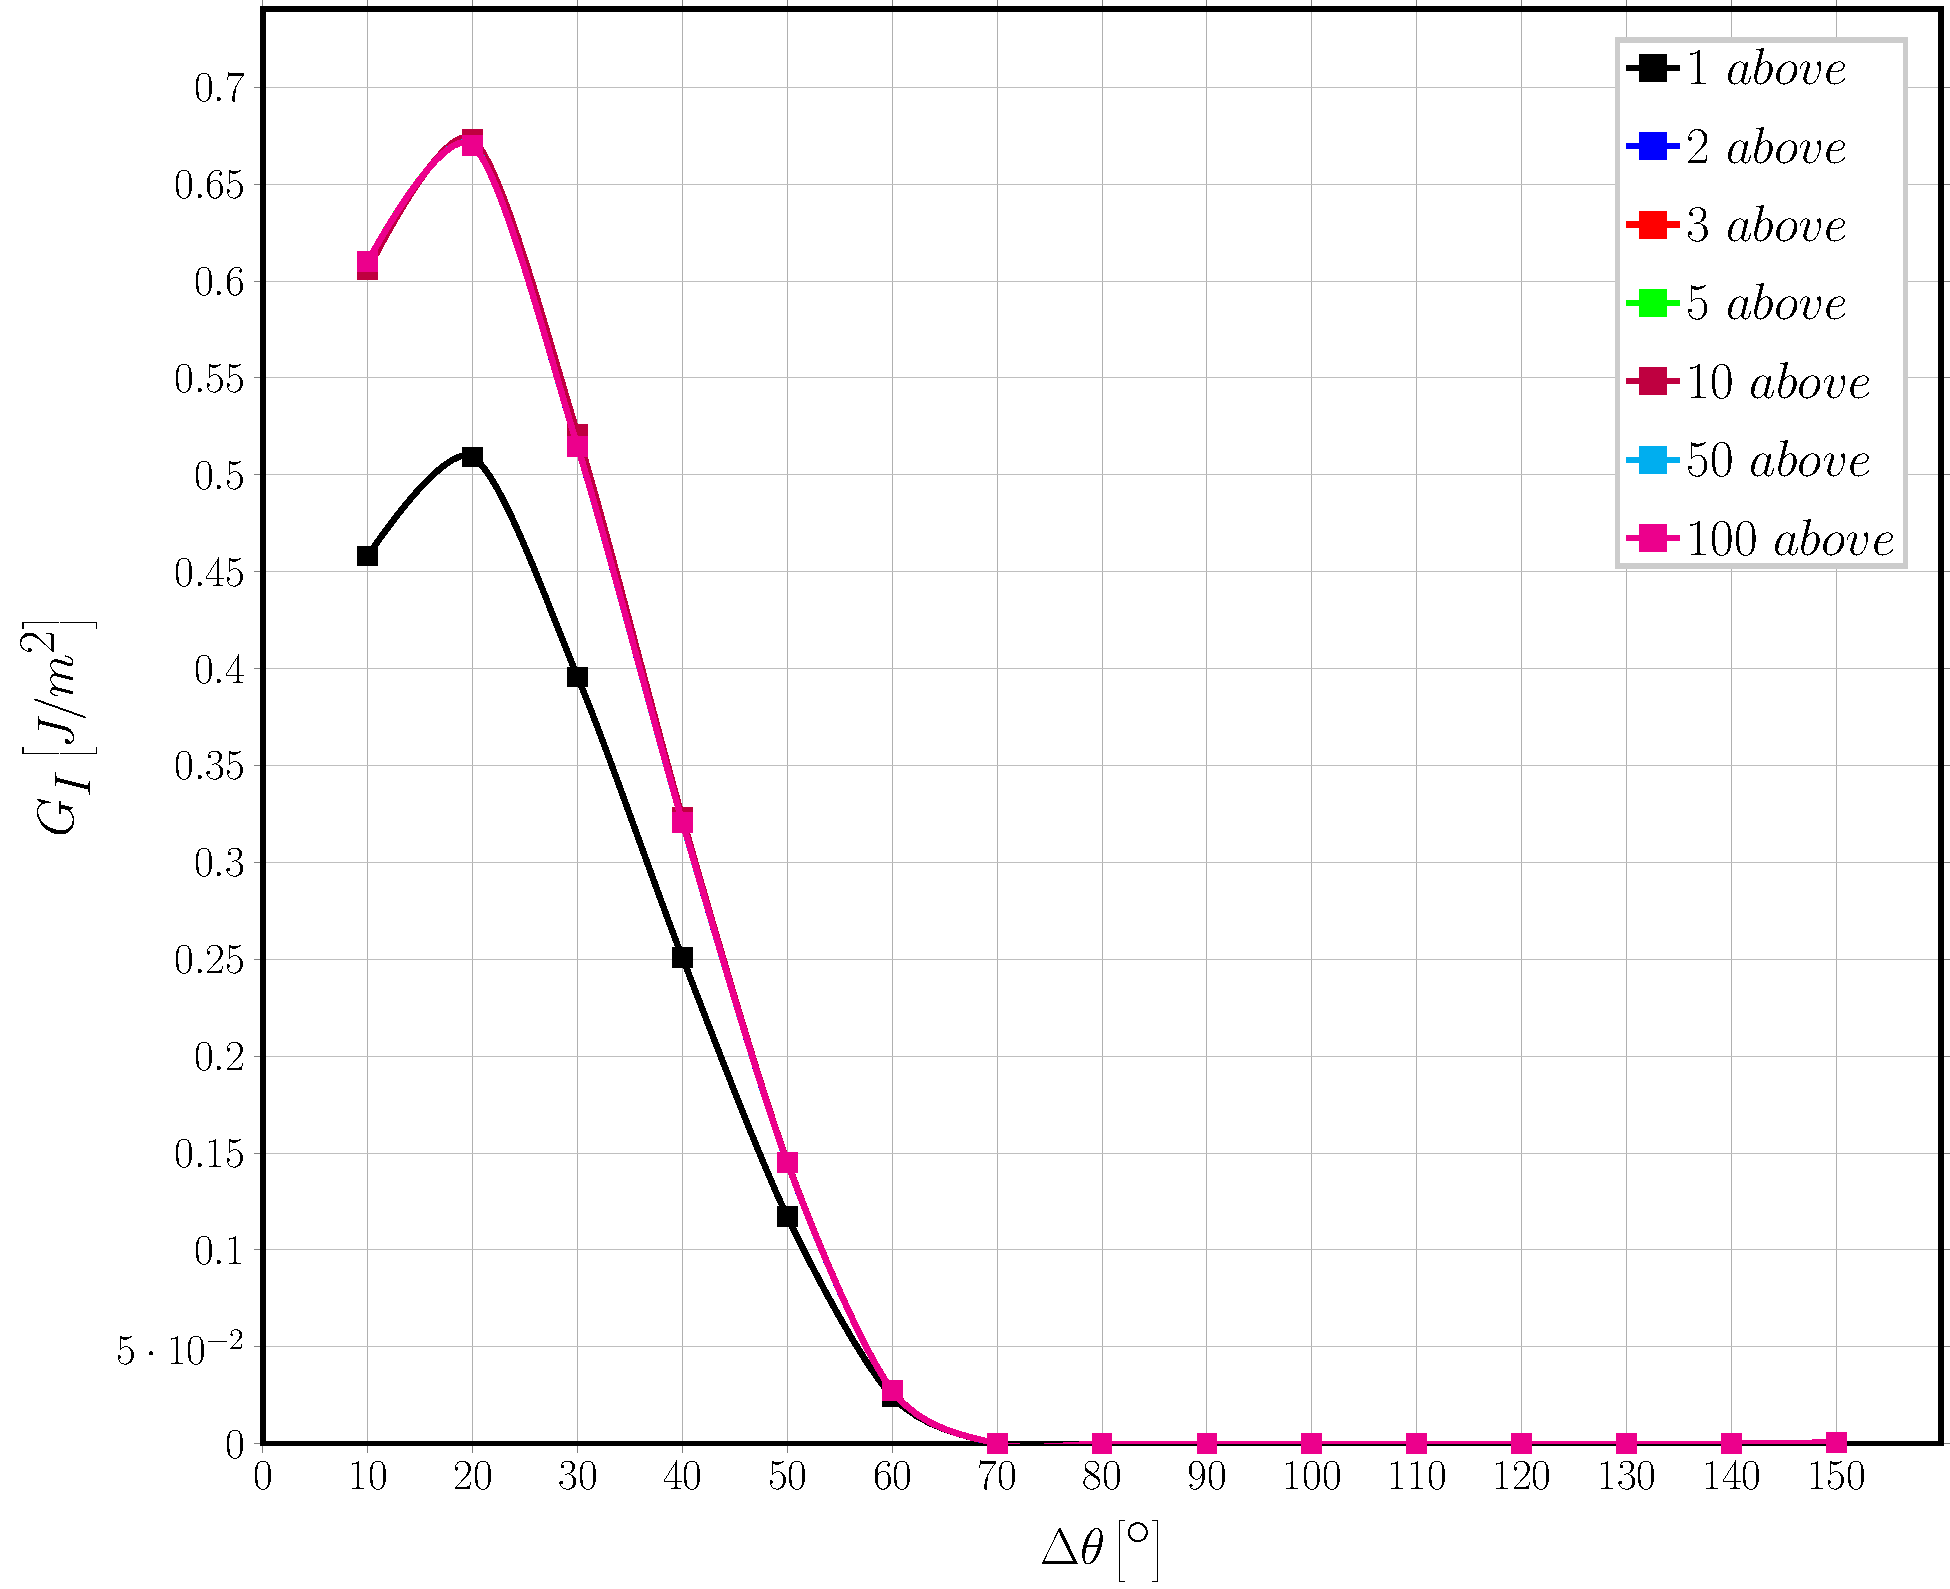
\includegraphics[width=\textwidth]{abovefibers-vf30-GI.pdf}
        \caption{$V_{f}=30\%$.}\label{subfig:abovefiber30MI}
    \end{subfigure} ~
    \begin{subfigure}[b]{0.45\textwidth}
        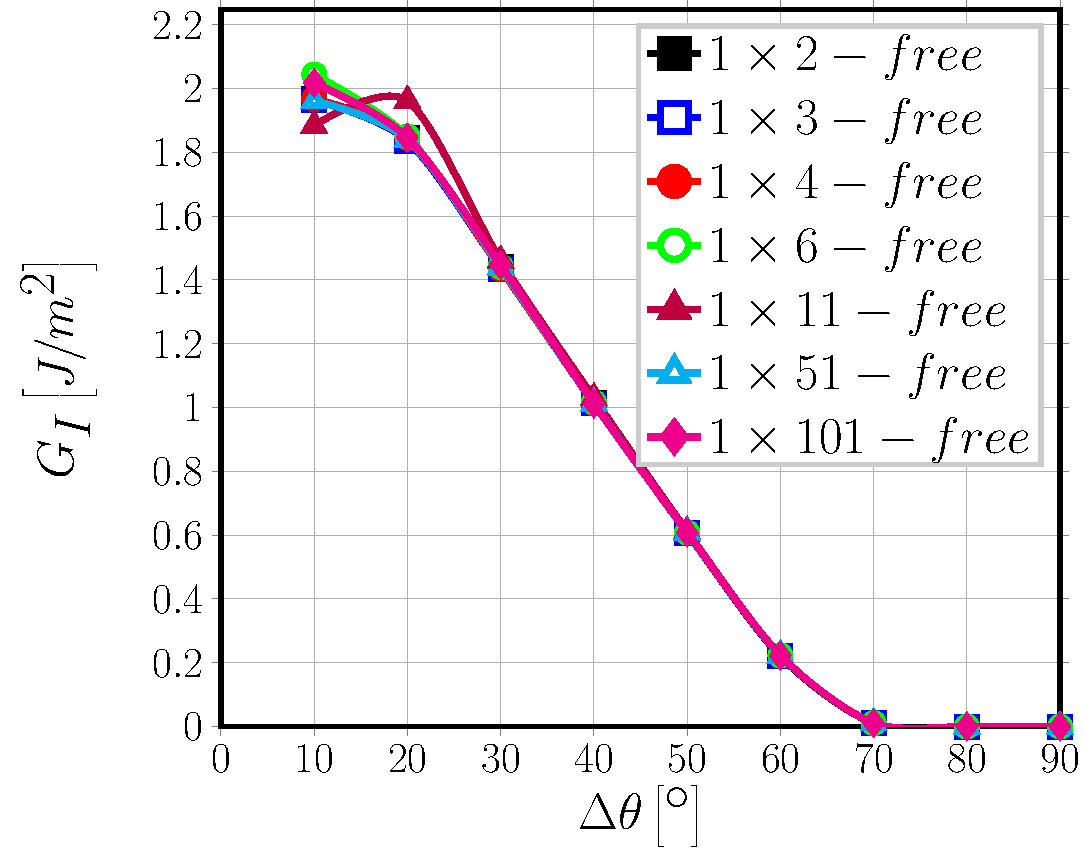
\includegraphics[width=\textwidth]{abovefibers-vf60-GI.pdf}
        \caption{$V_{f}=60\%$.}\label{subfig:abovefiber60MI}
    \end{subfigure}

\caption{Influence of layers of fully bonded fibers on debond's growth in Mode I ERR in a centrally located line of debonded fibers at different levels of fiber volume fraction $V_{f}$.}\label{fig:abovefibersMI}
\end{figure}

The results shown strengthen the considerations made in Sec.~\ref{subsec:volfrac}. It can in fact be seen in Fig.~\ref{fig:abovefibersMI} that the presence of fully bonded fibers across the thickness delays the onset of the contact zone to a debond of $70^{\circ}$ in size, due to the introduction of an additional upward-directed component of the vertical displacement which translates into an opening displacement at the debond's tip.

\begin{figure}[!h]
\centering
    \begin{subfigure}[b]{0.45\textwidth}
        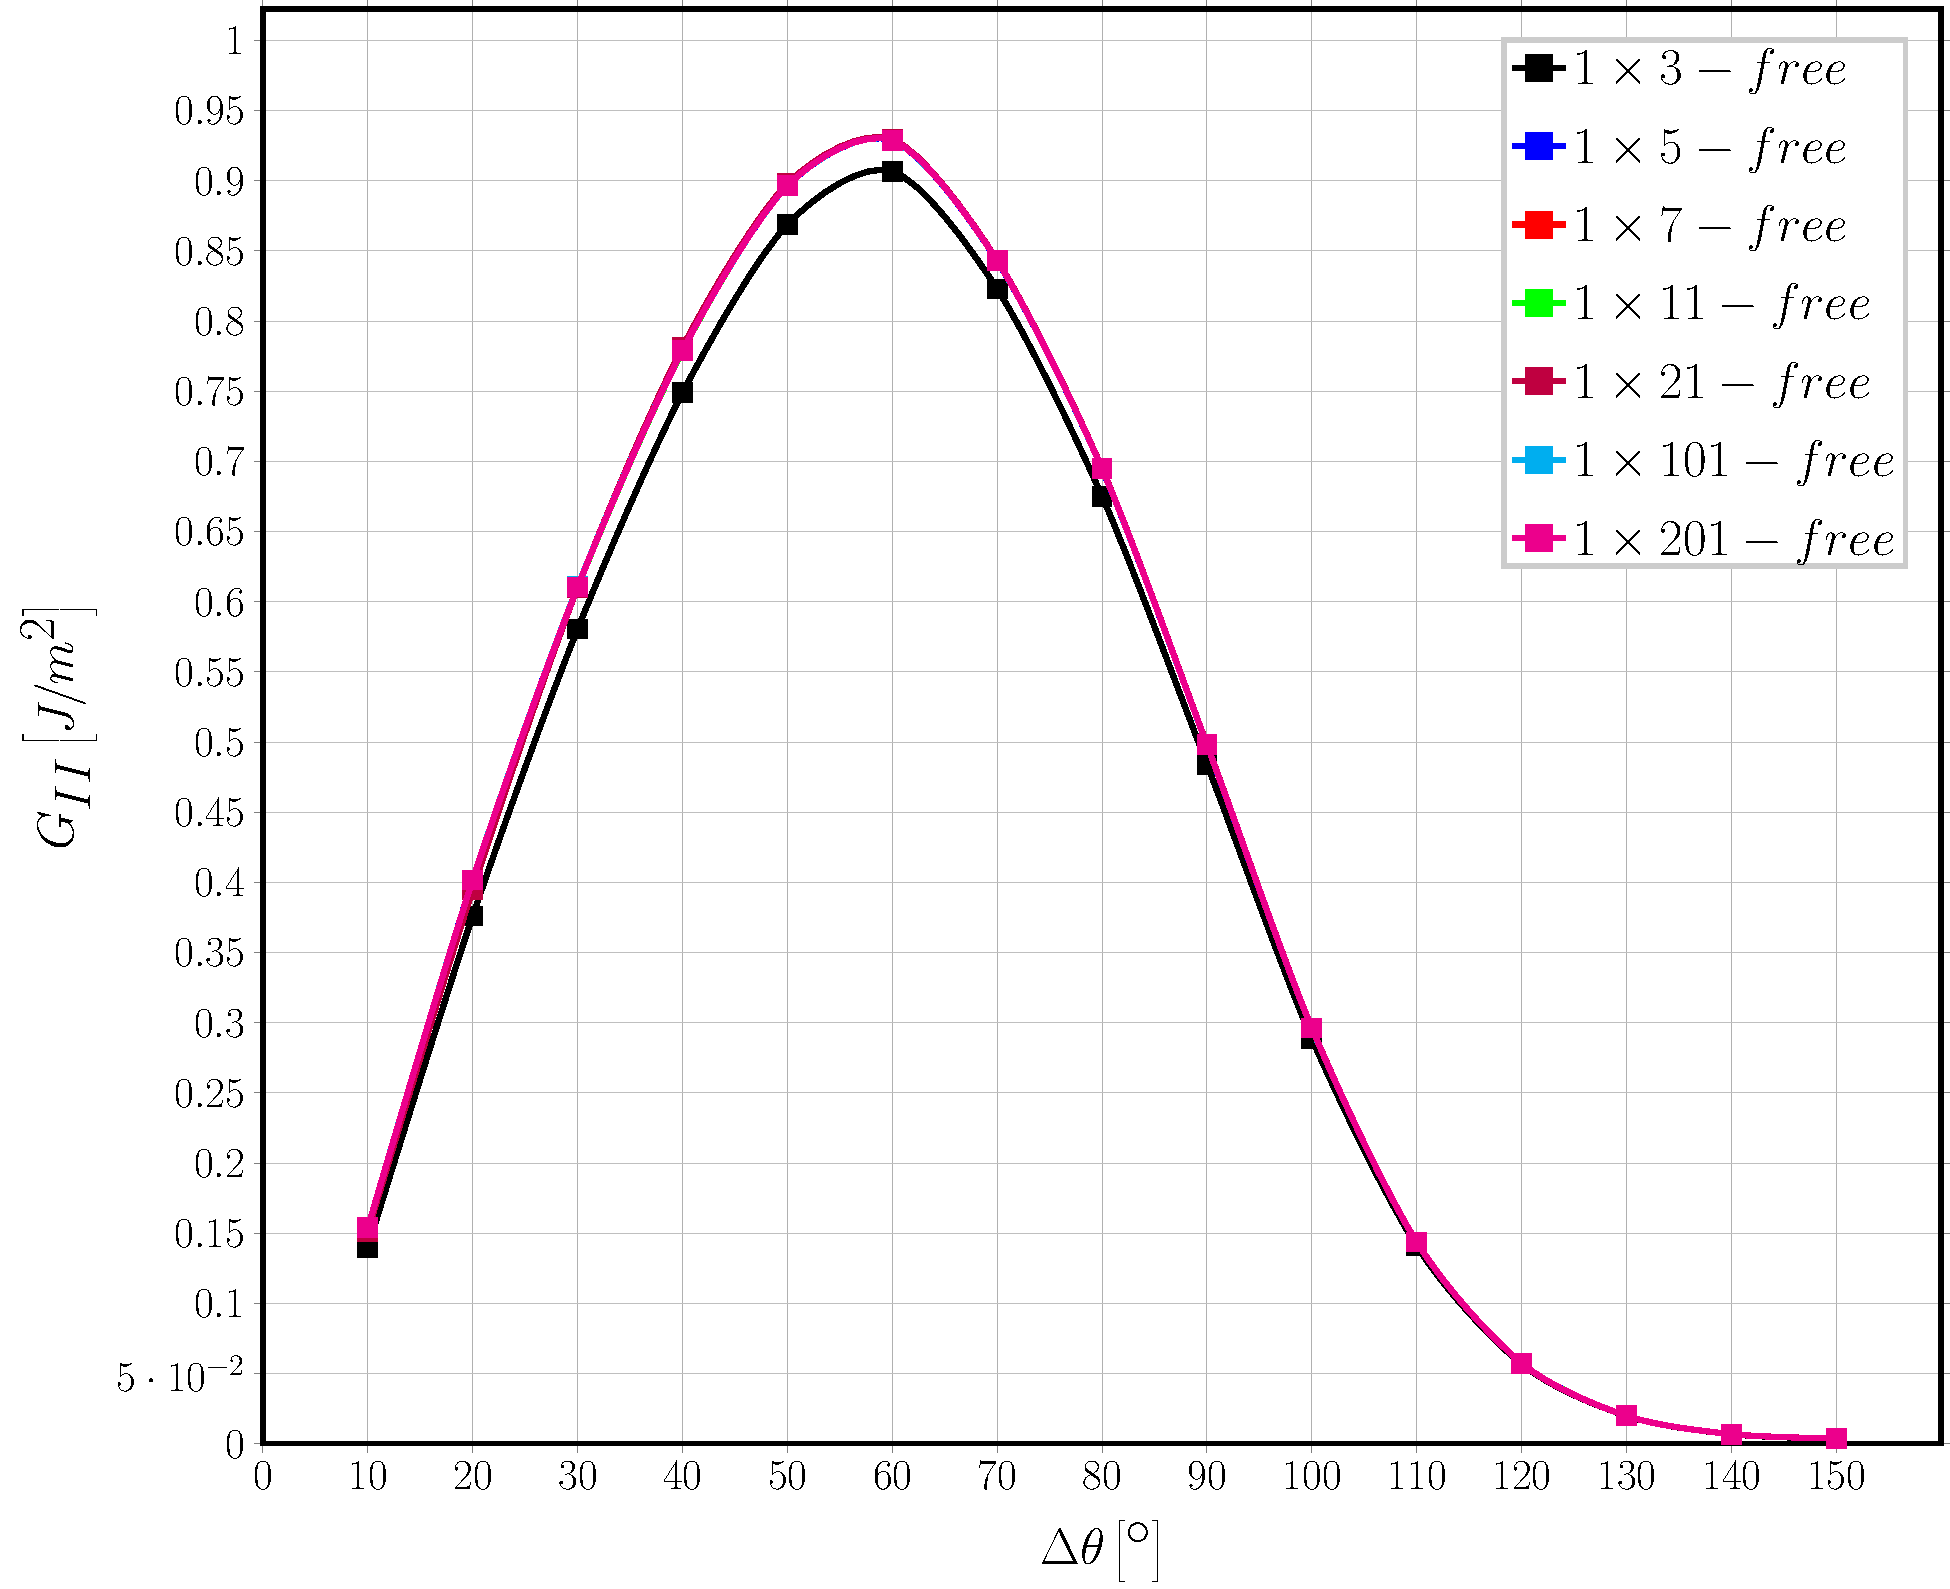
\includegraphics[width=\textwidth]{abovefibers-vf30-GII.pdf}
        \caption{$V_{f}=30\%$.}\label{subfig:abovefiber30MII}
    \end{subfigure} ~
    \begin{subfigure}[b]{0.45\textwidth}
        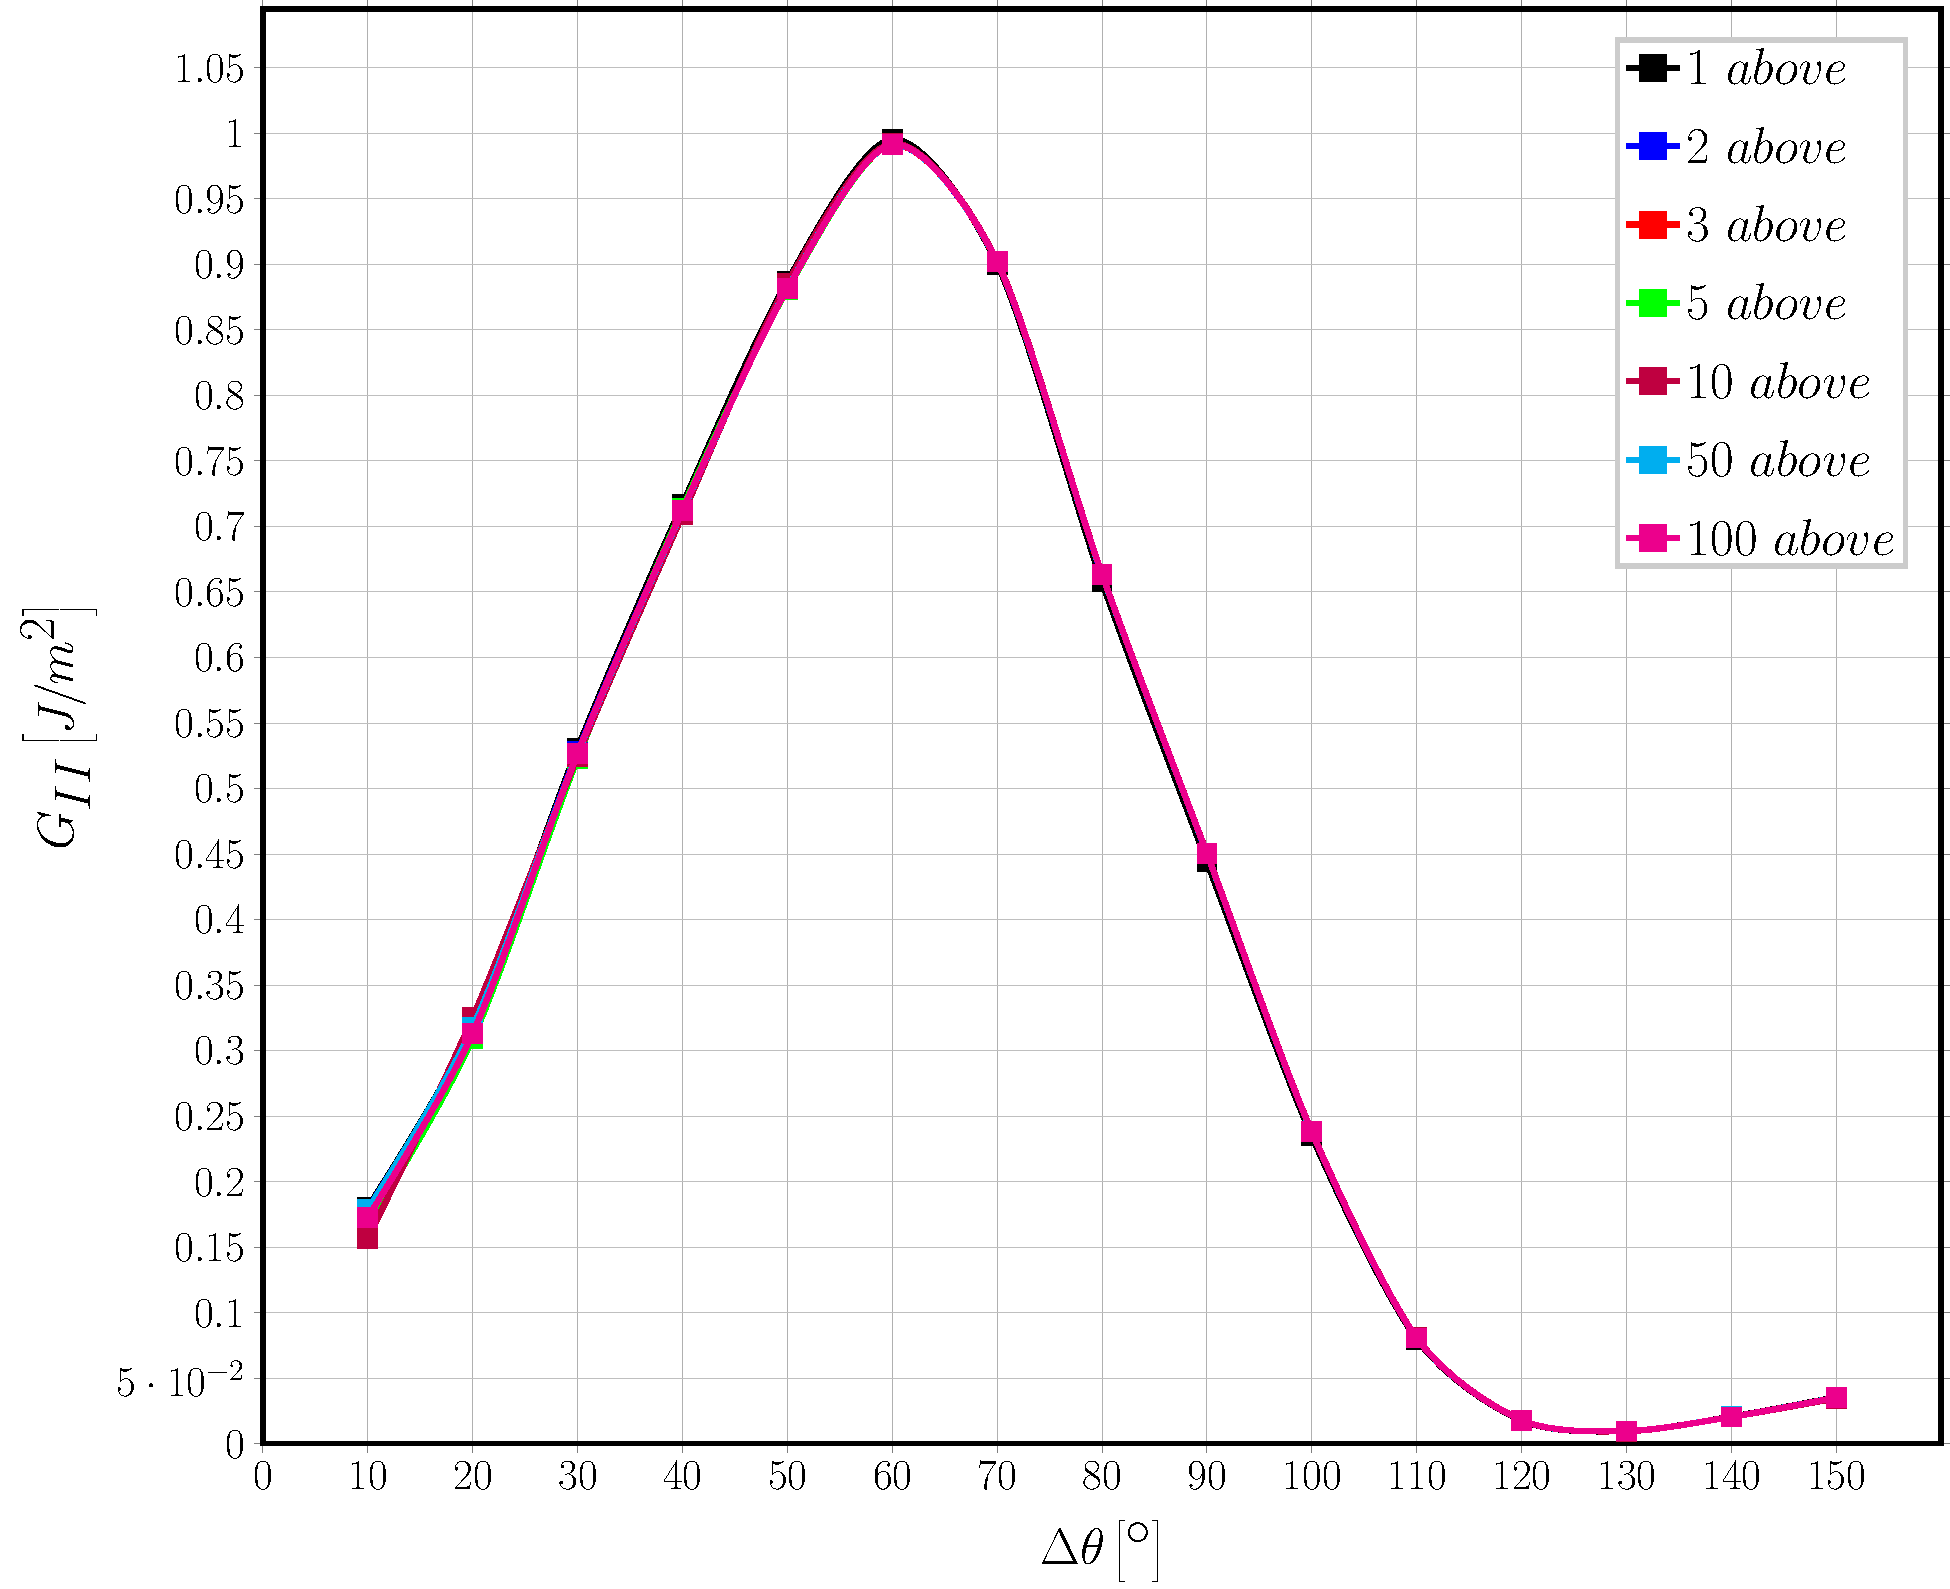
\includegraphics[width=\textwidth]{abovefibers-vf60-GII.pdf}
        \caption{$V_{f}=60\%$.}\label{subfig:abovefiber60MII}
    \end{subfigure}

\caption{Influence of layers of fully bonded fibers on debond's growth in Mode II ERR in a centrally located line of debonded fibers at different levels of fiber volume fraction $V_{f}$.}\label{fig:abovefibersMII}
\end{figure}

The results of both Mode I and Mode II show how the introduction of an increasing number of fully bonded fibers doesn't change the ERR calculated at the crack tip. The effect of the $V_{f}$ can be observed at low fiber content (Figs.~\ref{subfig:abovefiber30MI} and~\ref{subfig:abovefiber30MII}), while for high fiber content the smaller model with only fiber above the partially debonded one is already representative.

\subsection{Interaction between debonds in UD laminates with multiple layers of fibers}

The interaction of debonds appearing at regular intervals in UD composites with multiple layers of fibers is investigated for Mode I (Fig.~\ref{fig:sideabovfibersMI}) and Mode II (Fig.~\ref{fig:sideabovefibersMII}) and fiber content equal to $30\%$ (Figs.~\ref{subfig:sideabovefiber30MI} and~\ref{subfig:sideabovefiber30MII}) and $60\%$ (Figs.~\ref{subfig:sideabovefiber60MI} and~\ref{subfig:sideabovefiber60MII}). The models treated are $3\times 2-free$, $5\times 1-free$, $5\times 2-free$, $11\times 1-free$, $11\times 6-free$, $21\times 1-free$, $21\times 11-free$, $101\times 1-free$, $101\times 6-free$, $201\times 1-free$ and $201\times 6-free$ (Fig.~\ref{subfig:thickply}).

\begin{figure}[!h]
\centering
    \begin{subfigure}[b]{0.475\textwidth}
        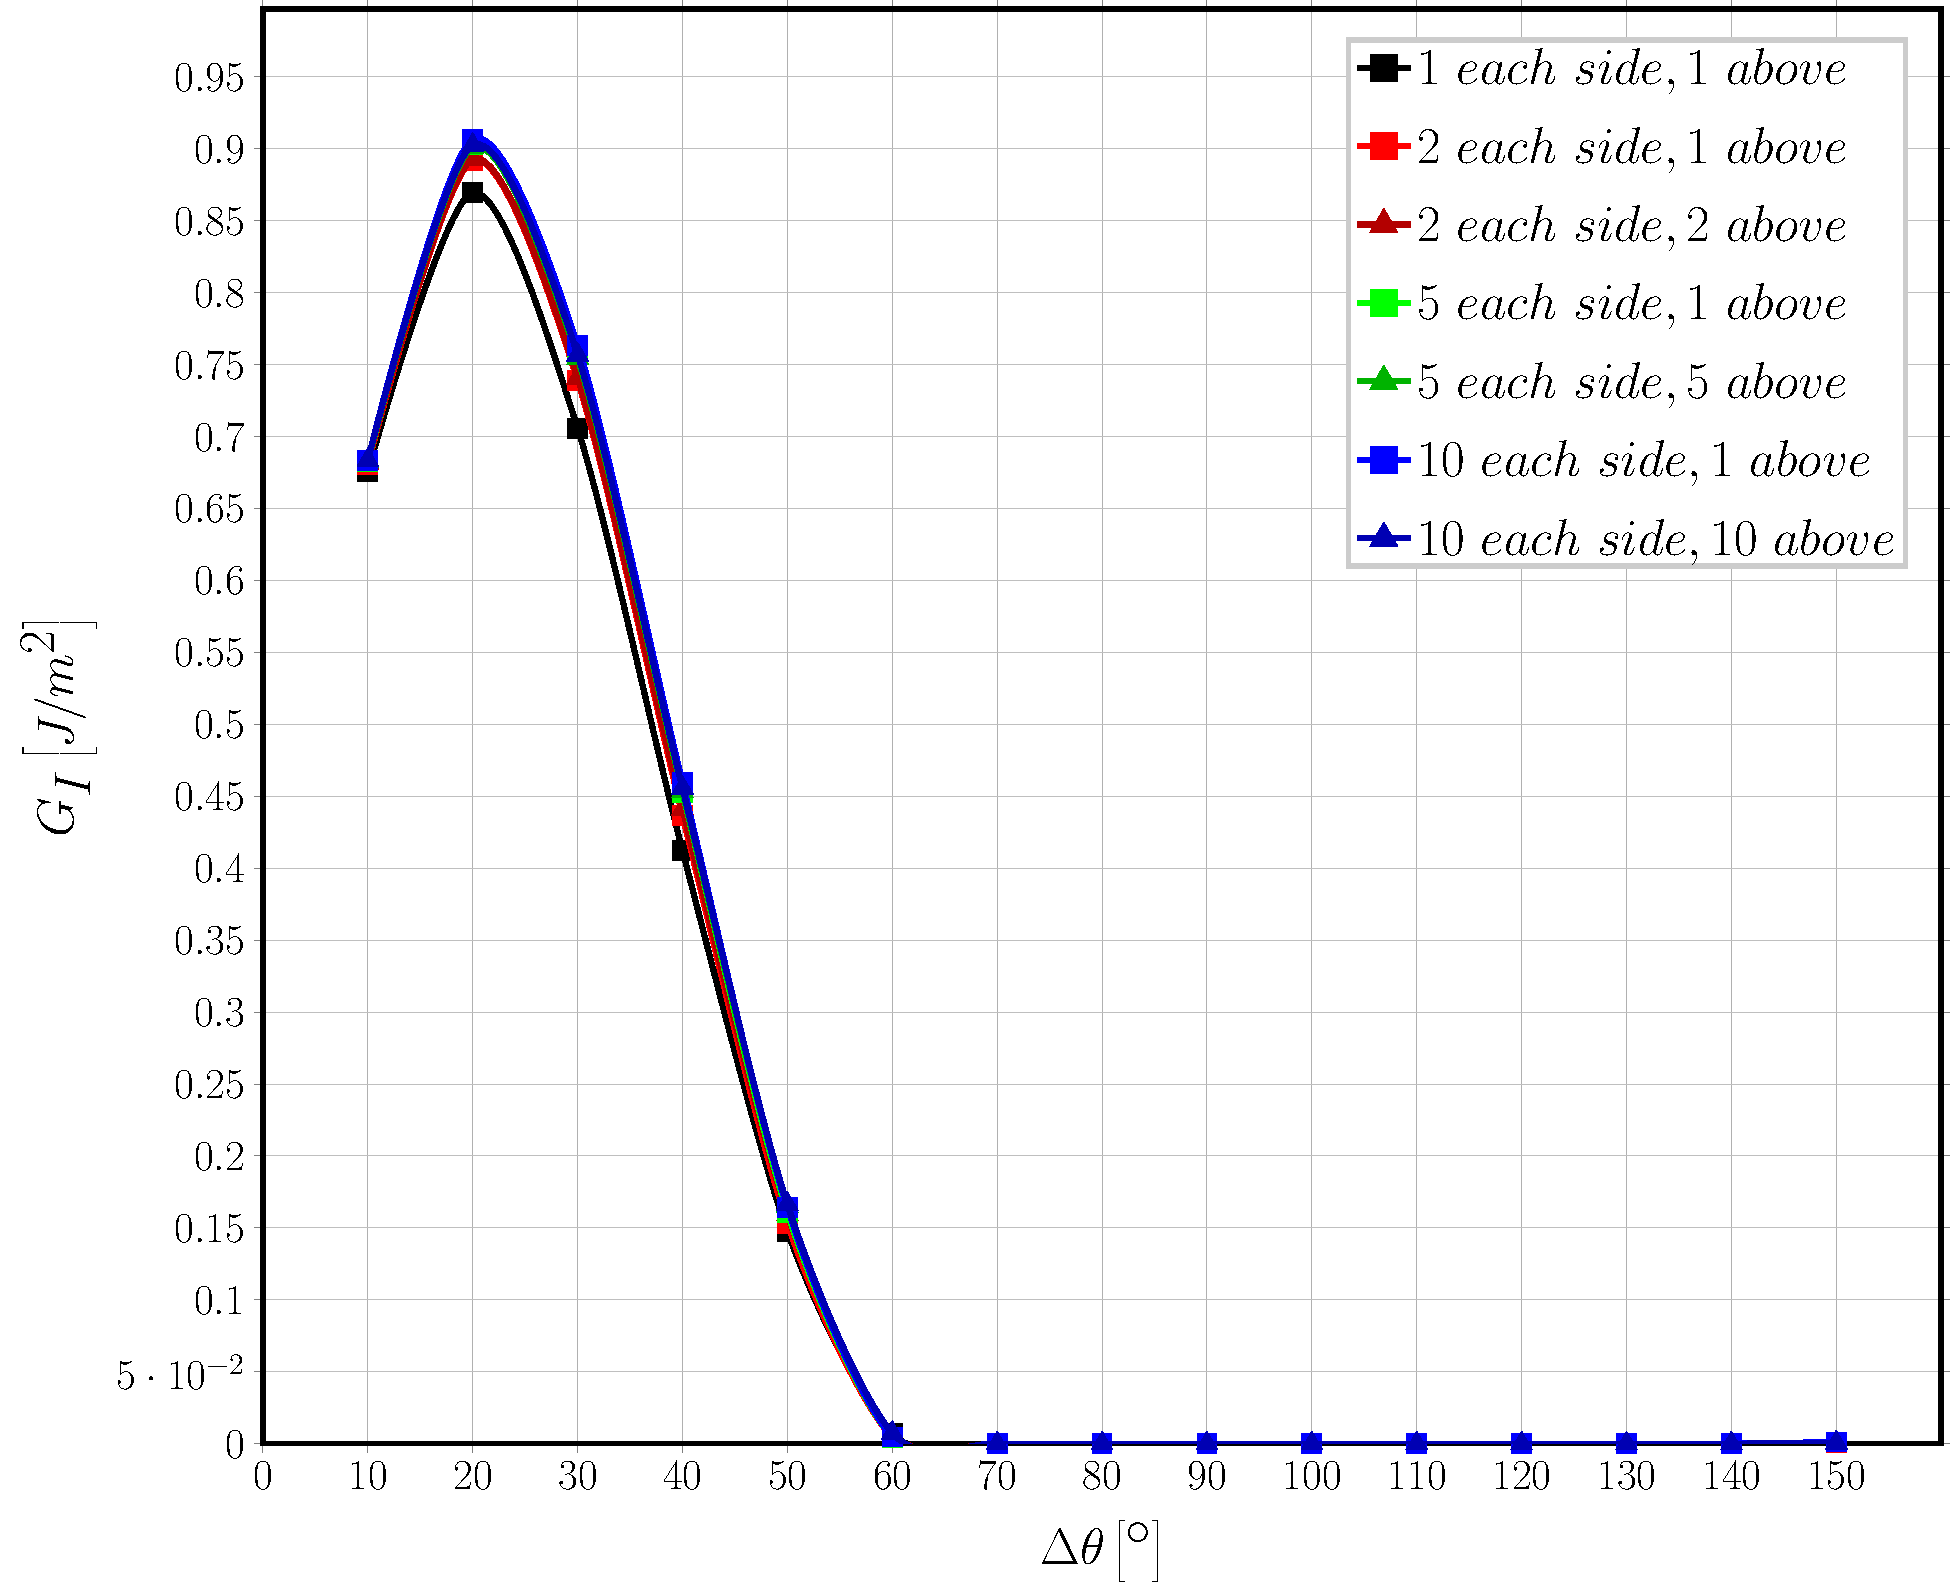
\includegraphics[width=\textwidth]{sideabovefibers-vf30-GI.pdf}
        \caption{$V_{f}=30\%$.}\label{subfig:sideabovefiber30MI}
    \end{subfigure} ~
    \begin{subfigure}[b]{0.475\textwidth}
        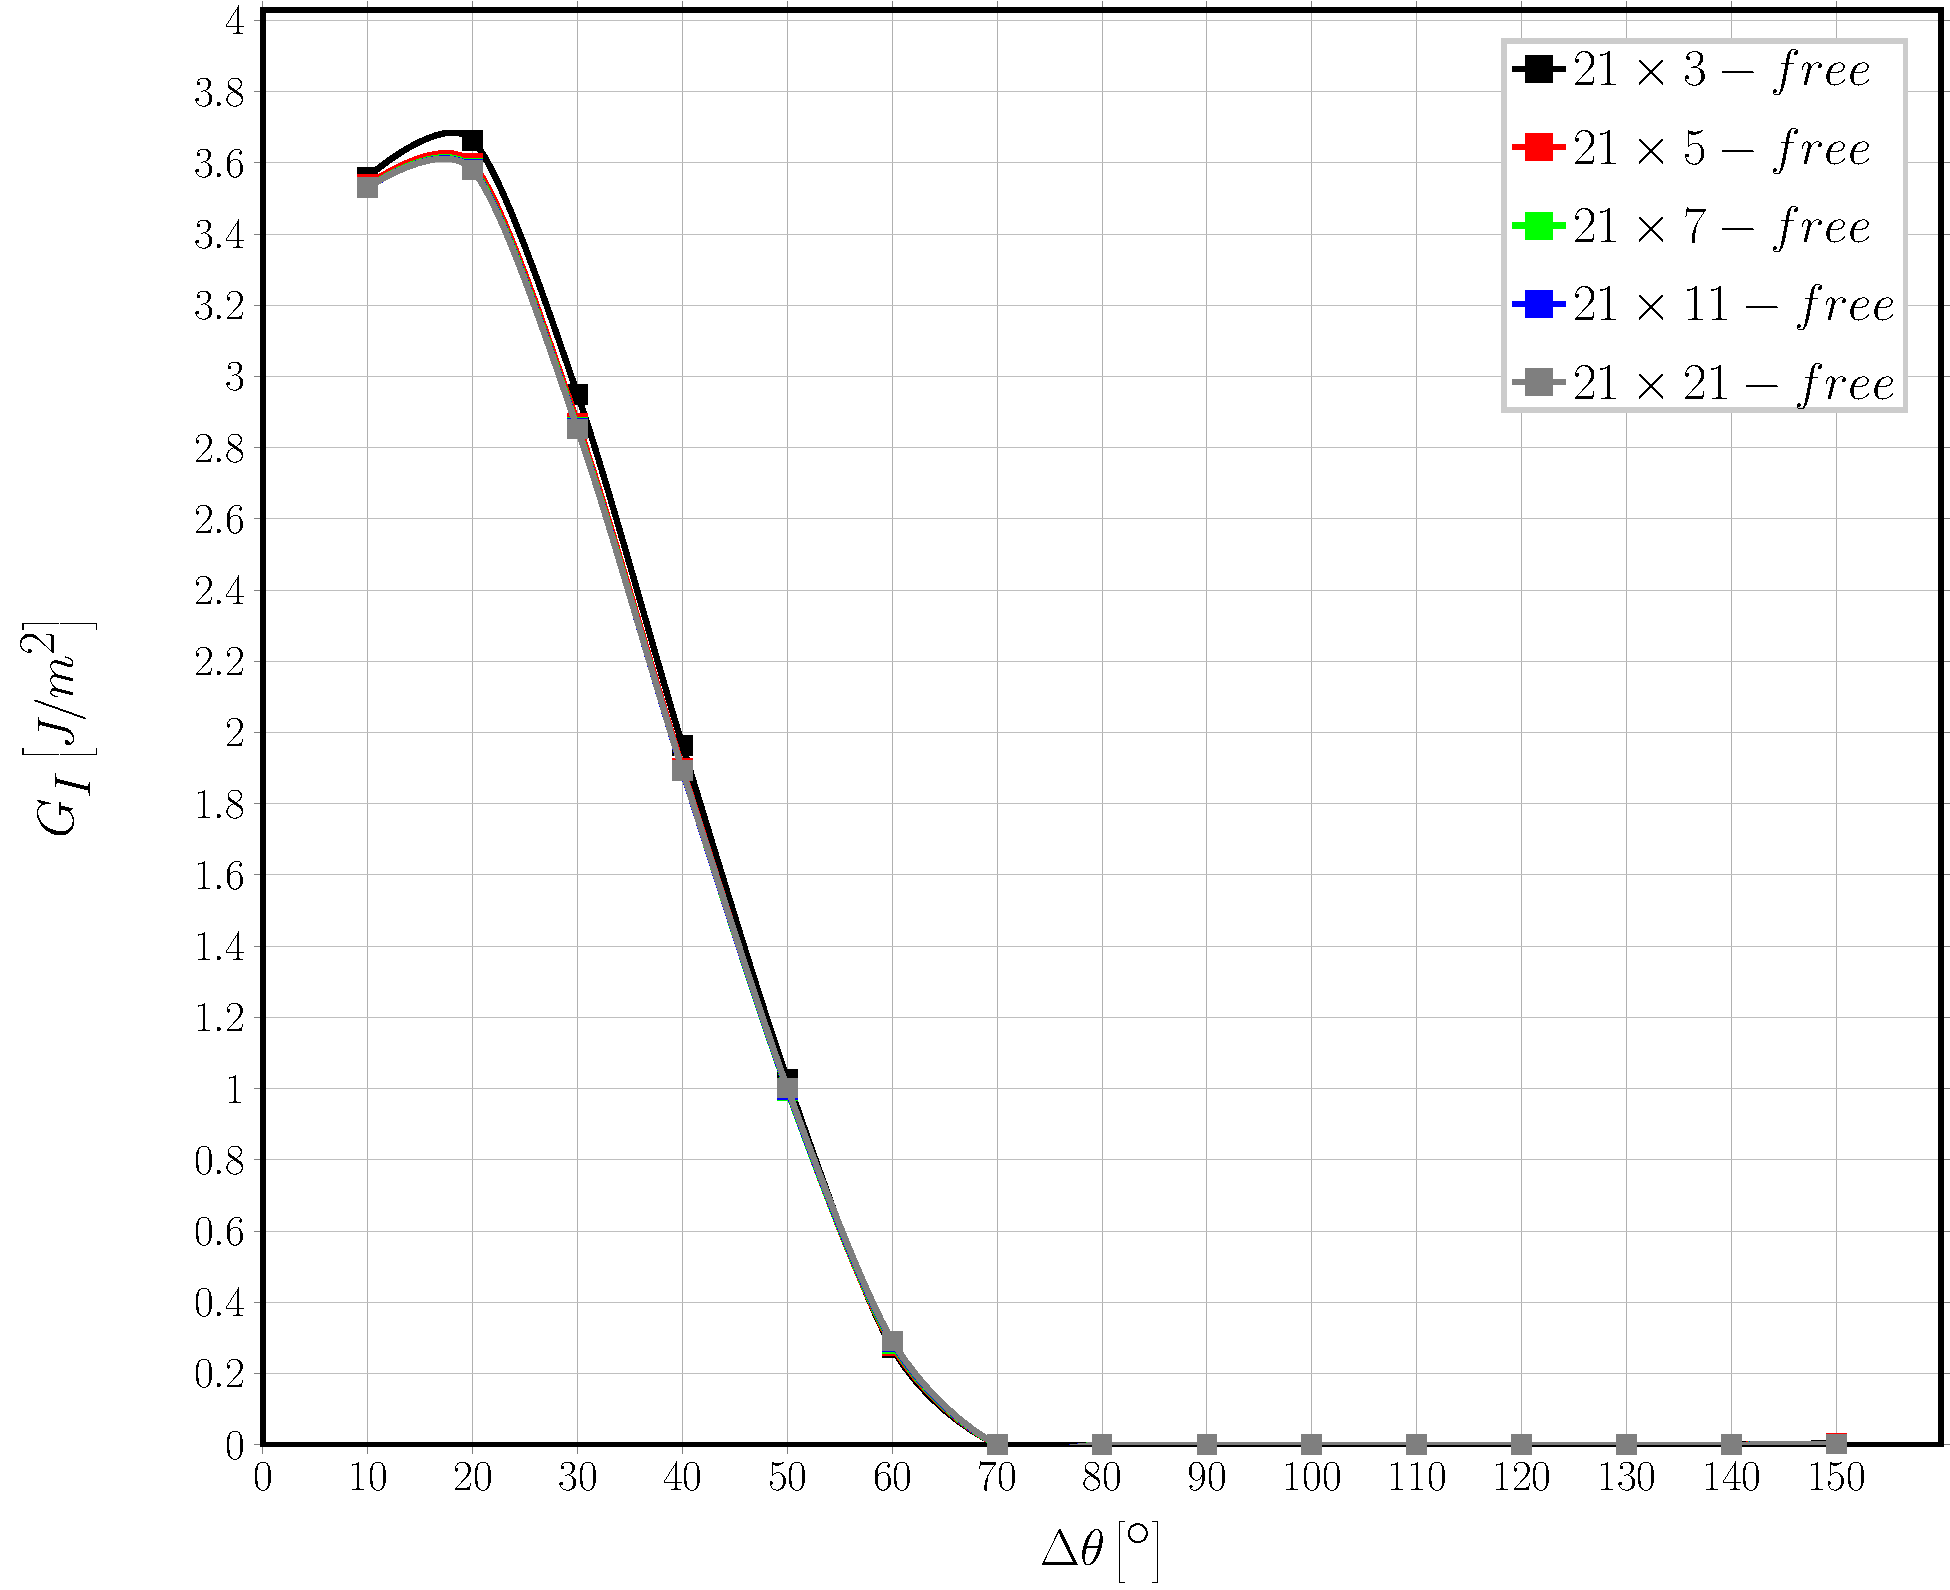
\includegraphics[width=\textwidth]{sideabovefibers-vf60-GI.pdf}
        \caption{$V_{f}=60\%$.}\label{subfig:sideabovefiber60MI}
    \end{subfigure}

\caption{Effect of the interaction between debonds appearing at regular intervals on Mode I ERR in a single-ply laminate with multiple layers of fibers at different levels of fiber volume fraction $V_{f}$.}\label{fig:sideabovefibersMI}
\end{figure}

Comparing with the results in Sec.~\ref{subsec:singlefiberud}, it can be observed how the presence of fully bonded fibers across the thickness has a restraining effect on the ERR, that counteracts the magnification due to an increasing number of fully bonded fibers in the horizontal direction. The interplay is further modulated by the fiber content. For Mode I, at low fiber content the contact zone onset starts at $60^{\circ}$, while it is delayed to debonds of $70^{\circ}$ for $V_{f}=60\%$. Convergence can also be observed: at $30\%$ fiber volume fraction, the $5\times 2-free$ model can already be considered representative of further spaced debonds in arbitrarily thick UDs; at $60\%$, the $21\times 2-free$ model can be considered representative of laminates with 3 layers of fibers and the $11\times 6-free$ of thicker UDs. A less definite situation characterizes instead Mode II. An increase in the value of ERR can be observed for any additional fully bonded fiber present in the horizontal direction, while a change due to the number of fibers across the thickness can be observed only between $1$ and $>1$.

\begin{figure}[!h]
\centering
    \begin{subfigure}[b]{0.475\textwidth}
        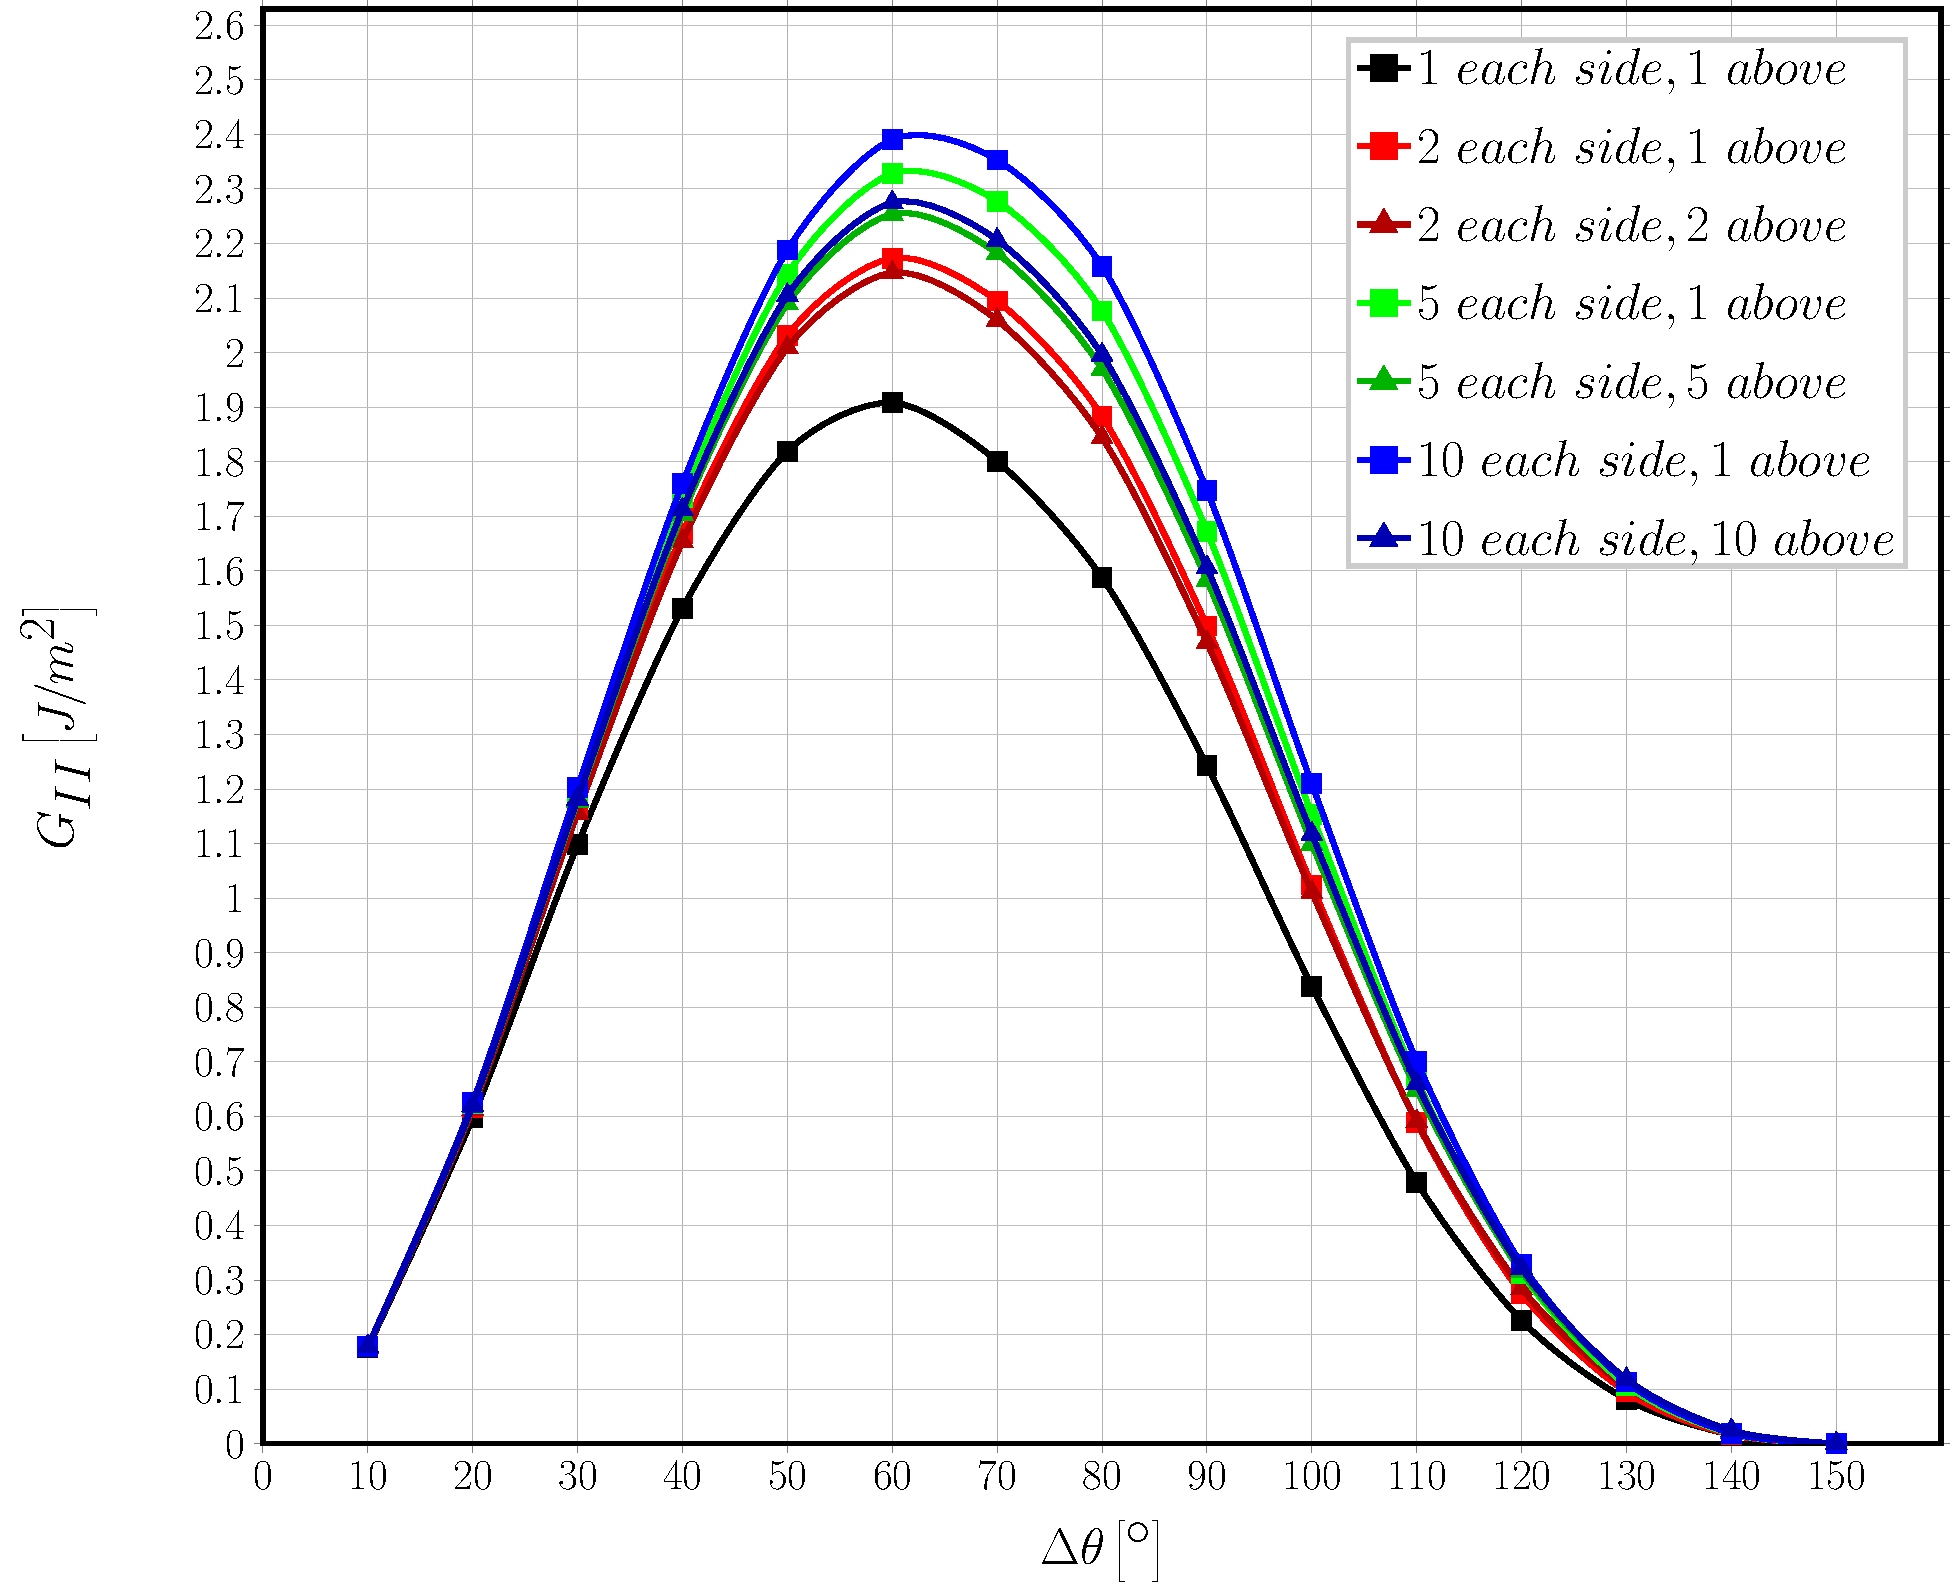
\includegraphics[width=\textwidth]{sideabovefibers-vf30-GII.pdf}
        \caption{$V_{f}=30\%$.}\label{subfig:sideabovefiber30MII}
    \end{subfigure} ~
   \begin{subfigure}[b]{0.475\textwidth}
        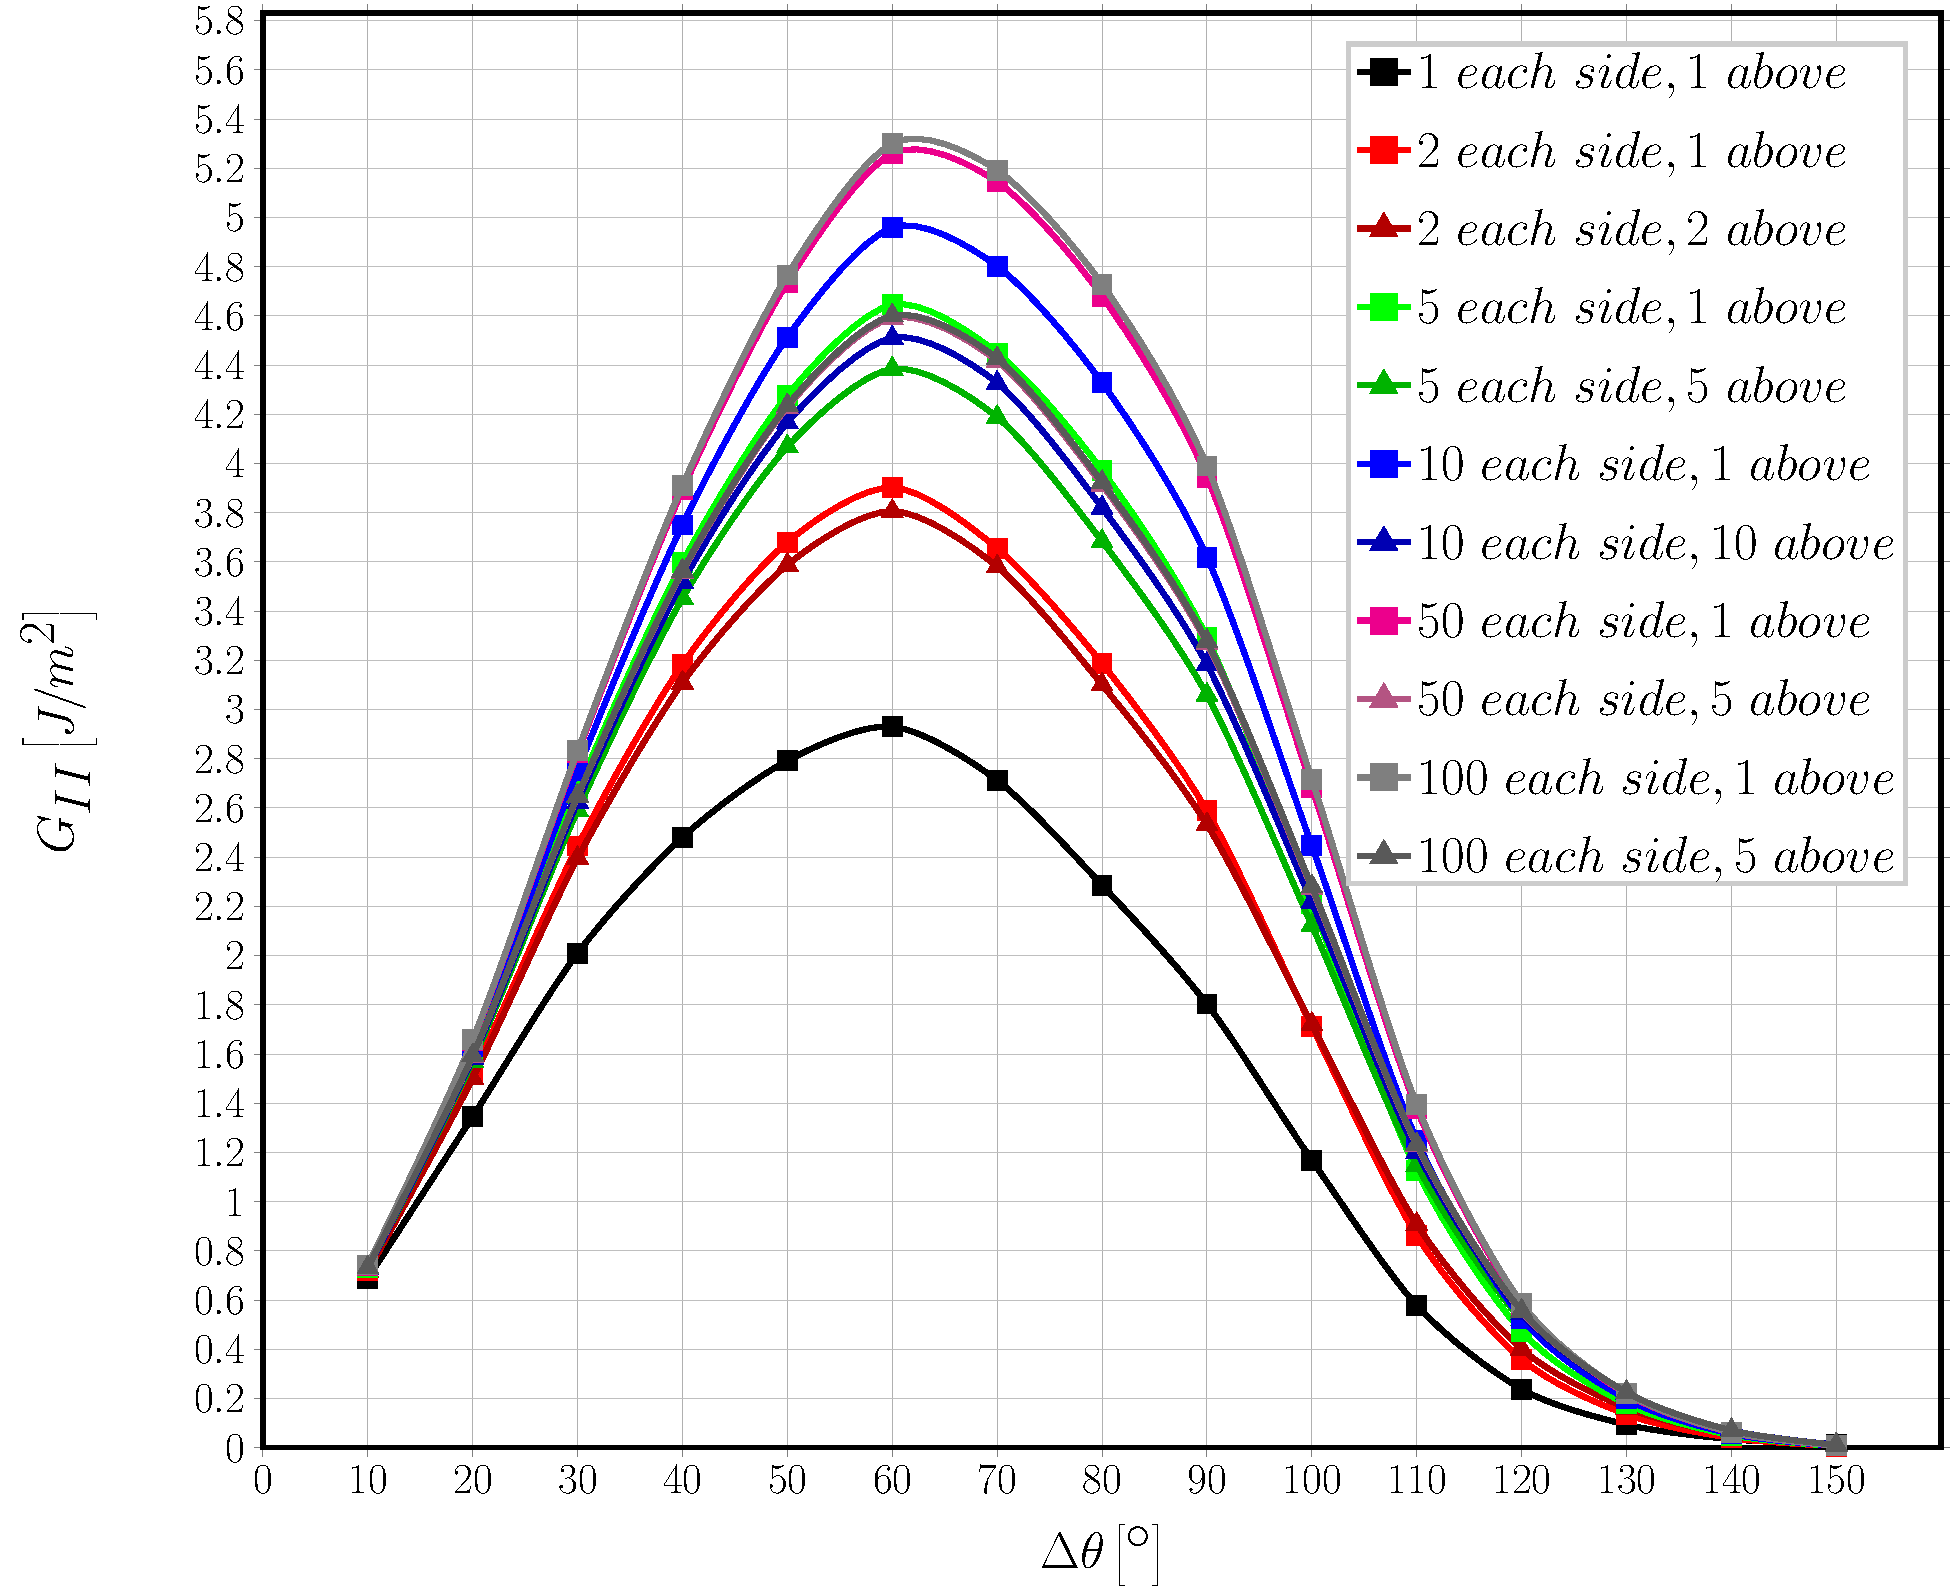
\includegraphics[width=\textwidth]{sideabovefibers-vf60-GII.pdf}
        \caption{$V_{f}=60\%$.}\label{subfig:sideabovefiber60MII}
    \end{subfigure}

\caption{Effect of the interaction between debonds appearing at regular intervals on Mode II ERR in a single-ply laminate with multiple layers of fibers at different levels of fiber volume fraction $V_{f}$.}\label{fig:sideabovefibersMII}
\end{figure}

It seems to be apparent that the interaction of debonds is strongly affected by the presence of fully bonded fiber between them: the further apart debonds are, the higher the Energy Release Rate. The presence of layers of fully bonded fibers has instead a suppressing effect and there exists a limit value of layers after which no sizeable change is measurable. Such limit value seems however to depend on the spacing of debonds in the horizontal direction. Increasing the fiber content leads in general to more drastic changes in the ERR.

\subsection{Comparison with the single fiber model with equivalent boundary conditions}

The comparison of the single fiber models with the corresponding multi-fiber models (Figs.~\ref{fig:comparisonfreeMI},~\ref{fig:comparisonfreeMII},~\ref{fig:comparisonfreeMI} and~\ref{fig:comparisonfreeMII}) show that the former provide in general the lowest estimation of the ERR and correspond to the most damaged state of the laminate, i.e. the state in which the greatest number of debonds is present. The $1\times 1-free$ or simply free model (Figs.~\ref{fig:comparisonfreeMI} and~\ref{fig:comparisonfreeMII}), which represents a UD with a single layer of partially debonded fibers, agrees with the results of Sec.~\ref{subsec:singlefiberud} and constitutes the extreme case for UDs with a single layer of fibers, i.e. the case in which all the fibers are partially debonded.

\begin{figure}[!h]
\centering
    \begin{subfigure}[b]{0.475\textwidth}
        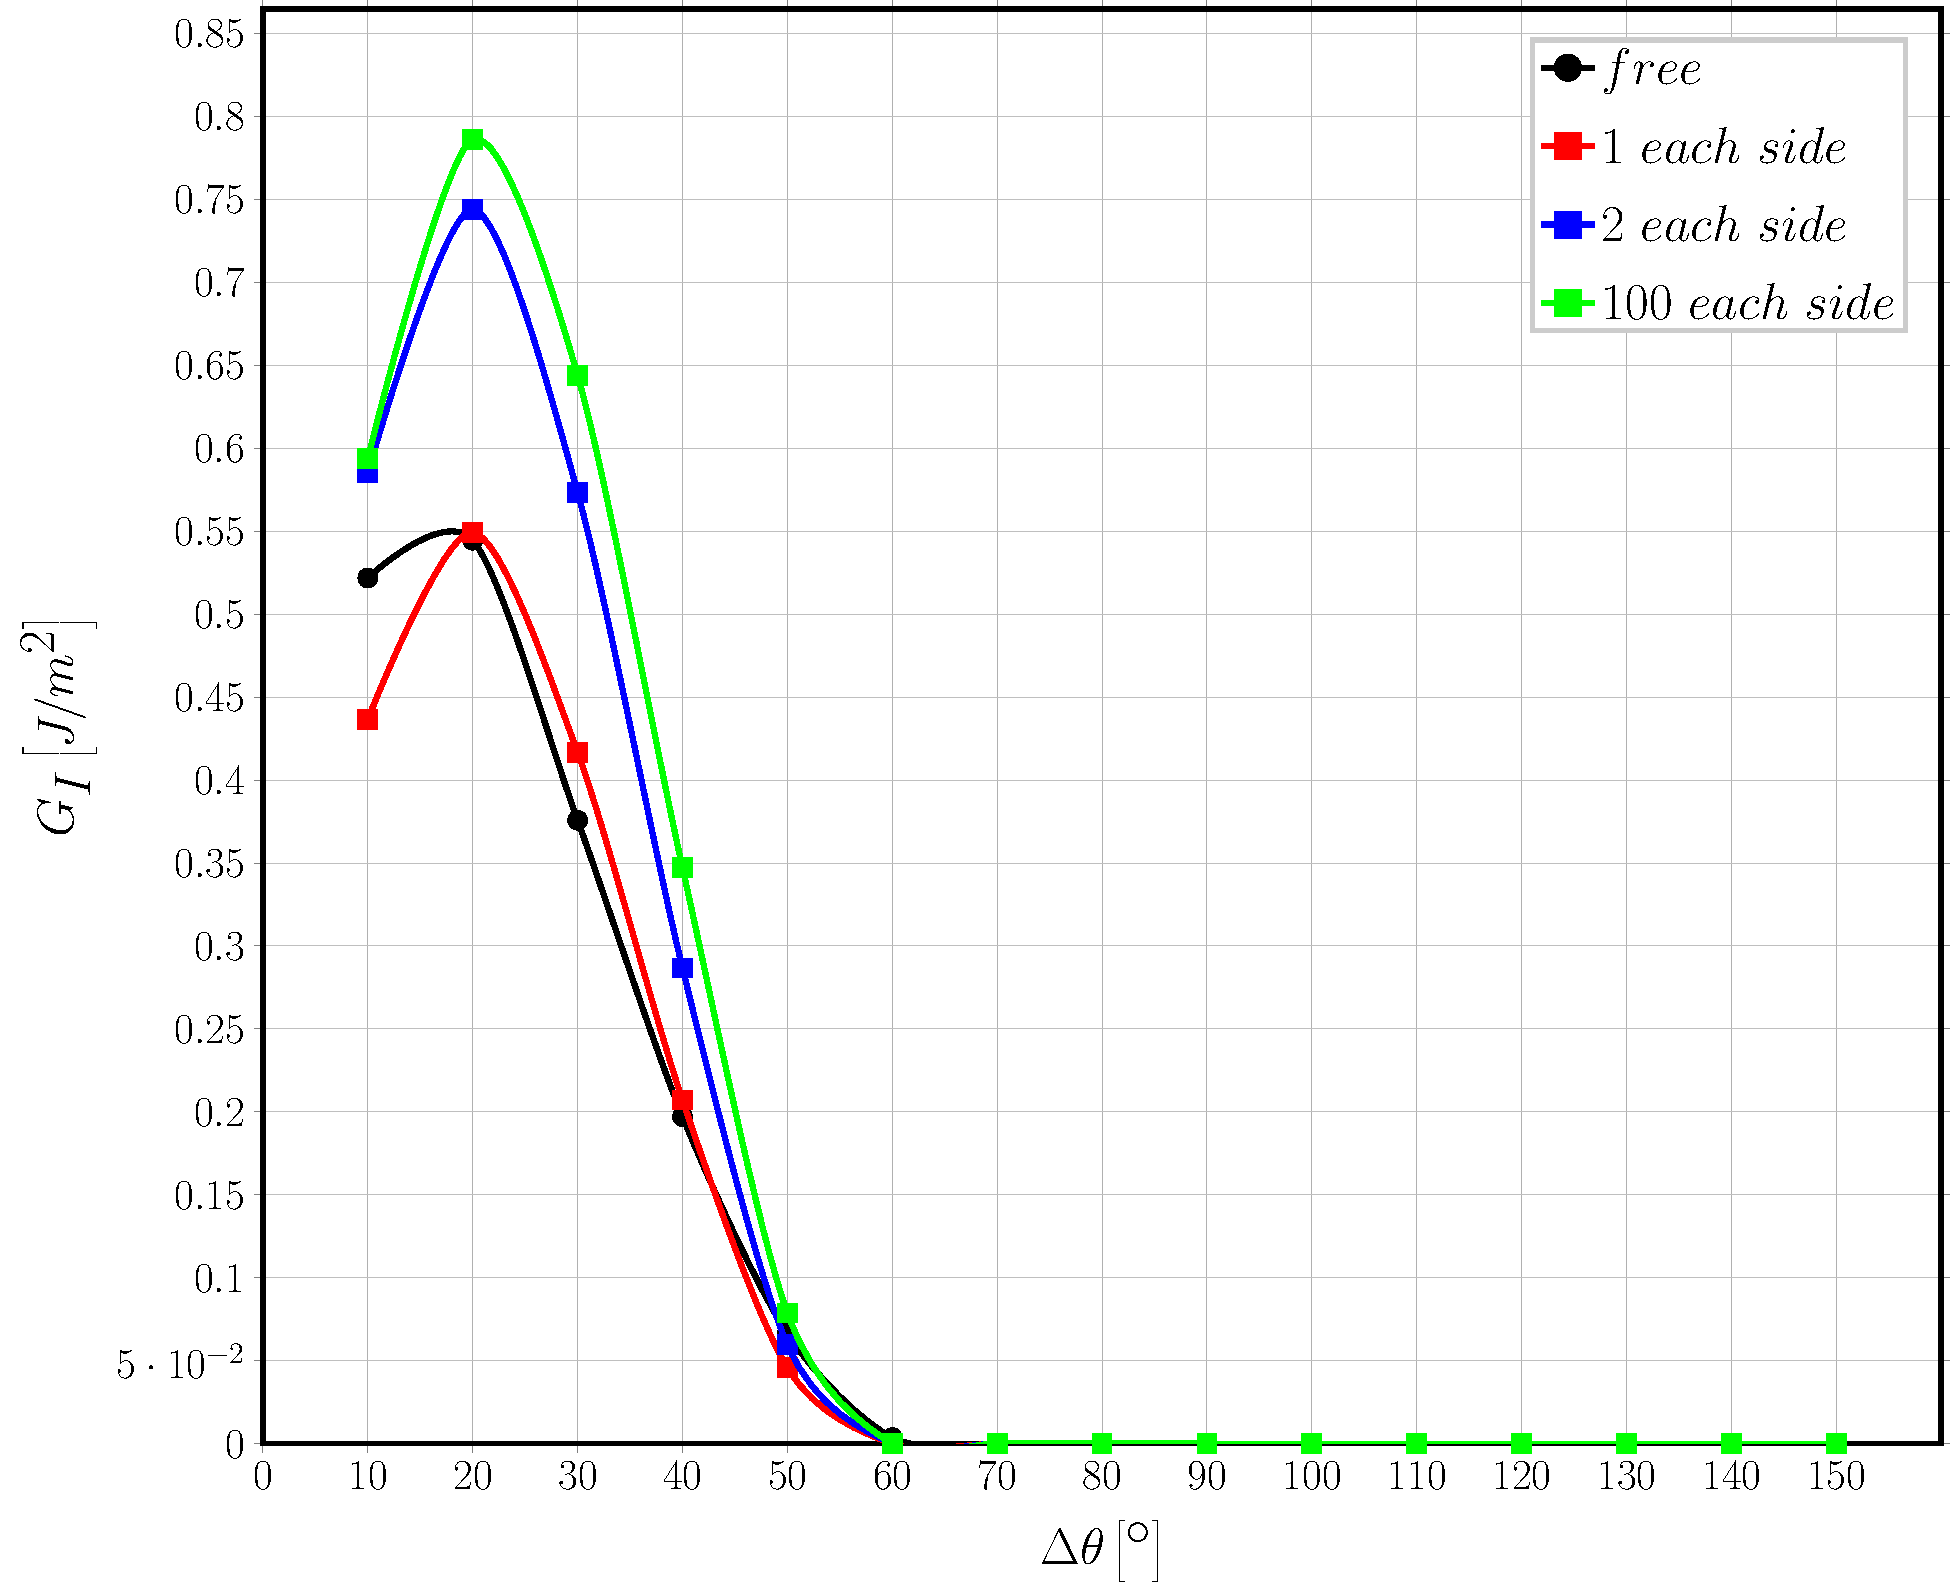
\includegraphics[width=\textwidth]{comparefreesidefibers-vf30-GI.pdf}
        \caption{$V_{f}=30\%$.}\label{subfig:comparisonfree30MI}
    \end{subfigure} ~
    \begin{subfigure}[b]{0.475\textwidth}
        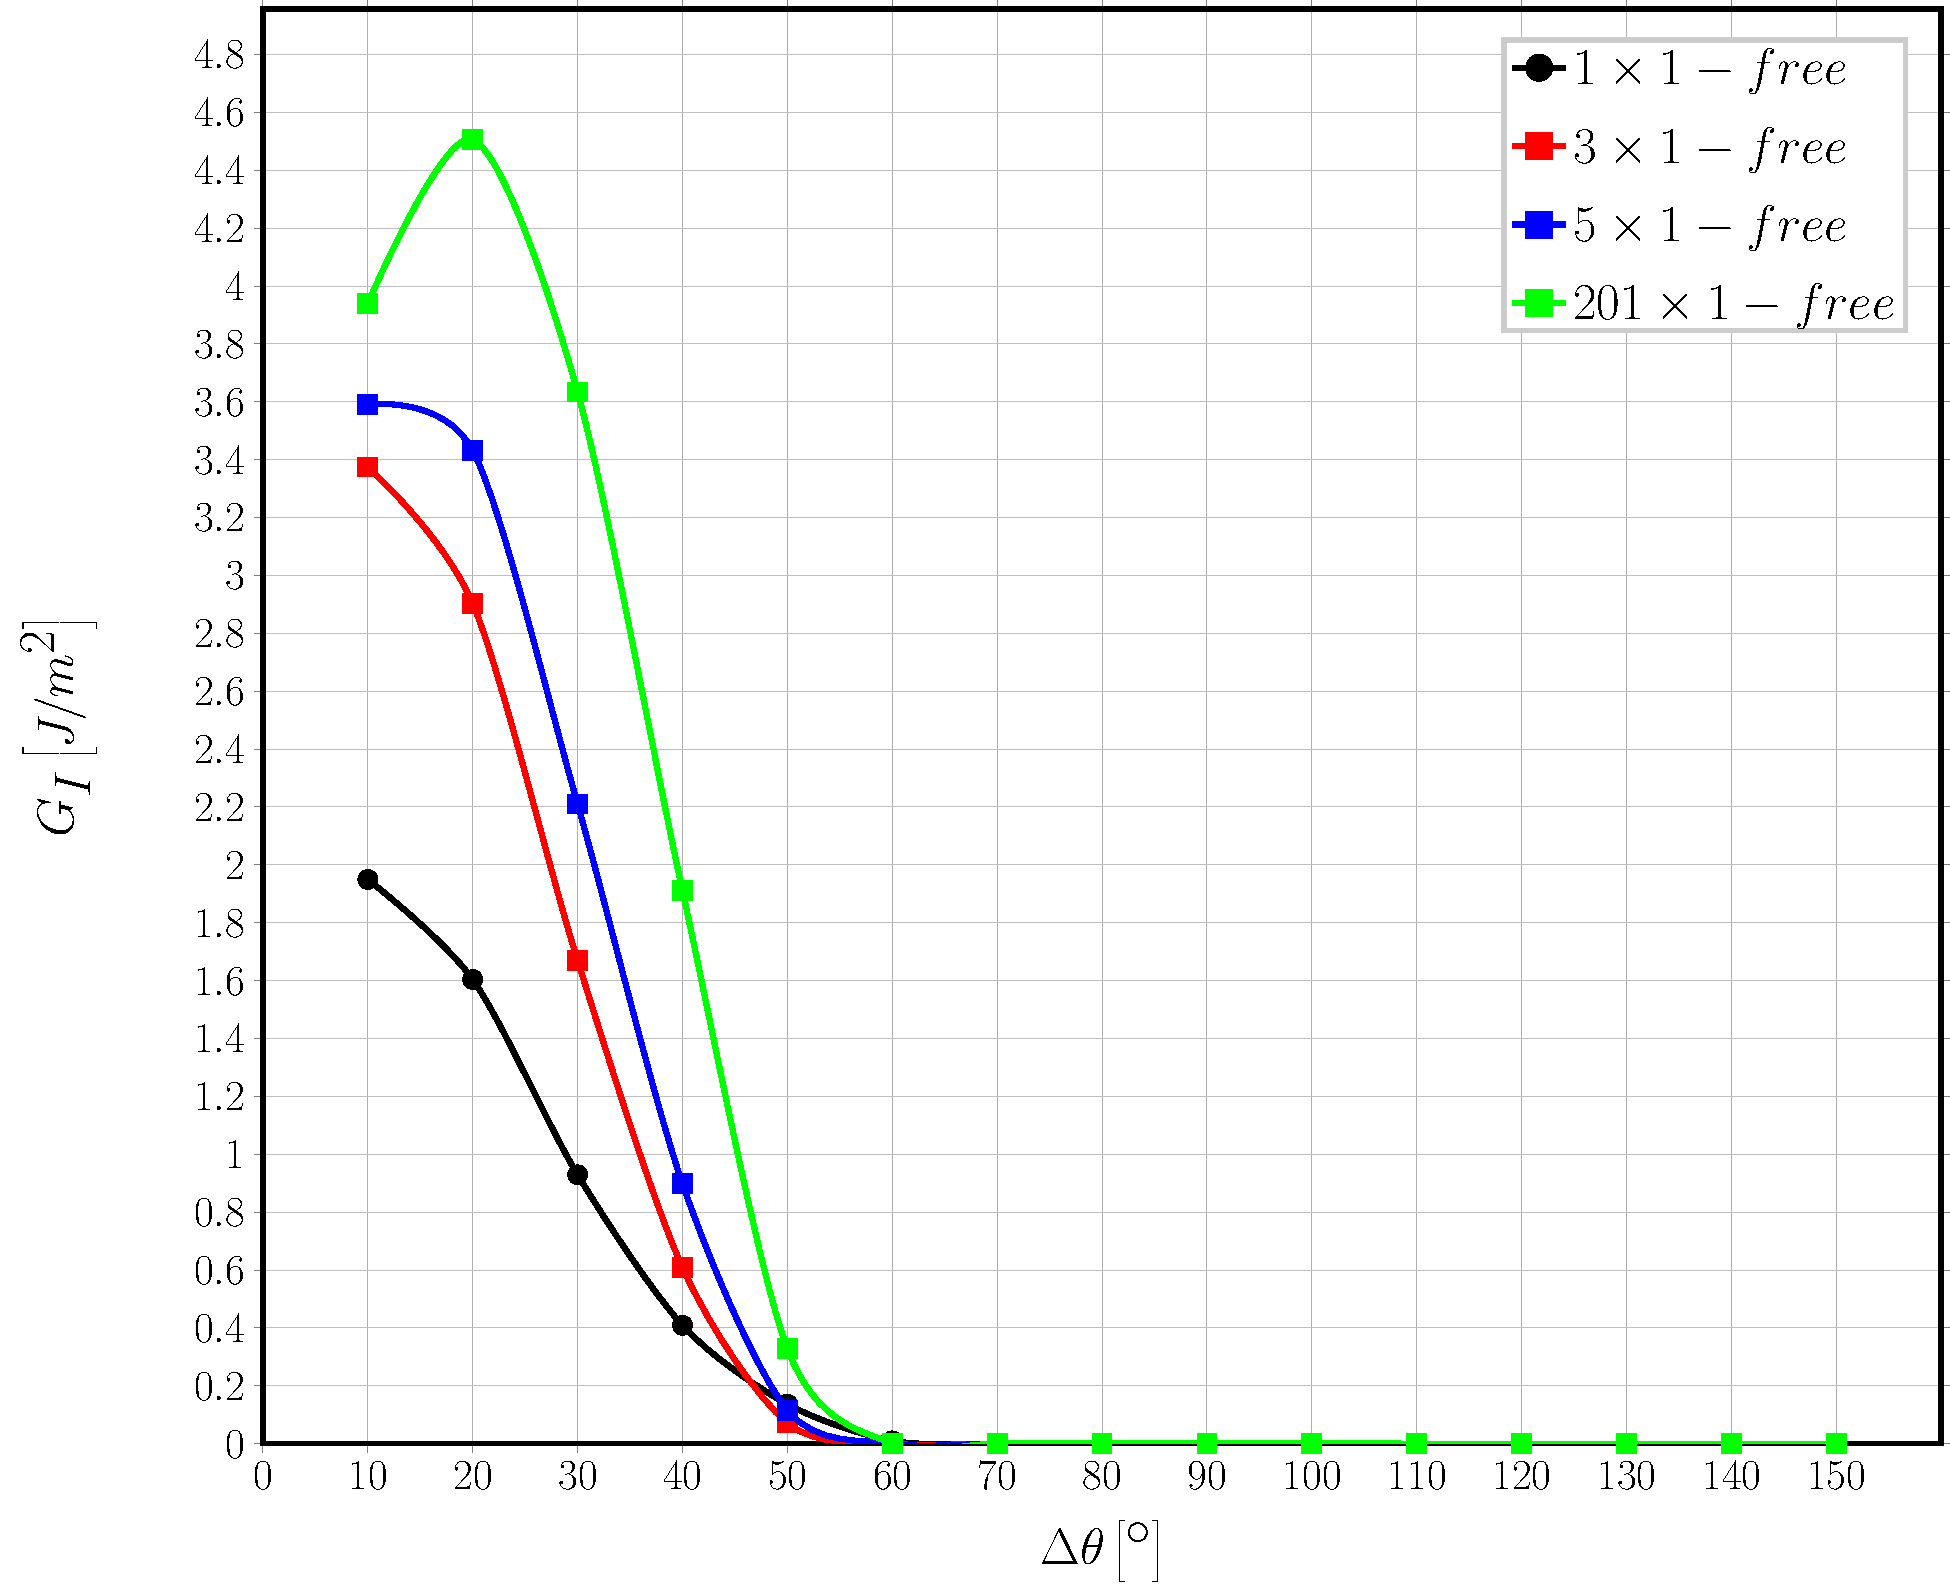
\includegraphics[width=\textwidth]{comparefreesidefibers-vf60-GI.pdf}
        \caption{$V_{f}=60\%$.}\label{subfig:comparisonfree60MI}
    \end{subfigure}

\caption{Comparison of Mode I ERR between the single fiber model with free upper boundary and the multiple fibers model with fibers only on the side at different levels of fiber volume fraction $V_{f}$.}\label{fig:comparisonfreeMI}
\end{figure}

\begin{figure}[!h]
\centering
    \begin{subfigure}[b]{0.475\textwidth}
        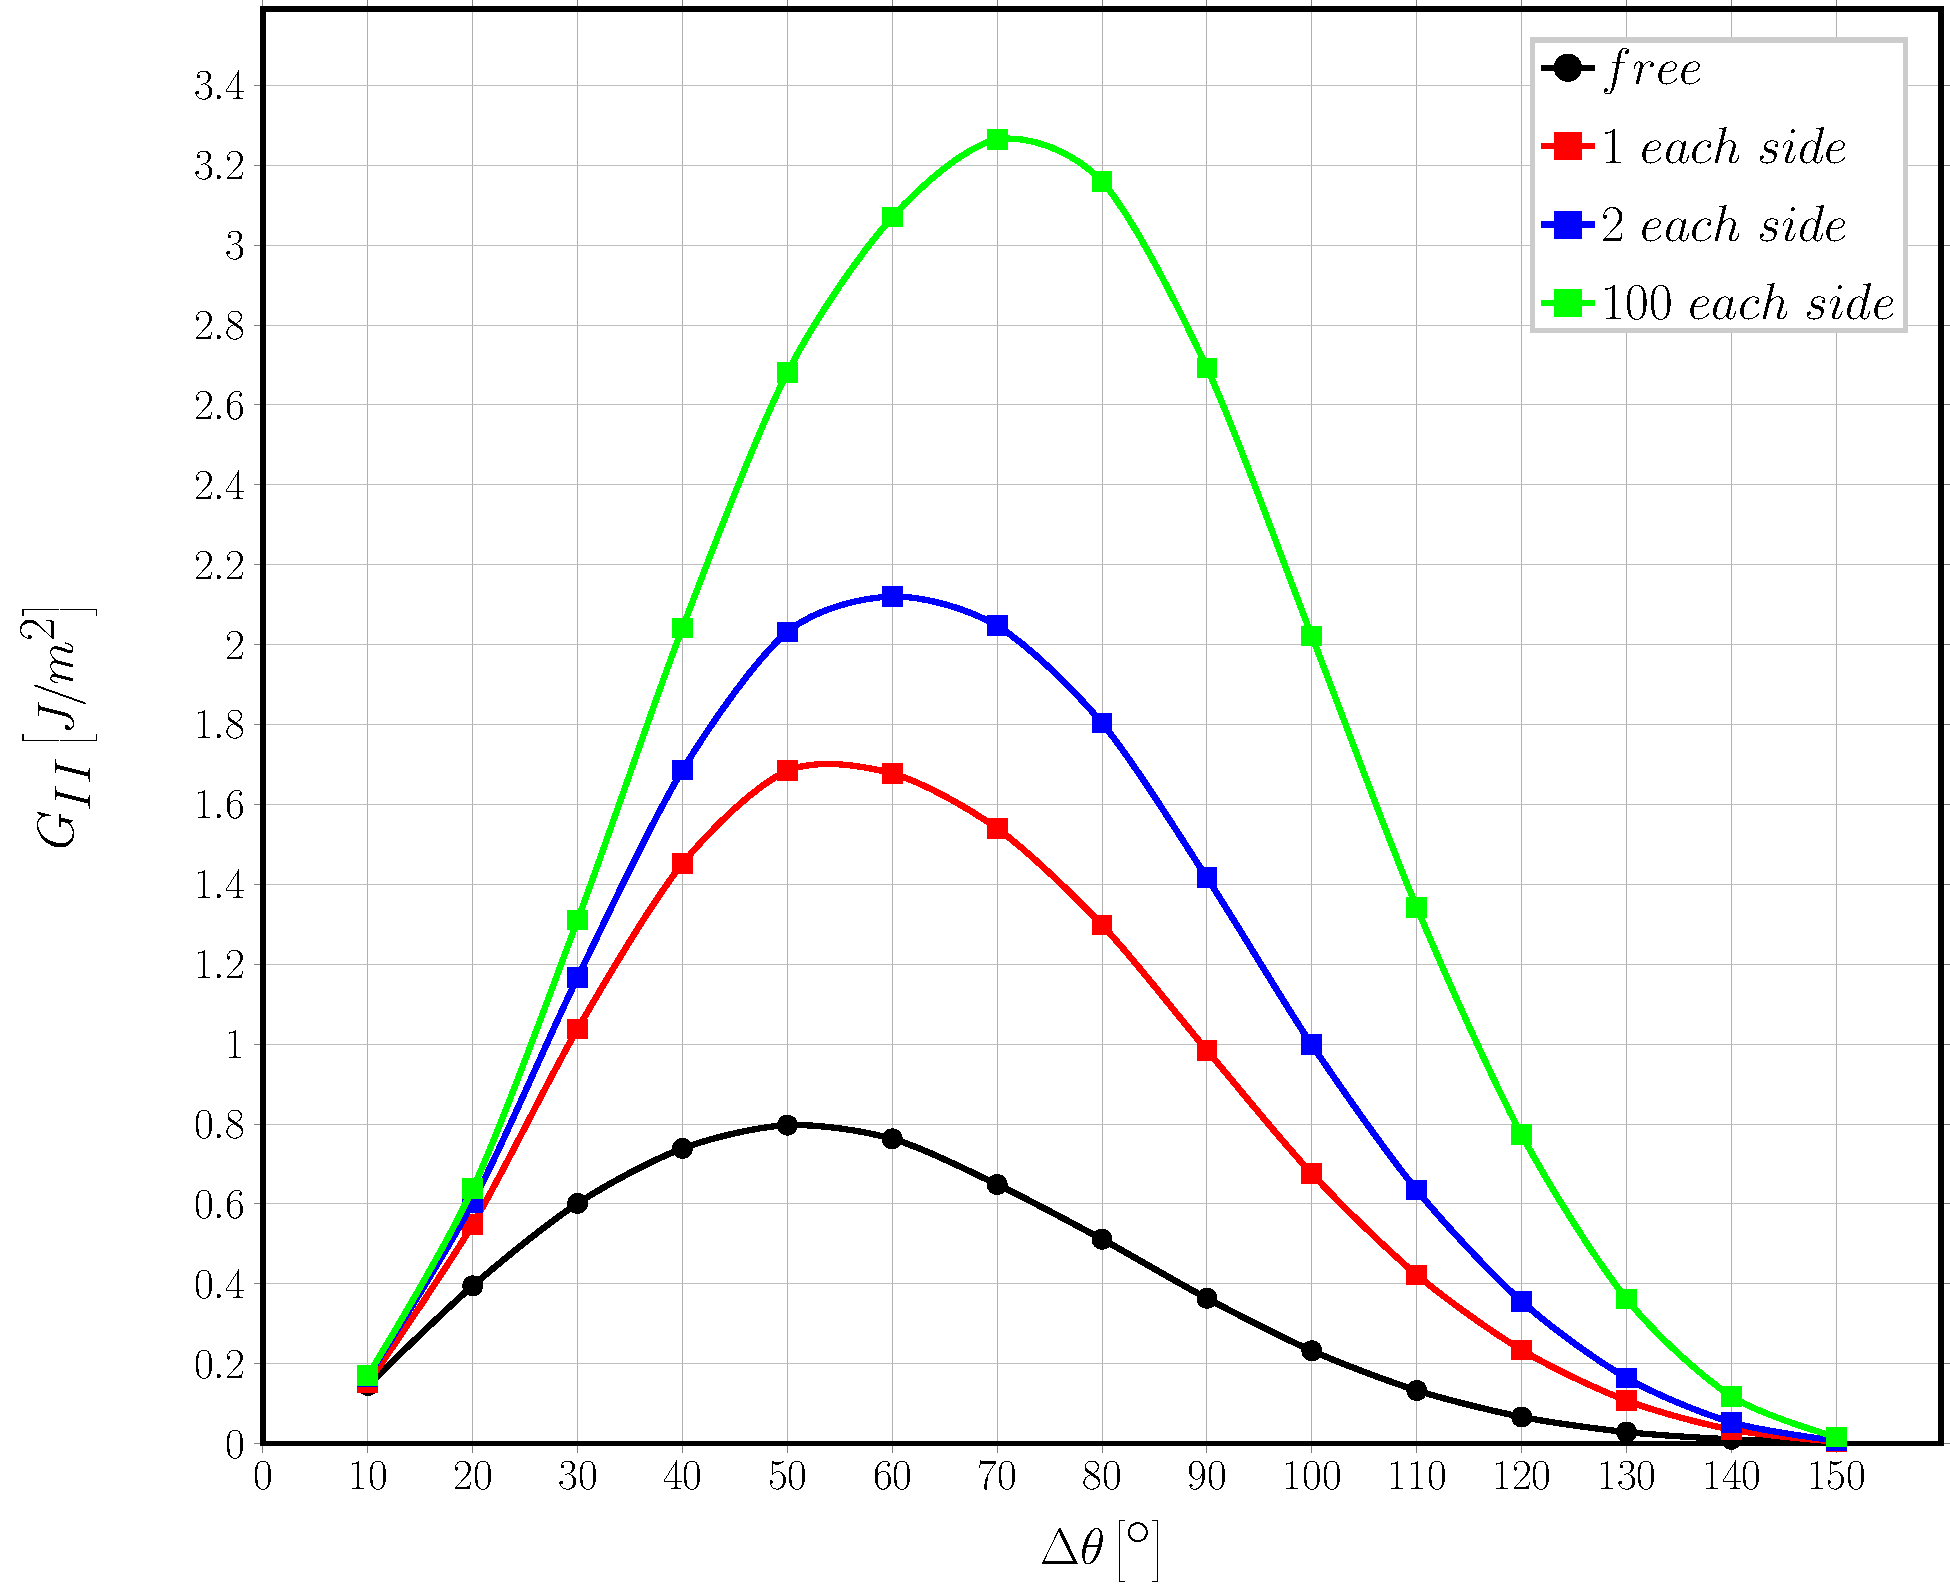
\includegraphics[width=\textwidth]{comparefreesidefibers-vf30-GII.pdf}
        \caption{$V_{f}=30\%$.}\label{subfig:comparisonfree30MII}
    \end{subfigure} ~
    \begin{subfigure}[b]{0.475\textwidth}
        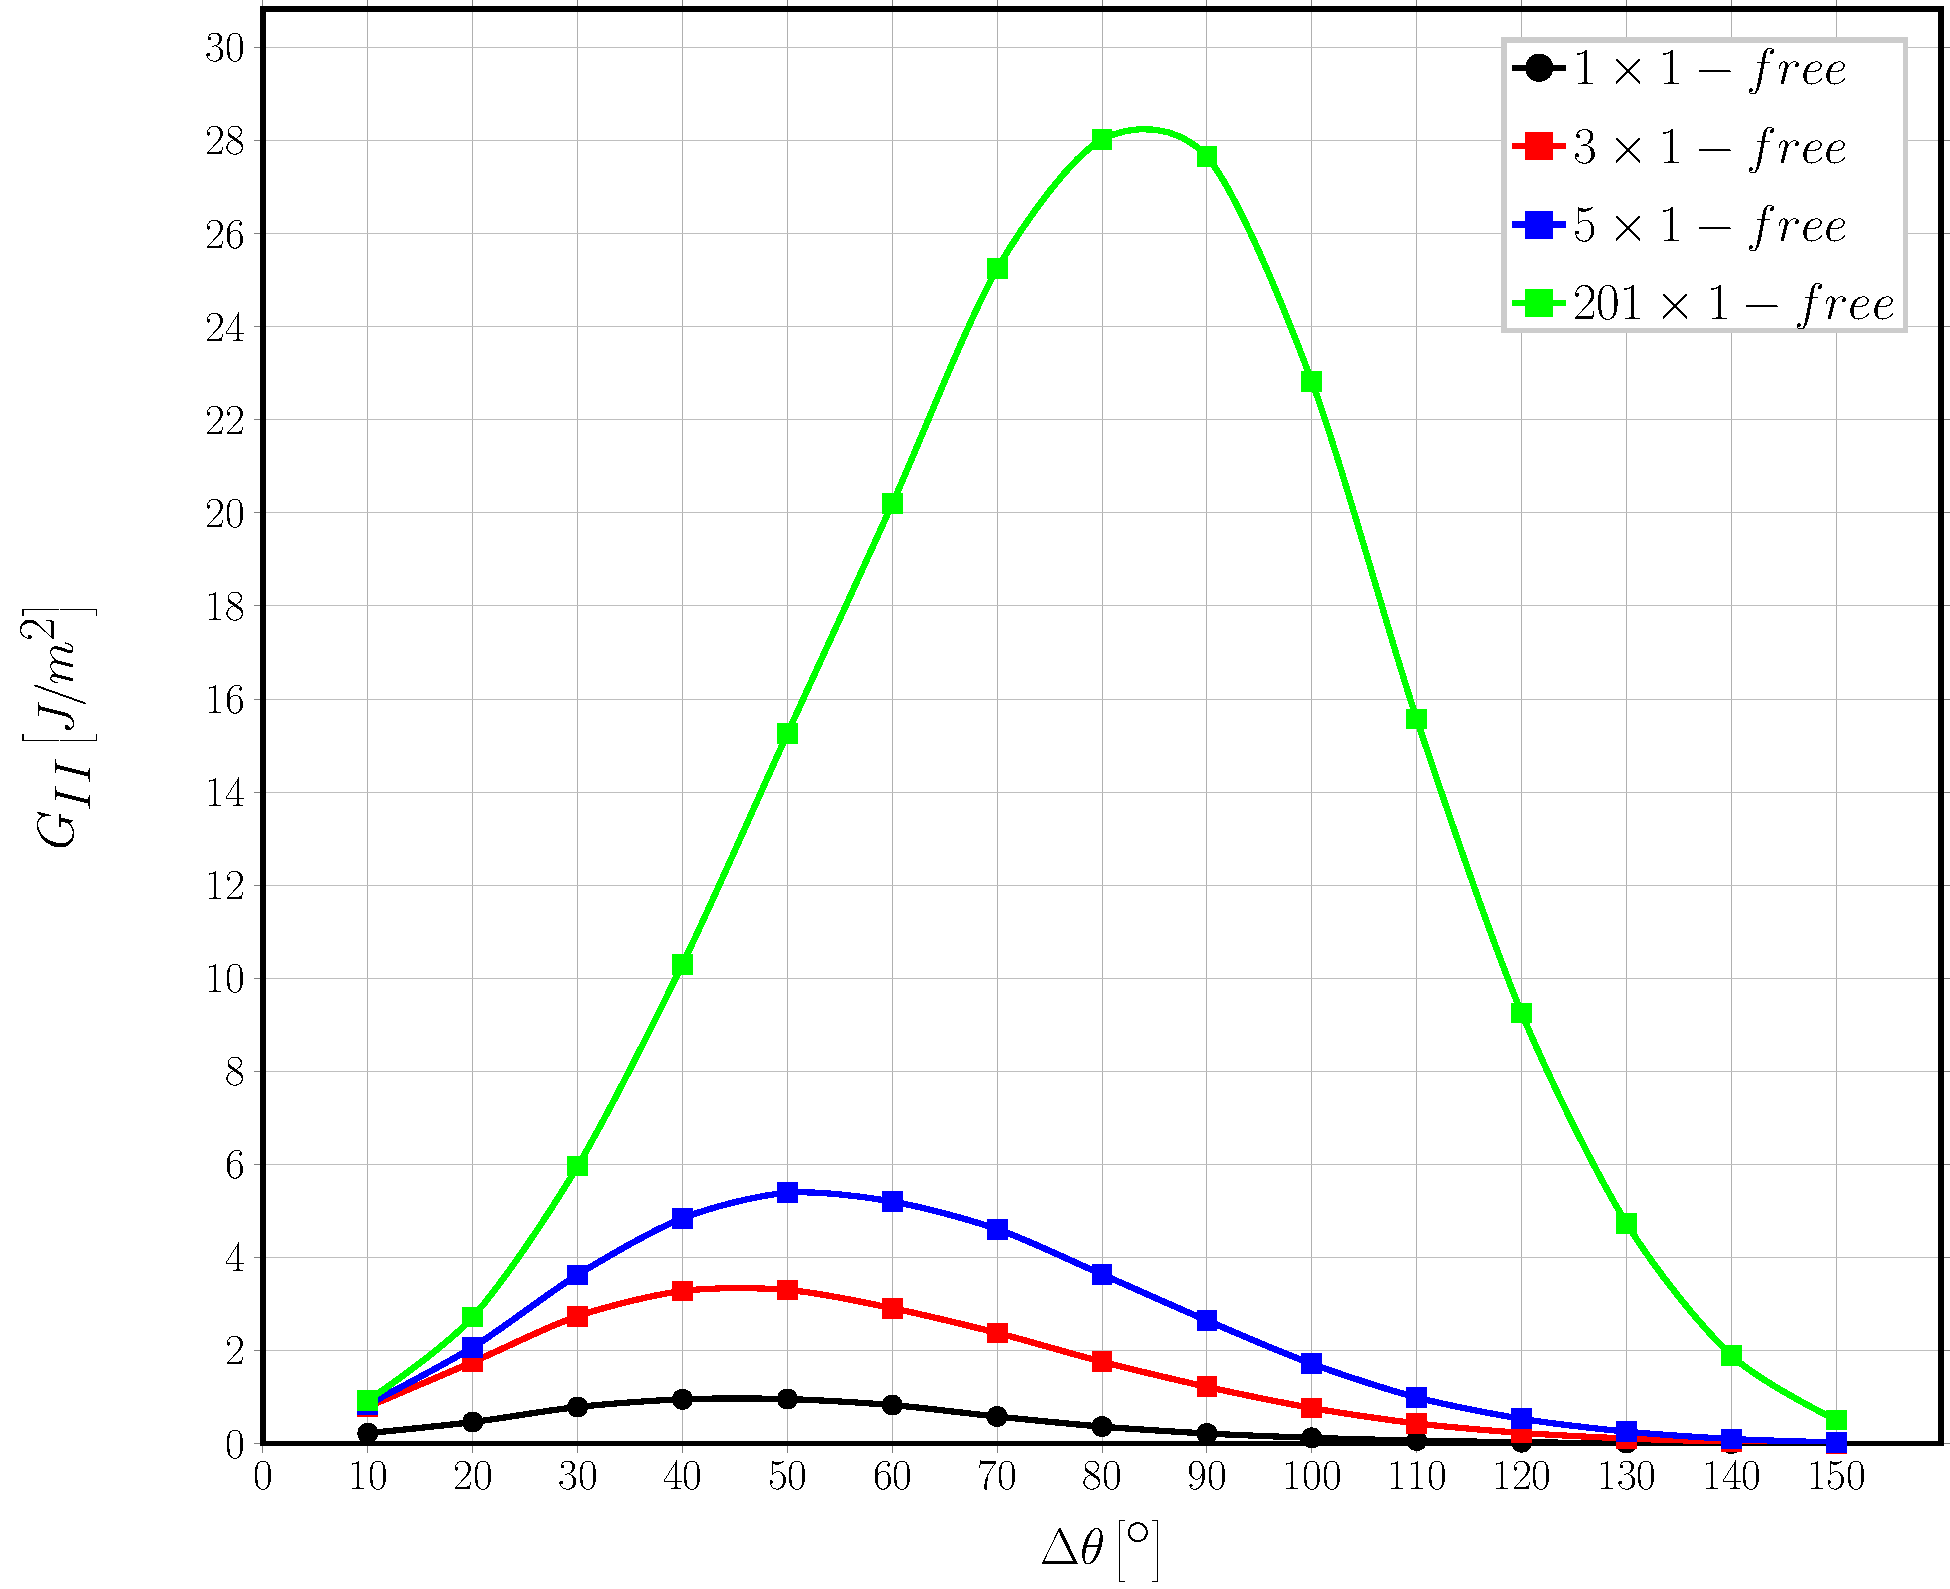
\includegraphics[width=\textwidth]{comparefreesidefibers-vf60-GII.pdf}
        \caption{$V_{f}=60\%$.}\label{subfig:comparisonfree60MII}
    \end{subfigure}

\caption{Comparison of Mode II ERR between the single fiber model with free upper boundary and the multiple fibers model with fibers only on the side at different levels of fiber volume fraction $V_{f}$.}\label{fig:comparisonfreeMII}
\end{figure}

The $1\times 1-coupling$ or coupling model (Figs.~\ref{fig:comparisoncouplingMI} and~\ref{fig:comparisoncouplingMII}) underestimates consistently the ERR in Mode I and Mode II when compared with $n\times k-free$ models, as it represents an infinitely thick UD with all the fibers partially debonded. When compared with the $1\times k-free$ model, it shows interestingly a good agreement, especially in Mode I (Fig.~\ref{subfig:comparisoncoupling30MI}).

\begin{figure}[!h]
\centering
    \begin{subfigure}[b]{0.475\textwidth}
        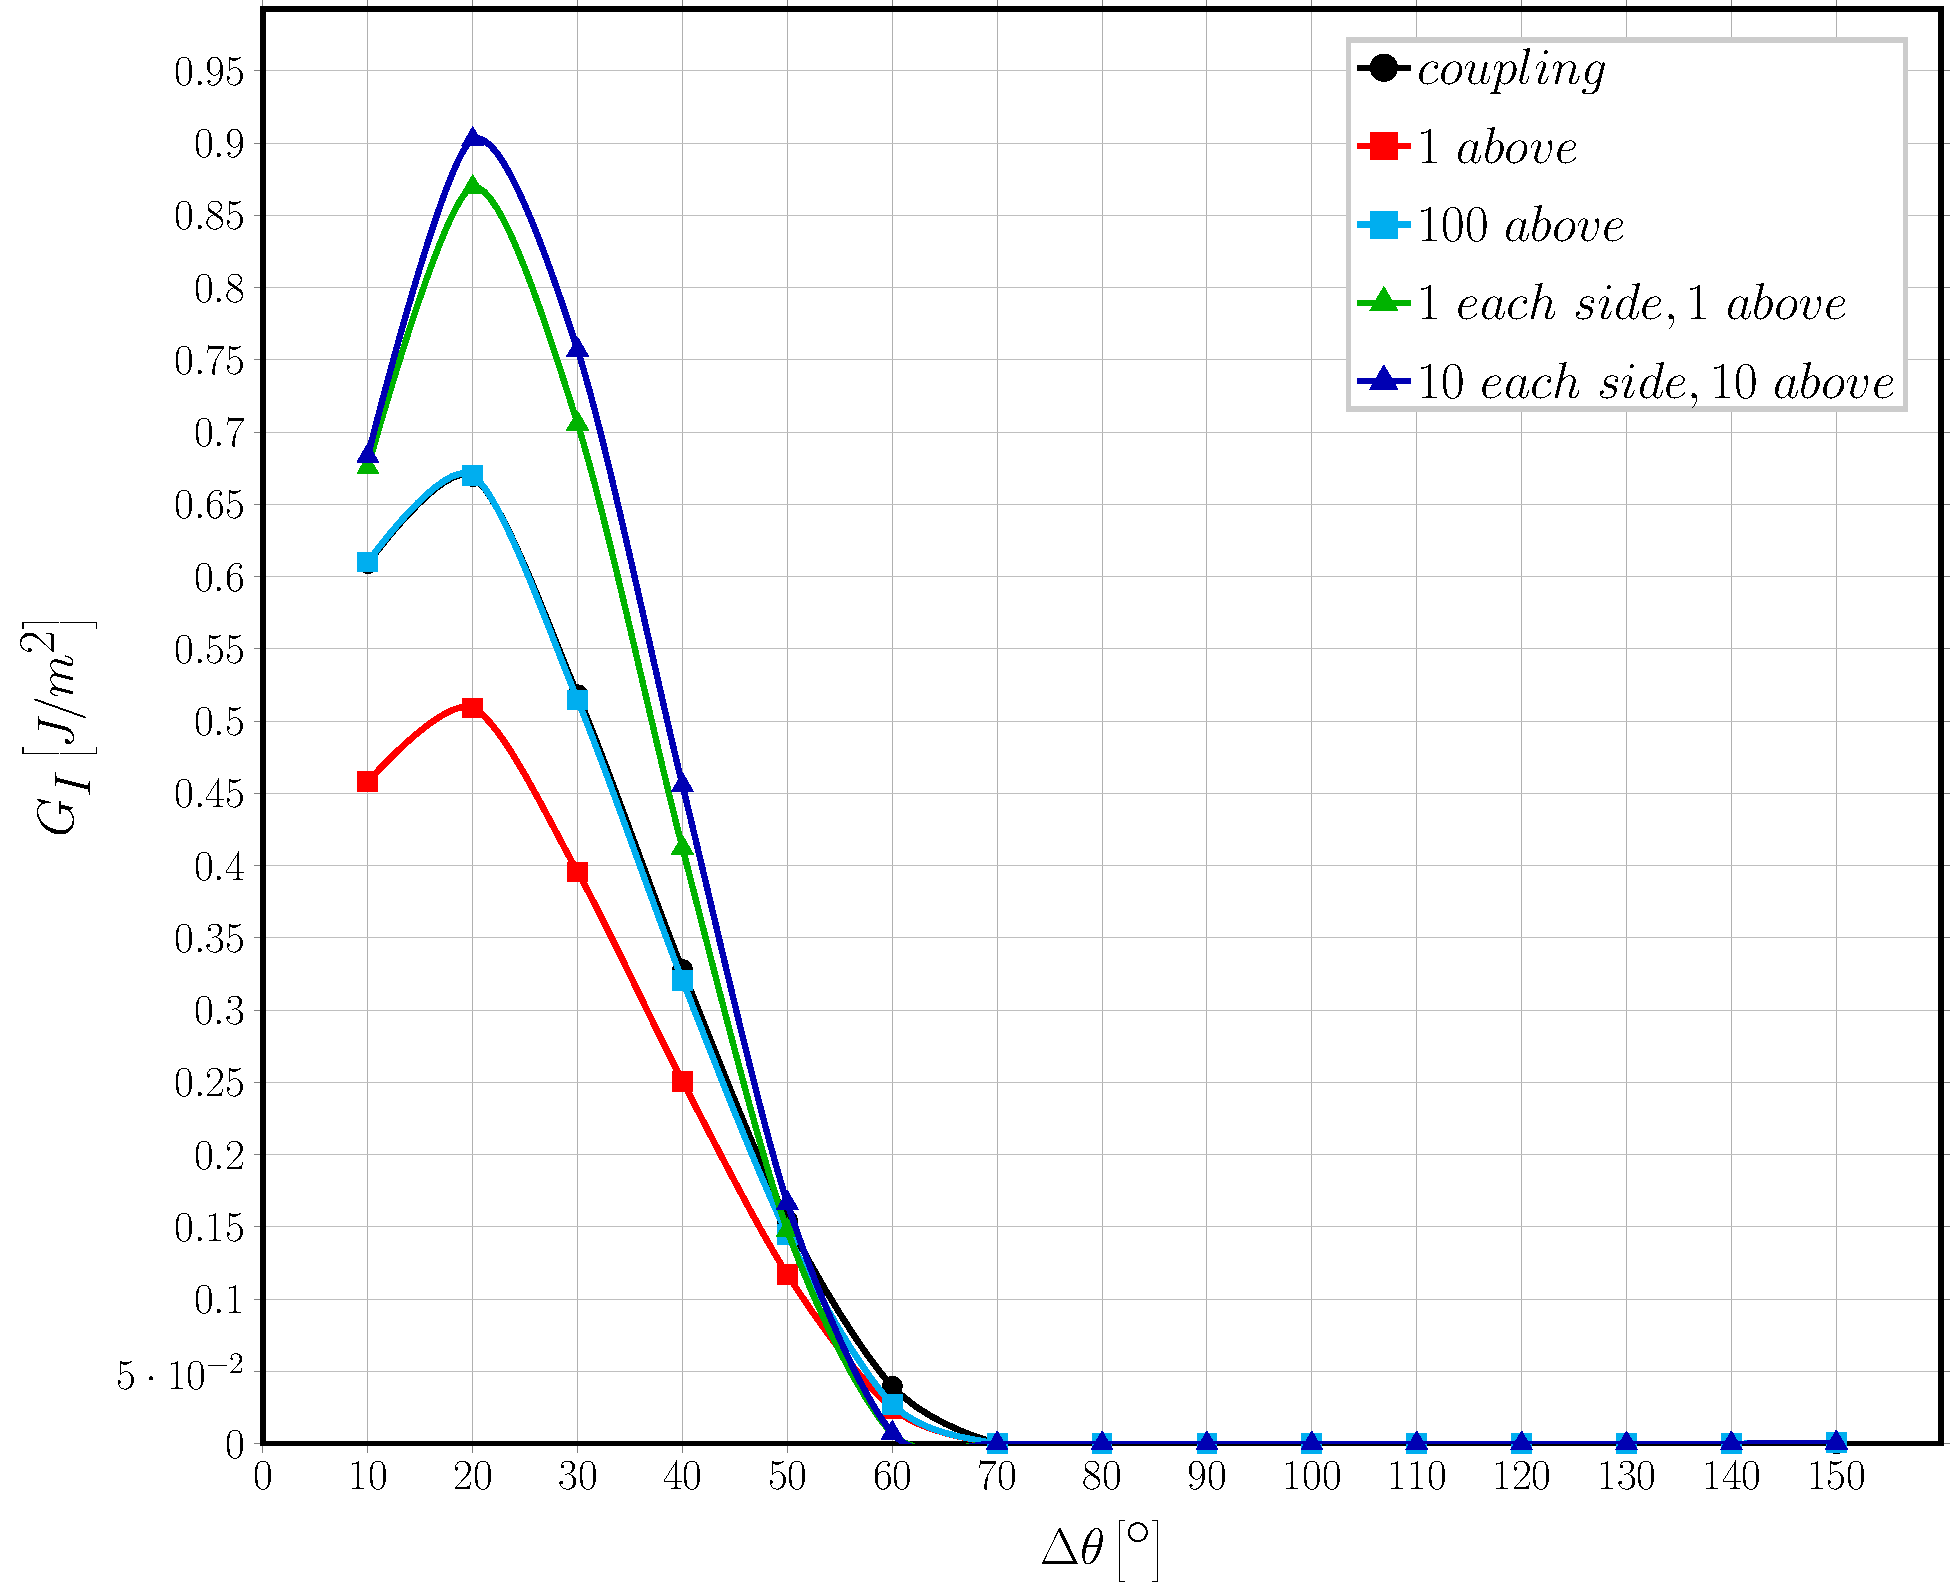
\includegraphics[width=\textwidth]{comparecouplingabovesidefibers-vf30-GI.pdf}
        \caption{$V_{f}=30\%$.}\label{subfig:comparisoncoupling30MI}
    \end{subfigure} ~
    \begin{subfigure}[b]{0.475\textwidth}
        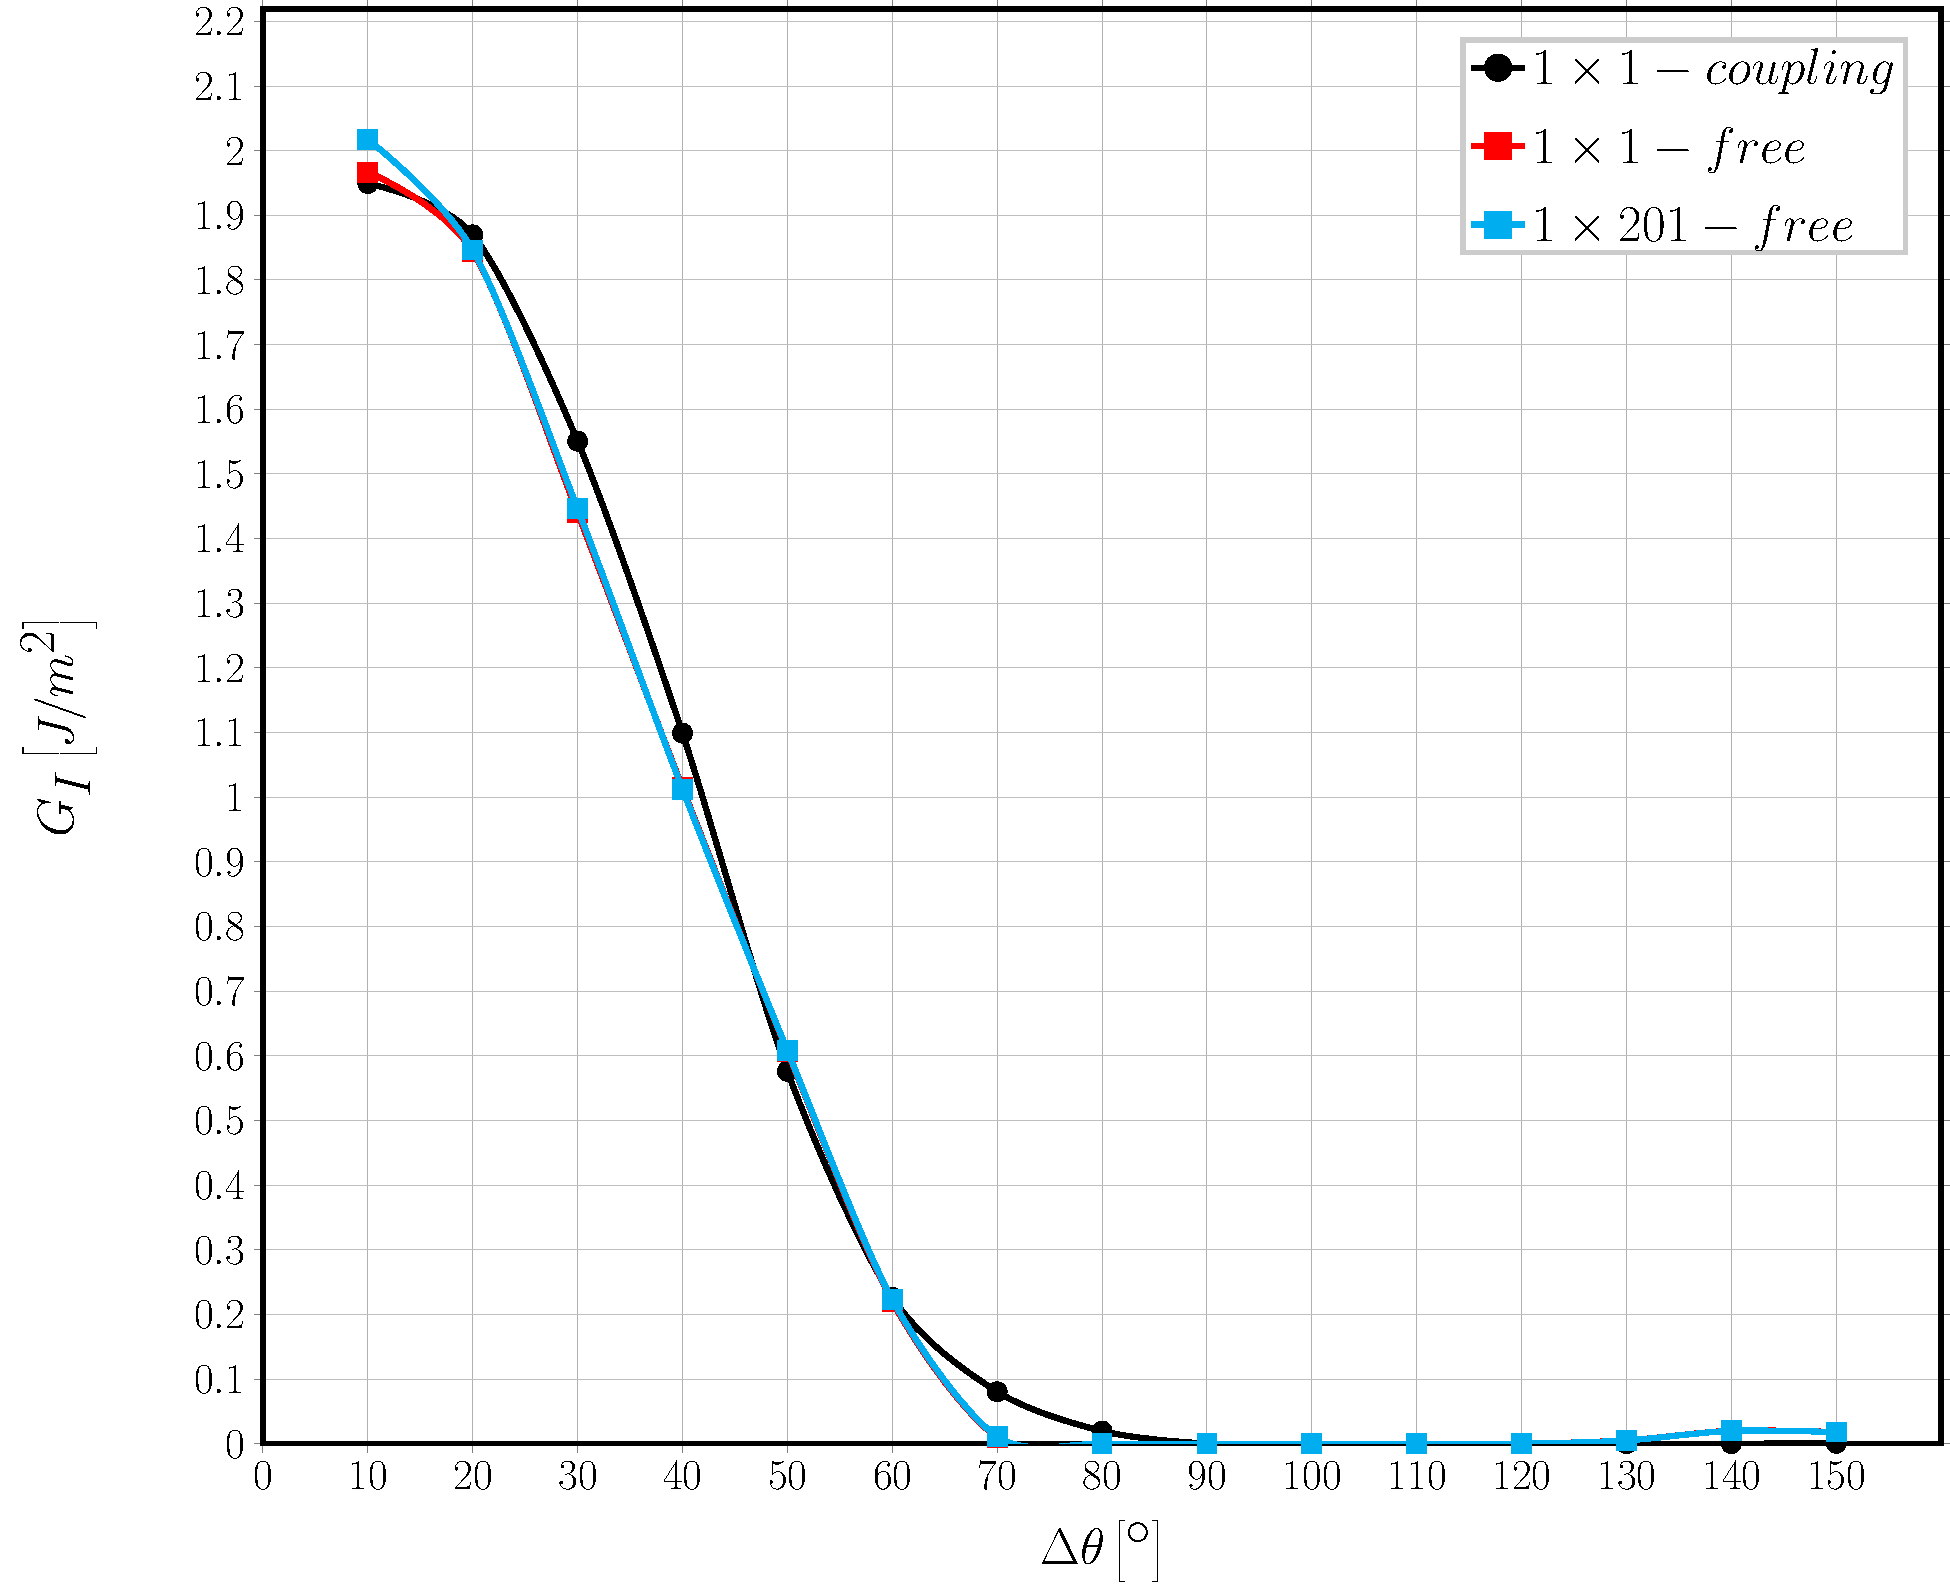
\includegraphics[width=\textwidth]{comparecouplingabovesidefibers-vf60-GI.pdf}
        \caption{$V_{f}=60\%$.}\label{subfig:comparisoncoupling60MI}
    \end{subfigure}

\caption{Comparison of Mode I ERR between the single fiber model with coupling conditions along the upper boundary and the multiple fibers model with fibers above and both above and on the side at different levels of fiber volume fraction $V_{f}$.}\label{fig:comparisoncouplingMI}
\end{figure}

In Mode II, it shows a sizeable difference in the range $50^{\circ}-90^{\circ}$, while its results coincide with those of the $1\times k-free$ model for other values of $\Delta\theta$. These observations point to the evidence that debonds' interaction has a significant effect in the loading direction and not in the transverse one. The lower estimates of $G_{II}$ in the range  $50^{\circ}-90^{\circ}$ are due to the presence of a debond of the same size in the fiber just above the central one (modeled by the coupling boundary condition), which leaves the strip of matrix between the two fibers free to deform away from both fibers due to Poisson's effect and thus favors Mode I and reduces Mode II. This translates in the lower estimates in Fig.~\ref{fig:comparisoncouplingMII} and to the delay in the appearance of the contact zone, particularly evident in Fig.~\ref{subfig:comparisoncoupling60MI}.

\begin{figure}[!h]
\centering
    \begin{subfigure}[b]{0.475\textwidth}
        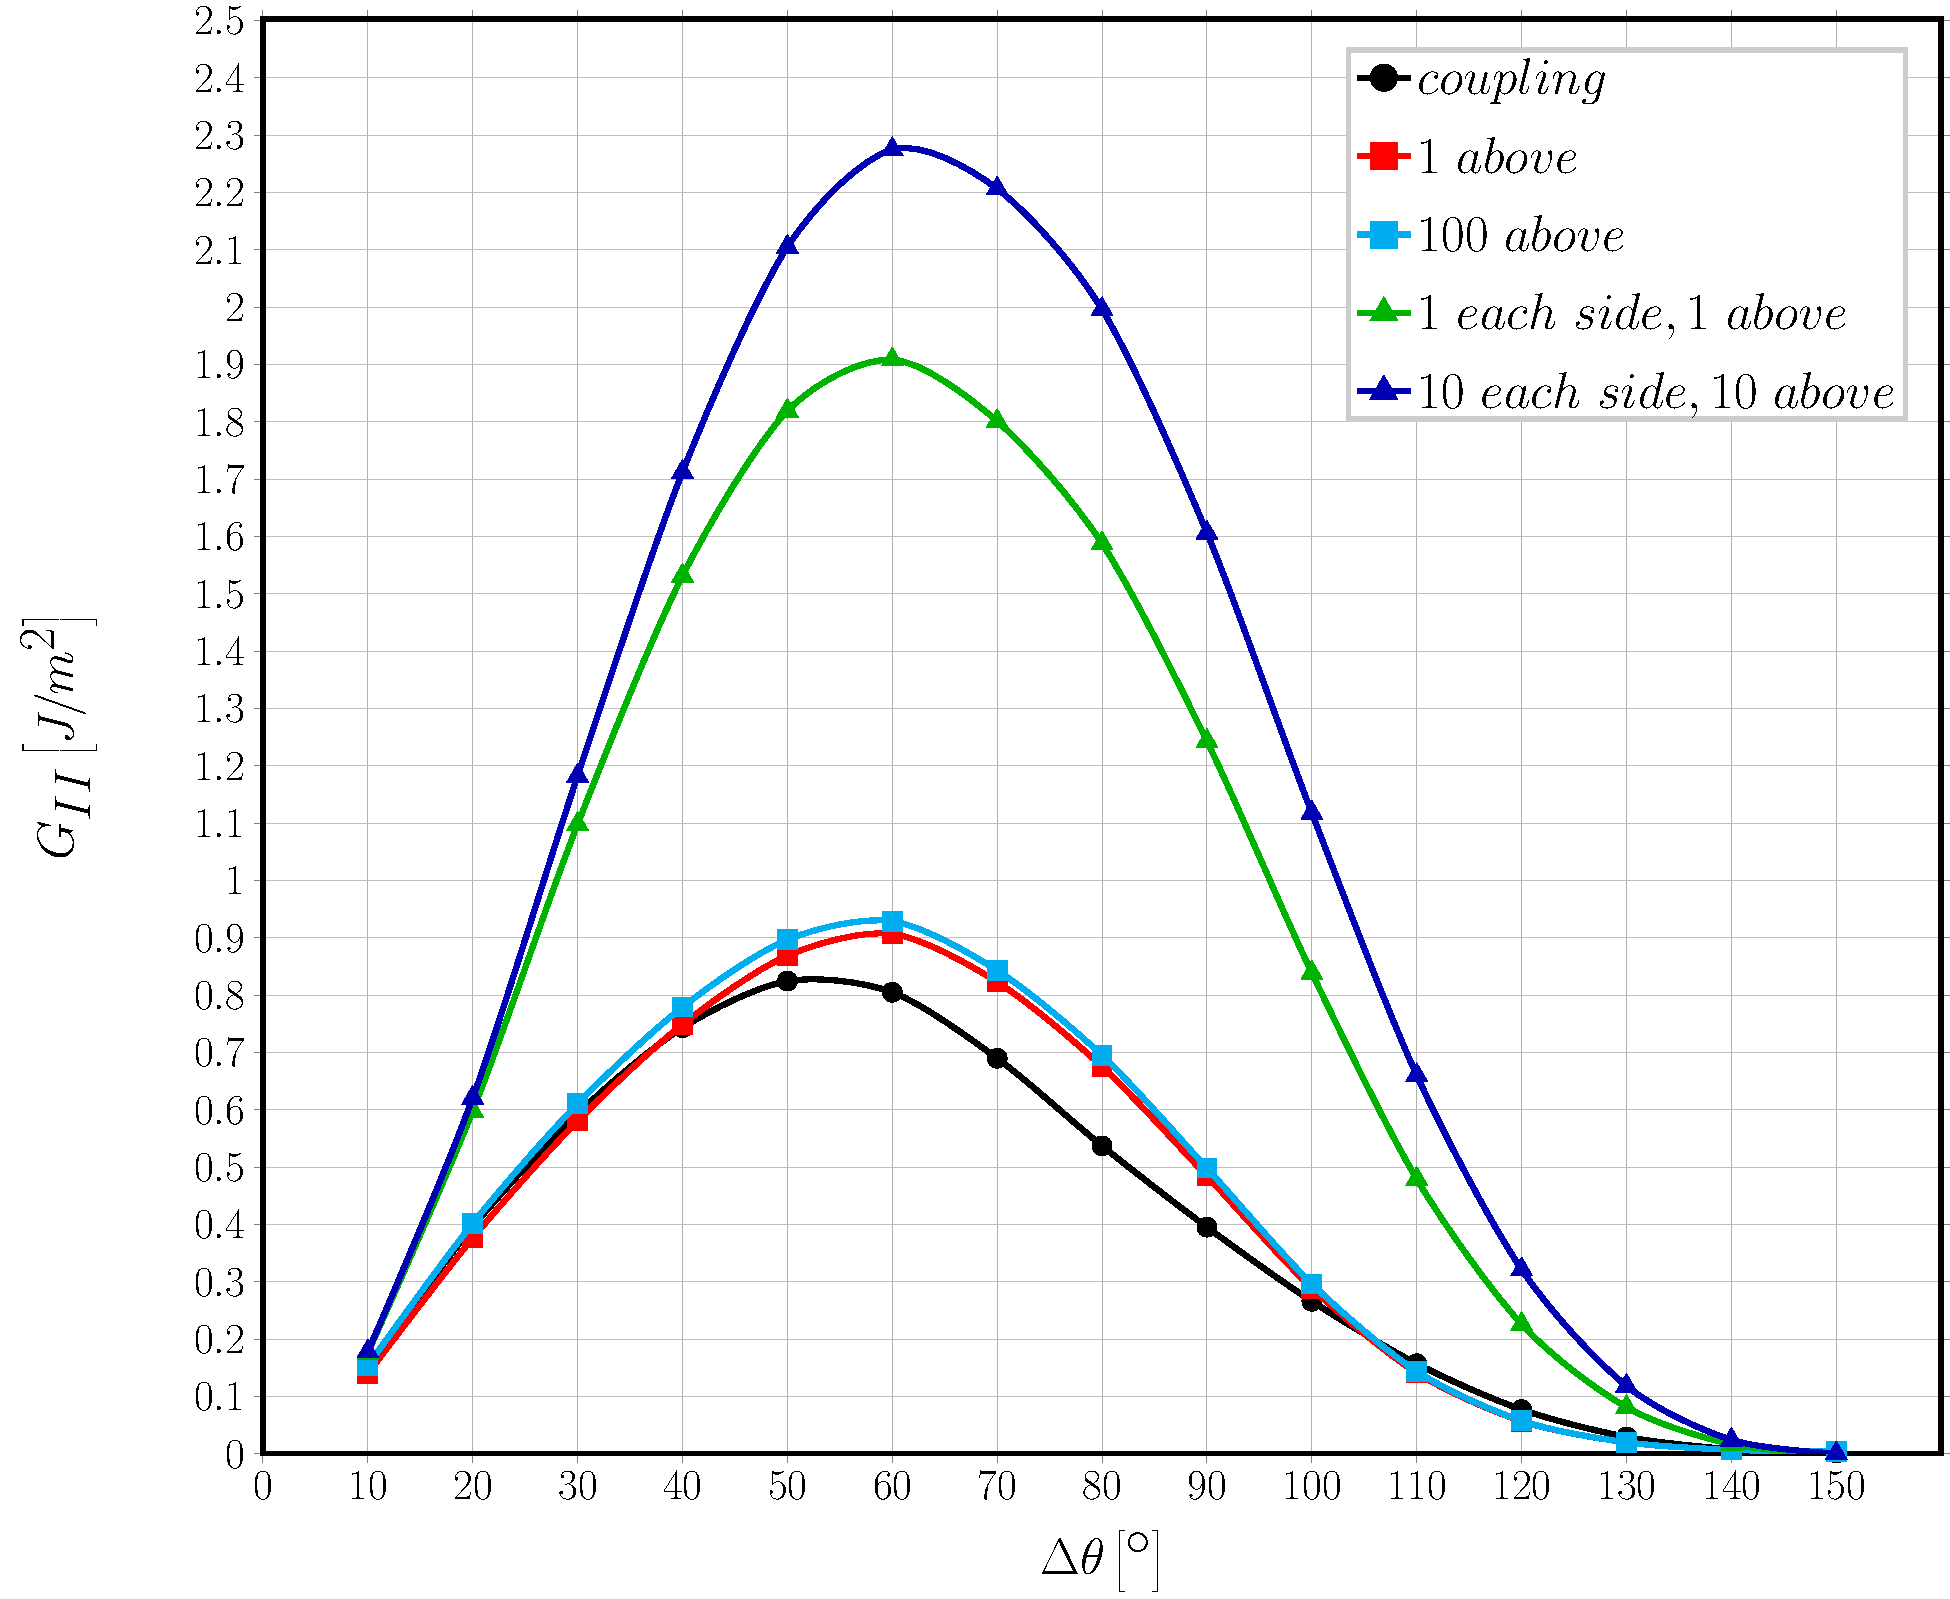
\includegraphics[width=\textwidth]{comparecouplingabovesidefibers-vf30-GII.pdf}
        \caption{$V_{f}=30\%$.}\label{subfig:comparisoncoupling30MII}
    \end{subfigure} ~
    \begin{subfigure}[b]{0.475\textwidth}
        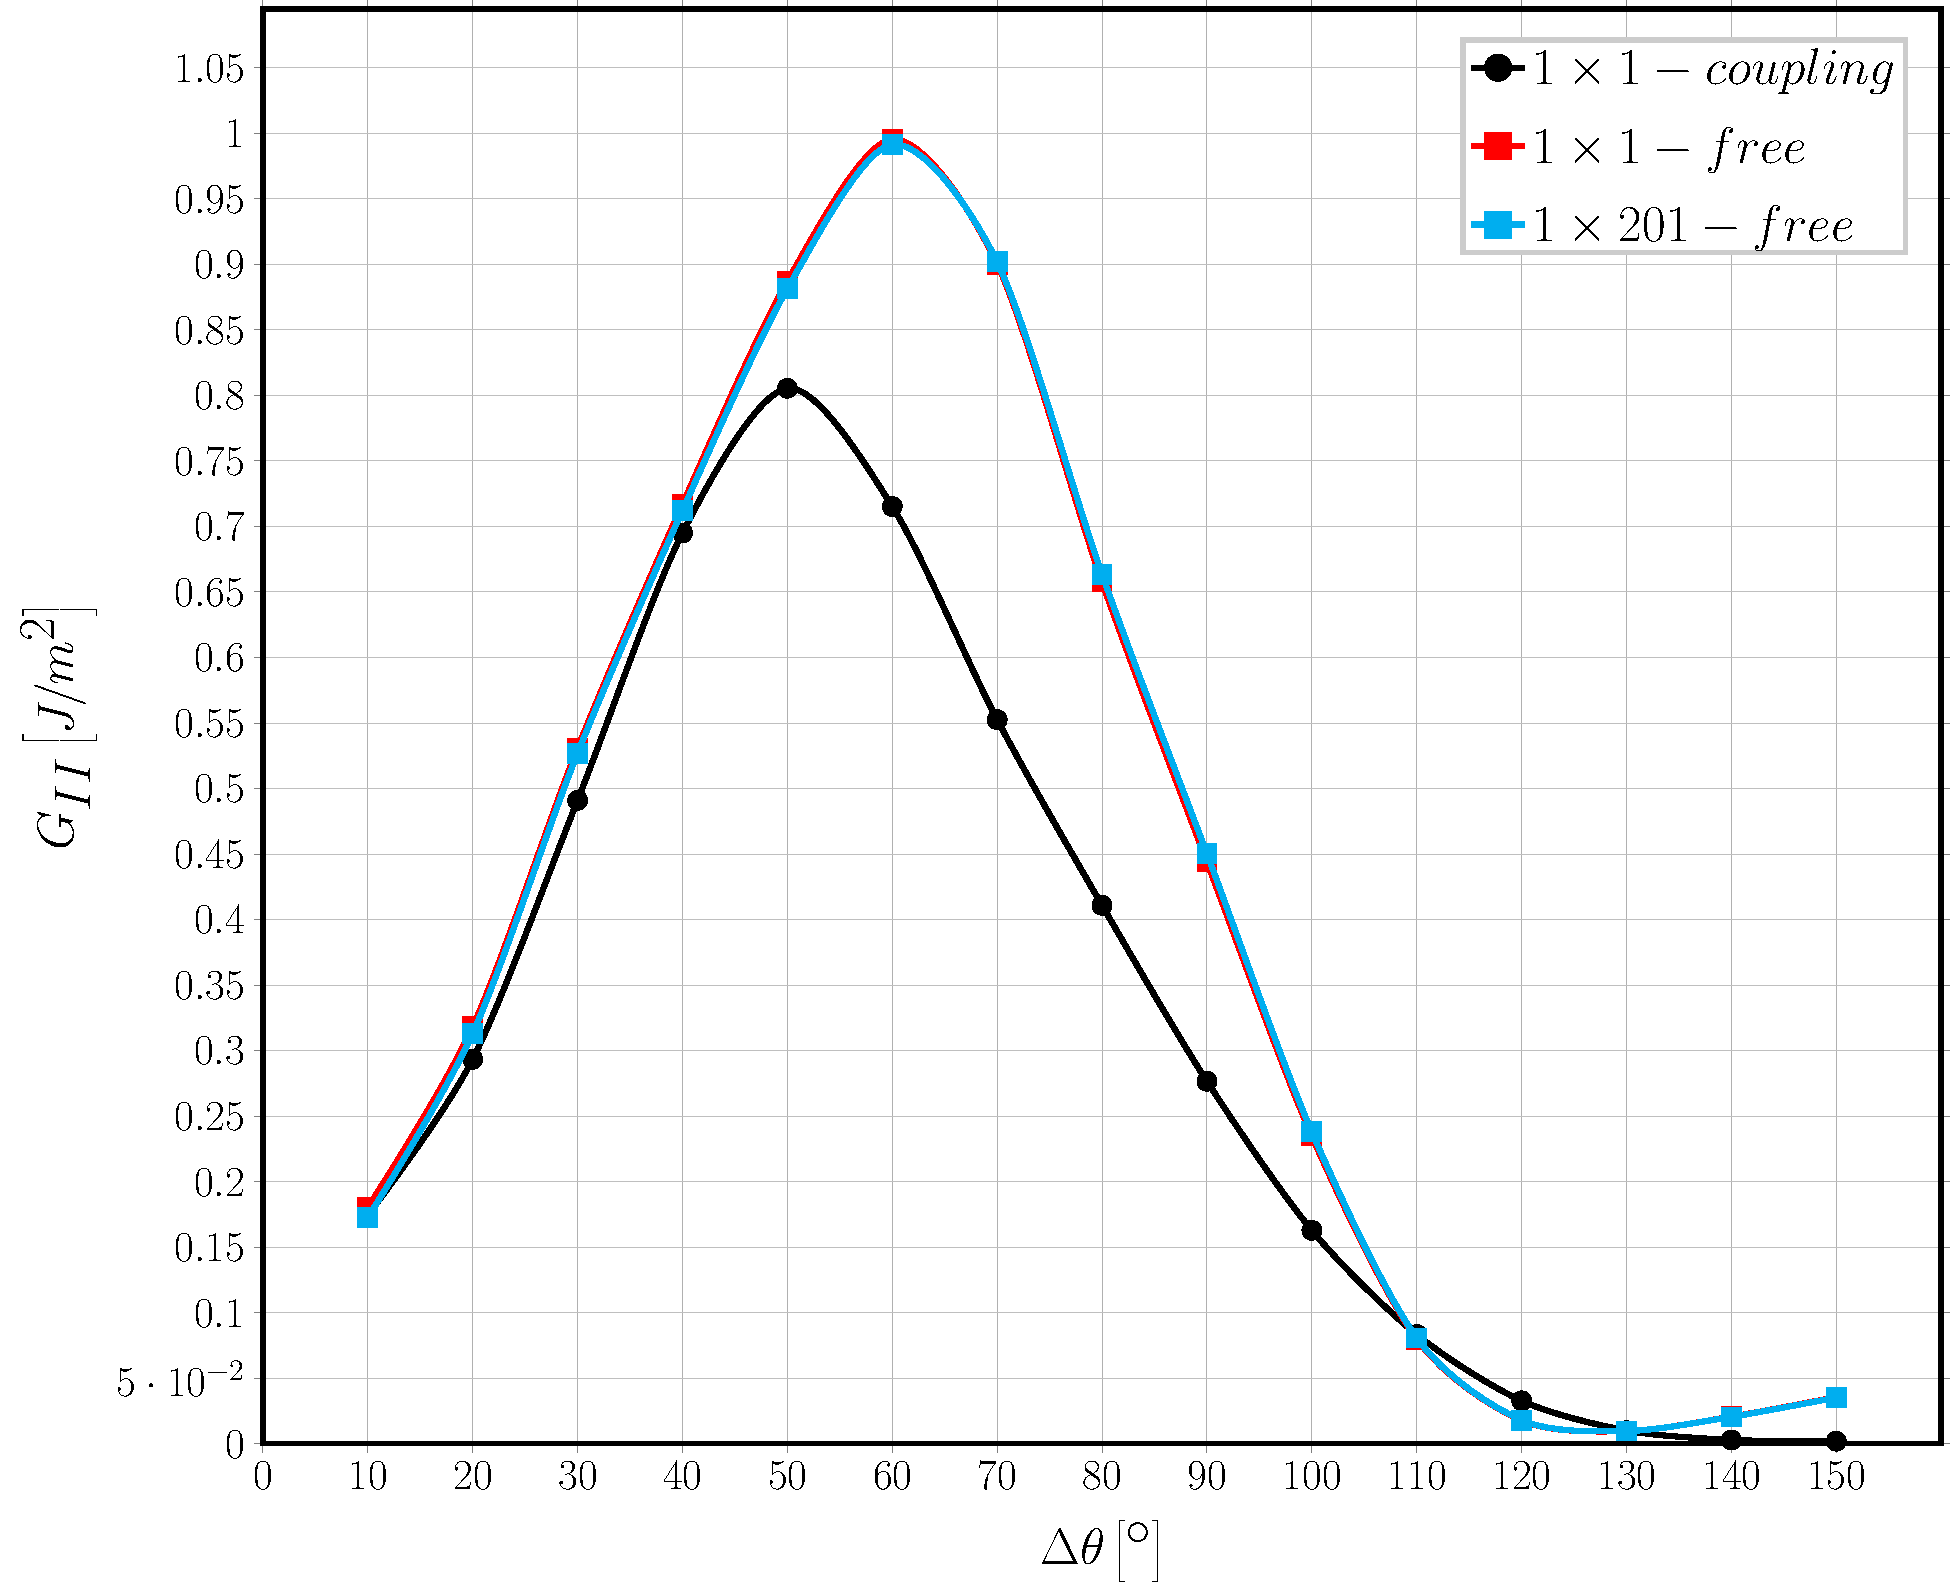
\includegraphics[width=\textwidth]{comparecouplingabovesidefibers-vf60-GII.pdf}
        \caption{$V_{f}=60\%$.}\label{subfig:comparisoncoupling60MII}
    \end{subfigure}

\caption{Comparison of Mode II ERR between the single fiber model with coupling conditions along the upper boundary and the multiple fibers model with fibers above and both above and on the side at different levels of fiber volume fraction $V_{f}$.}\label{fig:comparisoncouplingMII}
\end{figure}

\section{Conclusions \& Outlook}

\section*{Acknowledgements}

Luca Di Stasio gratefully acknowledges the support of the European School of Materials (EUSMAT) through the DocMASE Doctoral Programme and the European Commission through the Erasmus Mundus Programme.

\bibliography{refs}

\end{document}
